% options:
% thesis=B bachelor's thesis
% thesis=M master's thesis
% czech thesis in Czech language
% slovak thesis in Slovak language
% english thesis in English language
% hidelinks remove colour boxes around hyperlinks

\documentclass[thesis=M,czech]{FITthesis}[2012/06/26]

\usepackage[utf8]{inputenc} % LaTeX source encoded as UTF-8

\usepackage{float}

\usepackage{listings}
\usepackage{algorithm}
\usepackage{algorithmic}
\usepackage{listings}
\usepackage{algorithm}
\usepackage{algorithmic}

\usepackage{graphicx} %graphics files inclusion
% \usepackage{amsmath} %advanced maths
% \usepackage{amssymb} %additional math symbols

\usepackage{dirtree} %directory tree visualisation
\usepackage{listings}

\lstdefinelanguage{VHDL}{
	morekeywords={
		CALL,FUNCTION,DESTINATION,EXPORTING,IMPORTING
	}
}

\lstdefinelanguage{java}{
	morekeywords={
	function, return, if, this, that, var, public, class, void, throws, Exception, static
	}
}


% % list of acronyms
% \usepackage[acronym,nonumberlist,toc,numberedsection=autolabel]{glossaries}
% \iflanguage{czech}{\renewcommand*{\acronymname}{Seznam pou{\v z}it{\' y}ch zkratek}}{}
% \makeglossaries

\newcommand{\tg}{\mathop{\mathrm{tg}}} %cesky tangens
\newcommand{\cotg}{\mathop{\mathrm{cotg}}} %cesky cotangens

% % % % % % % % % % % % % % % % % % % % % % % % % % % % % % 
% ODTUD DAL VSE ZMENTE
% % % % % % % % % % % % % % % % % % % % % % % % % % % % % % 

\department{Katedra softwarového inženýrství}
\title{Vývoj FIORI aplikace nad SAP PM modulem pro realizaci servisních zakázek a preventivní údržby}
\authorGN{Marcel} %(křestní) jméno (jména) autora
\authorFN{Morávek} %příjmení autora
\authorWithDegrees{Bc. Marcel Morávek} %jméno autora včetně současných akademických titulů
\author{Marcel Morávek} %jméno autora bez akademických titulů
\supervisor{Ing. Martin Šindlář}
\acknowledgements{Velké díky patří Ing. Martinovi Šindláři za jeho čas a výpomoc při návrhu architektury a vedení této práce. Dále bych chtěl poděkovat Ing. Martinovi Kurkovi za konzultace ohledně modulu SAP PM.}
\abstractCS{Tato práce se zabývá tvorbou webové aplikace nad modulem údržby SAP Plant Maintenance. Popisuje komponenty SAP potřebné pro vývoj požadované aplikace, analýzu požadavků a samotnou implementaci.}
\abstractEN{This thesis deals with the creation of web application over SAP Plant Maintenance module. Describes the SAP components needed to develop required application, requirements analysis and implementation itself.}
\placeForDeclarationOfAuthenticity{V~Praze}
\declarationOfAuthenticityOption{5} %volba Prohlášení (číslo 1-6)
\keywordsCS{SAP, Model údržby, Fiori, SAPUI5, BSP, uživatelské rozhraní}
\keywordsEN{SAP, Module Plant Maintenance, Fiori, SAPUI5, BSP, user interface}

% \website{http://site.example/thesis} %volitelná URL práce, objeví se v tiráži - úplně odstraňte, nemáte-li URL práce

\setcounter{secnumdepth}{5}

\begin{document}

% \newacronym{CVUT}{{\v C}VUT}{{\v C}esk{\' e} vysok{\' e} u{\v c}en{\' i} technick{\' e} v Praze}
% \newacronym{FIT}{FIT}{Fakulta informa{\v c}n{\' i}ch technologi{\' i}}

\begin{introduction}
Společnost SAP je v současné době jedním z největších poskytovatelů podnikových aplikací na celém světe. Zaměřuje se na vývoj a provoz softwarových produktů podporujících podnikové procesy a v současné době pak především na vývoj technologií pro webové aplikace a cloud computing. Jádrem celého systému je SAP Enterprise Resource Planning, pomocí něhož dochází k řízení a integrování většiny oblastí činností organizace vlastnící tento systém. Ten se skládá z modulů, které pomáhají řídit společnost v jednotlivých odvětvích, jako například finance, marketing nebo řízení lidských zdrojů. Jedním z nich je i modul údržby SAP Plant Maintenance poskytující nástroje pro údržbu strojů a vybavení dané organizace. 

Jedním z dalších produktů je portfolio webových aplikací, které jsou obchodně označovány jako SAP Fiori. Pro jejich funkcí musí mít ovšem zákazník zakoupen produkt SAP NetWeaver Gateway. Ovšem  ne všichni ho mají a přesto by chtěli Fiori aplikace používat.

Společnost itelligence je jedním z předních mezinárodních poskytovatelů řešení SAP a zároveň zadavatelem této práce, jejíž hlavním úkolem je navržení architektury, která umožní komunikaci se systémem SAP ERP i bez produktu SAP NetWeaver Gateway. Konkrétně je pak požadována aplikace nad modulem Plant Maintenance pro vykonávání preventivní údržby a řešení poruch ve výrobním procesu. 

\section{Cíl práce}
Cílem práce je představení potřebných komponent systému SAP pro realizaci Fiori aplikací. Analyzovat požadavky kladené na výslednou aplikaci nad modulem Plant Maintenance a v závislosti na nich navrhnout uživatelské rozhraní. Následně důkladně implementovat a zdokumentovat jednotlivé kroky vývoje včetně navržené architektury. Součástí budou i doporučení pro budoucí projekty týkajících se frameworku SAPUI5.

\section{Co není cílem práce}
Cílem této práce není implementace jednotlivých procesů na úrovni modulu údržby. Rozsah této práce končí voláním jednotlivých funkčních modulů, které tyto procesy realizují. 

\section{Struktura práce}
V první kapitole \textit{SAP} je nejdříve popsána historie společnosti a její business model. Následnou jsou popsány jednotlivé komponenty SAP potřebné pro vývoj Fiori aplikace zahrnující webové technologie i samostatné moduly SAP ERP. 

Druhá kapitola \textit{Analýza} popisuje funkční a nefunkční požadavky kladené na aplikaci. Následně definuje nejdůležitější případy užití na základě kterých dojde k rozčlenění aplikace do nezávislých komponent. 

Třetí kapitola \textit{Návrh uživatelského rozhraní} zahrnuje rozdělení jednotlivých uživatelských operací do skupin dle navržených komponent aplikace. Následně je zde proveden návrh některých obrazovek ve dvou prototypovacích prostředí. Ty jsou závěrem porovnány.

Čtvrt kapitola \textit{Implementace} je nejobsáhlejší, zahrnuje popis vývoje na všech vrstvách architektury a řeší komunikaci mezi nimi. Je zde popsána struktura aplikace ve frameworku SAPUI5 a porovnány dvě vývojová prostředí umožňující vývoj v tomto frameworku. Jsou zde popsány i možnosti testování v rámci komunikační mezivrstvy realizované pomocí servletu a samotného UI frameworku SAPUI5. Závěrem jsou popsána doporučení pro vývoj aplikace SAPUI5.
\end{introduction}

\chapter{SAP}
Kapitola obecně popisuje podnikový informační systém SAP a trochu podrobněji se věnuje částem systému týkajících se požadované aplikace. V jednotlivých podkapitolách jsou nejdříve popsány informace o historii firmy a architektonické struktuře systému. Dále jsou zde popsány i jednotlivé technické komponenty, které jsou použity pro realizaci požadované aplikace. To se týká především frameworku SAPUI5 a předcházejících webových technologií, které jsou dodnes jeho součástí.

\section{Společnost SAP}
Společnost SAP je v současné době jedním z největších poskytovatelů podnikových aplikací a jednou z největších softwarových společností na celém světe. Pod zkratkou SAP se schovávají počáteční písmena německých slov „Systeme, Anwendungen, Produkte in der Datenverarbeitung“. Anglicky si lze zkratku přeložit pomocí slov „Systems - Applications - Products in data processing“. Zaměřují se na vývoj a provoz softwarových produktů podporujících podnikové procesy. Zejména se pak jedná o řízení podniku, systémy pro správu vztahu se zákazníky a v současné době pak především vývoj technologií pro webové aplikace a cloud computing \cite{sap_information}.

\section{SAP ERP}
\label{sec:erp}
První systém, vydaný společností již v roce 1973, měl obchodní označení SAP R/1 a byl tvořen pouze finančním účetnictvím. Následující verze SAP R/2 byla vydaná o šest let později a dá se již označovat za první funkční ERP systém (Enterprise Resources Planning). Tedy informační systém určený pro plánování podnikových zdrojů, pomocí kterých dochází k řízení a integrování většiny oblastí činností organizace jako jsou zásoby, nákup, prodej, marketing, finance nebo personalistika a podobně \cite{erpforum_erp_definition}. Ovšem nevýhodou takového systému v této době byla vysoká technická náročnost na klienta, která s sebou přinášela nutnost využívání sálových počítačů. S verzí SAP R/3 z roku 1992 byla však kompletně změněna architektura systému. Změnou architektury na klient-server opadly vysoké nároky na klienta a s tím i nutnost využívání sálových počítačů. Další změnou bylo i zavedení relačních databází. Hlavní výhoda této architektury však spočívala v kompatibilitě s různými platformami a operačními systémy Microsoft Windows nebo Unix. Tímto systém se společnost dostala na špici poskytovatelů ERP systémů a toto místo si drží dodnes \cite{sap_information}.

\paragraph{Architektura systému SAP R/3}
Spolu se změnou architektury, spojenou s příchodem verze SAP R/3 na model klient-server, došlo k rozčlenění systému do tří vrstev. Tento model bývá označován jako \textbf{SAP Web Application Server} (dále již jen SAP Web AS). Jednotlivé vrstvy jsou popsány v následujícím architektonicky odspodu seřazeném výčtu. Informace v tomto bloku se zakládají na článku \cite{sapcz_blogspot_jadro_sap} popisující jádro SAP.
\begin{itemize}
	\item
	\textbf{Databázová vrstva}: Je tvořena databázovými servery, které slouží pro ukládání dat. Ty mohou být nainstalovány na odděleném serveru a tvořit tak samostatnou architektonickou vrstvu. I přes to, že je SAP multiplatformní systém, vývojáře nemusí zajímat, na jaké platformě (Oracle, Microsoft SQL, nebo jiné) databázová vrstva běží, protože na aplikační vrstvě bude přístup vypadat vždy stejně. 
	
	Příkladem mohou být uložená data týkající se vybavení tovární haly, která jsou roztroušená po jednotlivých databázových tabulkách.
	\item
	\textbf{Aplikační vrstva}: Slouží především jako prostředí pro vykonávání programové logiky na straně aplikačního serveru. Zpracovávají se na něm data, které se načítají a ukládají z databázové vrstvy. Jednotlivé programy (funkce) se na této vrstvě zpravidla píší v programovacím jazyce ABAP (Advanced Business Application Programming) vyvinutým společností SAP. 
	
	Příkladem budiž požadavek o vyčtení zakázek na výrobní stroj pro daného uživatele. Aplikační vrstva nejdříve musí načíst z databázové vrstvy potřebná data o uživateli, strojích v tovární hale a zakázkách. Ty poté musí dle specifikace požadavku zpracovat. Vyloučí tak například stroje, ke kterým uživatel nemá oprávnění nebo nerelevantní zakázky k danému stroji a času. Tím získá požadovanou informaci, která je například následně přenesena do prezentační vrstvy.
	\item
	\textbf{Prezenční vrstva}: Má za úkol předávat informace uživateli. Vlastní komunikace probíhá na prezentačním serveru, tedy klientské části. Její nedílnou součástí je rozhraní SAP GUI, které se stará o komunikaci mezi prezentačním a aplikačním serverem. To je ovšem v poslední době nahrazováno modernějším přístupem přes webový prohlížeč. Typickým příkladem jsou aplikace SAP Fiori vytvořené ve frameworku SAPUI5, kterým je dále věnována samostatná kapitola \ref{sec:fiori}. 
\end{itemize} 	

\subsection{Moduly SAP R3}
Systém SAP R/3 je vnitřně rozdělen do dvanácti různých modulů a každý z nich řeší konkrétní problematiku organizace. Jednotlivé moduly jsou  mezi sebou více či méně provázány. Úroveň provázanosti jednotlivých modulů je pak barevně znázorněna na obrázku \ref{img:sapr3} níže. Výčet a krátká charakteristika modulů následuje ihned po něm.

\begin{figure}[H]
	\centering
	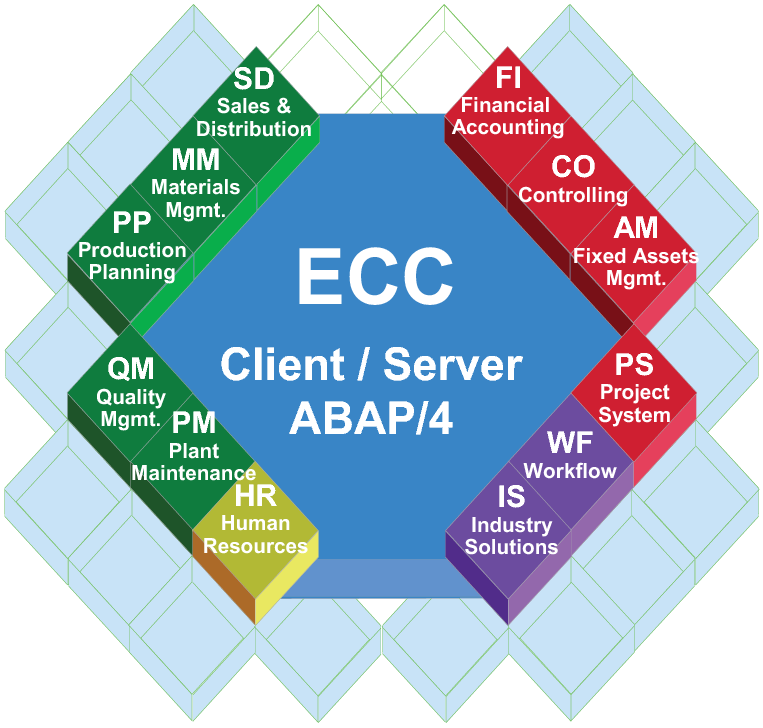
\includegraphics[width=0.75\textwidth]{images/sap_r3}
	\caption{Moduly SAP R3 \cite{sap_r3_modules}}
	\label{img:sapr3}
\end{figure}

\begin{itemize}
	\item
	\textbf{Financial Accounting (FI)}: Označuje finanční účetnictví a je jedním z nejdůležitějších modulů SAP ERP. Používá se k ukládání finančních dat organizace a pomáhá k analyzování jejího finančního postavení na trhu.
	\item
	\textbf{Controlling (CO)}: Jeho primárním účelem je plánování a následná kontrola vytvořených plánů uvnitř organizace. Podporuje koordinaci, monitorování a optimalizaci všech procesů. Zahrnuje správu a konfiguraci základních dat, které pokrývají náklady a výnosy, interní objednávky a další nákladové prvky. 
	\item
	\textbf{Asset Management (AM)}: Slouží k optimální správě fyzického majetku organizace. Zahrnuje takové funkcionality jako jsou návrh, konstrukce, provoz nebo údržba a výměna zařízení.
	\item
	\textbf{Project system (PS)}: Je nástroj pro správu dlouhodobých projektů. Umožňuje plánovat finanční prostředky i zdroje a kontrolovat jednotlivé části projektu tak, aby bylo zaručeno včasné dodání, pokud možno v rámci rozpočtu.
	\item
	\textbf{Workflow (WF)}: Umožňuje navrhovat a realizovat obchodní procesy v rámci aplikačních systémů SAP. Zajišťuje, aby se práce v požadovaný čas dostala do rukou správným lidem. Jeho cílem je usnadnění automatizace podnikových procesů.
	\item
	\textbf{Industry Solutions (IS)}: Poskytuje specifická řešení pro desítky industriálních odvětví jako například automobilový, chemický či energetický průmysl.
	\item
	\textbf{Human Resources (HR)}: Umožňuje organizaci strukturálně a efektivně zpracovávat informace týkající se zaměstnanců. Poskytuje přehled o lidských kapacitách a nástroje k jejich strategickému rozvoji.
	\item
	\textbf{Plant Maintenance (PM)}: Poskytuje nástroj pro provádění veškerých potřebných činností týkajících se údržby organizace a jejích součástí. Umožňuje plánovat údržbu i s ohledem na materiálovou potřebu, zaznamenávat a vyrovnávat náklady spojené s činností.
	\item
	\textbf{Materials Management (MM)}: Se zabývá řízením materiálů a skladových zásob. Kontroluje, aby nedocházelo k nedostatkům zboží a nevznikaly tak mezery v řetězci dodavatelského procesu.
	\item
	\textbf{Production Planning (PP)}: Sleduje a zaznamenává toky ve výrobním procesu. Má za úkol sladění poptávky s výrobní kapacitou spolu s vytvořením plánů k dokončení jednotlivých komponent a produktů.
	\item
	\textbf{Quality Management (QM)}: Je modul úzce provázaný s moduly MM, PP či PM a nedílnou součástí logistického řízení. Používá se k provádění kvalitativních funkcí jako je například vyhodnocení výkonnosti a spolehlivosti procesů, počtu reklamací od zákazníků atd. Důslednou kontrolou produktů je dosaženo vyšší spokojenosti zákazníka.
	\item
	\textbf{Sales and Distribution (SD)}: Se používá pro ukládání údajů o zákaznících a produktech organizace. Pomáhá řídit fakturaci, prodej a distribuci produktů či služeb organizace. Řídí vztah se zákazníky od počáteční nabídky až po prodejní zakázku a fakturaci produktu.   
\end{itemize} 	
Kombinací všech těchto modulů potom vzniká velmi komplexní a modulární systém, který se dá ještě rozvíjet a upravovat dle zákazníkových požadavků. Výsledkem je pak podnikový informační systém \uv{ušitý na míru}.

\section{SAP Plant Maintenance (PM)}
Modulem, který je pro tuto práci stěžejním, je modul SAP Plant Maintenance. Jedná se o komplexní řešení, které poskytuje nástroje pro údržbu strojů a vybavení v rámci celé organizace. Veškeré aktivity jsou vzájemně propojeny s návaznými moduly (Production Planning, Materials Management a Sales and Distribution) v rámci podnikových procesů. Modul umožňuje provádět plánování, realizovat denní činnosti údržby nebo zaznamenávat vzniklé problémy a poruchy. Díky provázanosti s ostatními moduly taktéž dovede sledovat a plánovat materiálové aktivity, případně určovat náklady vzniklé údržbou. K realizování všech těchto aktivit je modul rozdělen do následujících podmodulů. Hlavním zdrojem informací pro tuto část je dokument \cite{sap_pm_document} popisující většinu základních procesů v modulu PM.
\begin{itemize}
	\item
	Správa technických objektů a vybavení
	\item
	Plánování úkolů údržby
	\item
	Řízení notifikací v rámci nastavených procesů 
\end{itemize} 	

\subsection{Technické objekty}
Pro správné a efektivní provádění jednotlivých aktivit v rámci procesů modulu PM je struktura údržby rozdělena na technické objekty. Ty slouží k definování jednotlivých typů strojů, kterými organizace disponuje. S použitím charakteristiky technických objektů lze pak zadefinovat jiný technický objekt, což umožňuje hierarchické definování struktury organizace. To s sebou přináší následující výhody.
\begin{itemize}
	\item
	Doba potřebná pro správu jednotlivých technických objektů je snížena.
	\item
	Zpracování údržby je zjednodušeno.
	\item
	Konkrétnější, důkladnější a rychlejší vyhodnocení údajů o údržbě.
\end{itemize}
Klíčová funkcionalita systému se dá shrnout do následujících bodů. Jednotlivým bodům se poté věnují podrobnější podkapitoly.
\begin{itemize}
	\item
	\textbf{Inspekce}: Spočívá v měření a sledování aktuálního stavu technického objektu.
	\item
	\textbf{Preventivní údržba}: Slouží k zaručení vysoké spolehlivosti výrobního procesu. Zahrnuje plánování údržby a časování aktivit pro jednotlivé technické objekty.
	\item
	\textbf{Oprava poruchy}: Zahrnuje veškerá opatření, která jsou nutná k obnovení ideálního stavu technických objektů. Cílem je maximální eliminace prostojů ve výrobě a snížení nákladů na výrobu.
\end{itemize}

\subsection{Inspekce a preventivní údržba}
Preventivní údržba je dlouhodobý a plánovaný proces, jehož cílem je zajištění vysoké použitelnosti zařízení a minimalizování prostojů způsobovaných opravami. Pomocí preventivního chování lze potom v organizaci dosáhnout řady výhod. Dosažením maximální využitelnosti strojů lze snížit jejich počet blíže k minimu a tím tak dosáhnout menších nákladů na pořizování technologií a tím i snížení potřebných kapacit lidských zdrojů. Vybavení ve špatném stavu má negativní dopady na morálku zaměstnanců a jejich výkonnost. I to je jeden z dalších důvodů, proč je dobré mít nastavené správné preventivní procesy. Pro stanovení takového procesu lze určit řadu specifikujících parametrů. Příklady takových parametrů jsou nastíněny v následujícím seznamu.
\begin{itemize}
	\item
	Seznam úkolů, které mají být v rámci prevence provedeny
	\item
	Rozsah inspekčních a preventivních prací
	\item
	Frekvence kontroly 
	\item
	Limit nákladů spojených s preventivní údržbou
\end{itemize} 	
Seznam úkolů pro preventivní údržbu je definován jako sled činností, které jsou prováděny zodpovědnými zaměstnanci. Pomocí pevně daného seznamu úkolů lze standardizovat pracovní postupy a tím tak dosáhnout vyšší efektivnosti. V rámci systému je potom v závislosti na aktuálním čase prevence dělena na plánovanou a přetrvávající údržbu.

\paragraph{Plánovaná údržba}
Všechny plánované aktivity, jakou jsou údržba, prevence, inspekce a opravy spadají pod plánovanou údržbu. V modulu PM jim mohou být přiřazeny časové intervaly vykonávání údržby. Čas může být přidělen až na úrovni jednotlivých úkonů. Příkladem tak může být úkon pro dotažení šroubů na výrobní lince XYZ každé druhé pondělí ve 14 hodin.

\paragraph{Přetrvávající údržba}
Seznam úkonů přetrvávající údržby je založen na základě aktuálního stavu inspekce. Všechny takové, které jsou provedeny mimo regulérní rozvrh, spadají pod přetrvávající údržbu.

\paragraph{Údržba z technického hlediska}
Zpracování údržby se z technického pohledu skládá z několika fází, jejichž pořadí nemusí být striktně dodrženo. Jelikož se údržba týká plánování, předběžné kalkulace, zabezpečení dostatečného množství materiálu a případných povolení, může v případě nutného provedení údržby dojít k přeskočení některých kroků. Mohlo by totiž například dojít k nežádoucímu čekání na schválení kalkulace i v případě nutnosti opravy. Zpracování údržby lze rozdělit na následující tři oblasti:
\begin{itemize}
	\item
	\textbf{Popis stavu objektu}: Slouží k podání oznámení o údržbě, používá se k popisu stavu technického objektu nebo k nahlášení poruchy spolu s následným požadavkem na opravu.
	\item
	\textbf{Provádění úkolů údržby}: Spočívá v objednání údržby. Používá se k detailnímu plánování provádění údržbářských činností, sledování průběhu práce a vypořádání nákladů na údržbu.
	\item
	\textbf{Dokončení úkolů údržby}: Slouží zejména k zaznamenávání historie údržby. Používá se k dlouhodobému uložení nejdůležitějších údajů o údržbě, které lze následně z různých důvodů analyzovat. 
\end{itemize} 
Na následujícím obrázku \ref{img:pm_process} je zobrazen životní \textbf{cyklus požadované údržby, případně nahlášené poruchy}.
\begin{figure}[H]
	\centering
	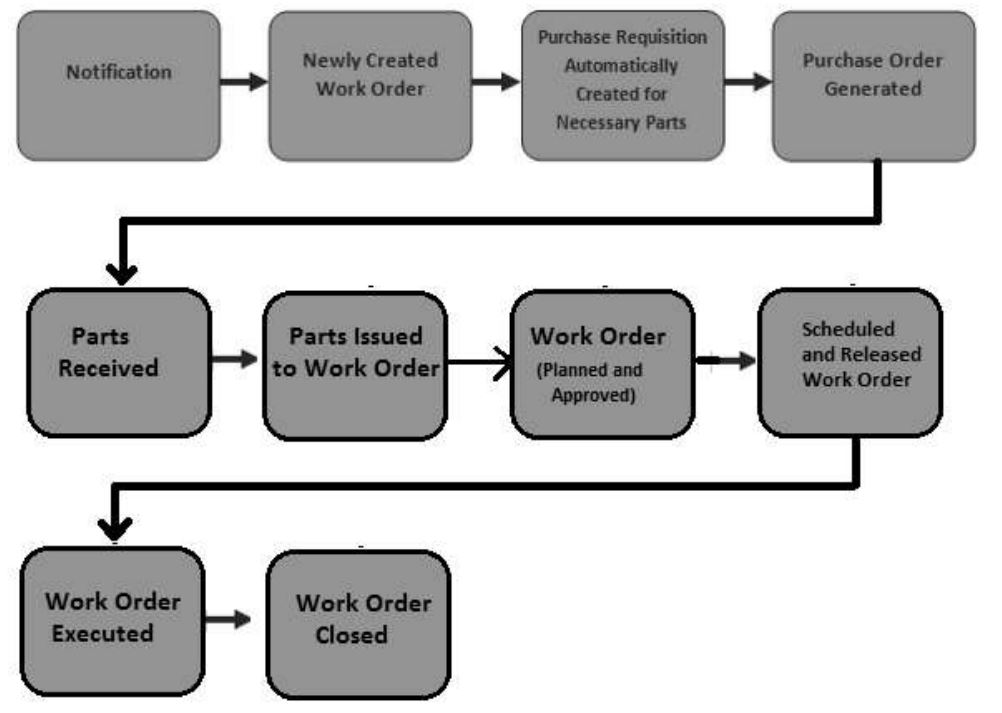
\includegraphics[width=1\textwidth]{images/pm_process.jpg}
	\caption{Proces diagram PM}
	\label{img:pm_process}
\end{figure}
V prvním kroku musí dojít k podání požadavku na údržbu. Poté technicky dojde k založení objednávky se všemi náležitostmi. Tu posléze může realizovat některý z údržbářů, který má možnost daný problém řešit. Počátkem jeho prací dojde k založení servisní zakázky, pro kterou díky propojení na ostatní moduly probíhá kalkulace nákladů. Jelikož k vyřešení problému může údržbář potřebovat různý materiál (například šrouby a matice), je v procesu zobrazeno vytvoření objednávky na vydání materiálu. Po případném vyzvednutí materiálu a dokončení údržby dojde k ukončení servisní zakázky a celého procesu údržby. závěrem je celý proces zaznamenám a finančně vyhodnocen.

Tím je popsán základní proces nad modulem PM potřebný k pochopení a následnému návrhu aplikace, která bude tento, mimo jiné, proces realizovat.

\section{SAP BSP}
\label{sec:bsp}
Tato sekce se zaměřuje na frontendovou technologii SAP BSP. Jedná se o jednu z technologií použitých v cílové architektuře řešení mobilní aplikace a proto je zde stručně popsána její struktura pro pochopení její role v celkové architektuře. 

\paragraph{BSP (Business Server Page)} Je jednou z variant, jak SAP programy a transakce zpřístupnit i mimo desktop aplikaci SAPGUI běžně používanou pro přístup do systému. Představuje funkční HTML aplikaci, u které lze dosáhnout takového chování jako u klasické SAP transakce. Tím je umožněno získat přístup do systém skrze libovolný webový prohlížeč. Na následujícím obrázku \ref{img:bsp_structure} je k vidění struktura BSP aplikace. 
\begin{figure}[H]
	\centering
	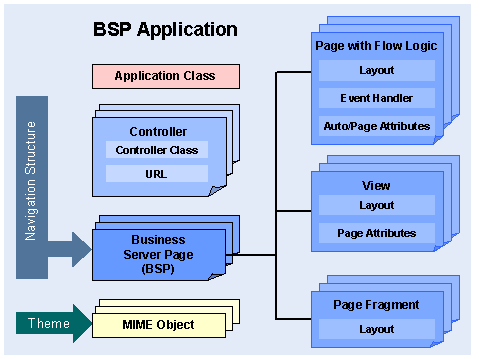
\includegraphics[width=0.75\textwidth]{images/bsp.png}
	\caption{Struktura BSP aplikace}
	\label{img:bsp_structure}
\end{figure}
Každá taková stránka se skládá z layoutu, do kterého je možné vložit standardní HTML komponenty (head, body, input a podobně). Kromě toho je možné do takové stránky vložit i kód programovacího jazyka ABAP. Tím je vytvořen silný nástroj umožňující dynamické tvoření hierarchie stránky v závislosti na získaných datech. Jelikož se jedná o HTML stránku, tak je možné v každé BSP stránce zpracovávat vstupní data. Ty jsou získány  buď pomocí metody HTTP(s) GET (informace se nese v uživateli zadané URL) nebo pomocí HTTP(s) POST (informace zakódovány v těle HTTP requestu).

Každá taková stránka má několik událostí. V následujícím výčtu jsou popsány relevantní pro vývoj požadované aplikace. 
\begin{itemize}
	\item
	\textbf{OnCreate}: Událost je vyvolána v případě prvního načtení v rámci session. Může posloužit k vytvoření potřebných tříd nebo načtení neměnných dat.
	\item
	\textbf{OnRequest}: Nejdůležitější událost z hlediska vývoje požadované aplikace. Je vyvolána při každém requestu vůči BSP aplikaci. V tento moment lze vyčíst zasílaná data a v závislosti na nich provést adekvátní operace. Příkladem může být přijetí requestu s požadavkem na detail uživatele MORMAITE. Pomocí kódu v programovacím jazyce ABAP lze z databázových tabulek vyčíst požadované informace a uživateli je nějakým způsobem zobrazit zpátky.
	\item
	\textbf{OnDestroy}: Slouží především pro uvolnění použitých prostředků. To sice není nezbytně nutné, systém to po čase provede sám. Nicméně se vůči systému jedná o nenáročnost slušnost.
\end{itemize} 

\section{SAP FIORI}
\label{sec:fiori}
Systém SAP byl po dvě desetiletí přístupný zejména prostřednictvím destop aplikace SAPGUI. Jedná se tedy o aplikaci navrženou v 90. letech 20. století a tomu odpovídá i její vzhled. Nejedná se zrovna o User-Friendly rozhraní a to si SAP management samozřejmě uvědomuje. Kromě toho se nejedná zrovna ani o nejdostupnější řešení. Proto v roce 2013 společnost SAP přišla platformou SAP Mobile Platform 3.0 startující novou éru přístupu k systému SAP. Mobilní platforma dostala obchodní název Fiori. Bylo založena na základě následujících pěti pravidlech.
\begin{itemize}
	\item
	\textbf{Založené na rolích}: Má se jednat o uživatelsky orientované aplikace závislé na rolích uživatele. Uživatel může mít více rolí a provádět tak zcela rozdílné úkoly v rámci různých aplikací.  
	\item
	\textbf{Responzivní}: Budou založené na HTML5. Musí bez problému pracovat na různých zařízeních bez ohledu na velikost obrazovky. V případě změny rozlišení musí aplikace adekvátně reagovat a přizpůsobit svůj vzhled. A nakonec musí podporovat různé režimy interakce jako jsou klávesnice, myši nebo dotykové vstupy.
	\item
	\textbf{Jednoduché}: Jednotlivé obrazovky musí být jednoduché a zobrazovat relevantní informace. Práce s aplikacemi musí být intuitivní a neměla by vyžadovat návod k zacházení.
	\item
	\textbf{Koherentní}: Napříč aplikacemi musí být zachován stejný design a princ použití. Snadno se pak uživatel sžije s novými aplikacemi poté, co už s některou Fiori aplikací pracoval.
	\item
	\textbf{Líbivé}: Aplikace se musí uživatelům líbit, motivuje je to při práci a tím snižuje náklady společnosti.
\end{itemize} 	
Zavedením této technologie má dojít k odstranění problémů s nespokojenými zákazníky ohledně staromódního vzhledu a komplikované práci. Společnost SAP od té doby vytvořila stovky Fiori aplikací, které si mohou zákazníci zakoupit. Jedná se například o aplikace pro vyřizování objednávek, správu uživatelů a mnoho dalších. 

Na následujícím obrázku \ref{img:fiori_design} je k vidění aktuální design prezentovaný společností SAP.
\begin{figure}[H]
	\centering
	
\includegraphics[width=1\textwidth]{images/fiori}
	\caption{Design Fiori aplikací}
	\label{img:fiori_design}
\end{figure}

\subsection{Technický pohled}
Frameworkem pro tvorbu Fiori aplikací je SAPUI5. Jeho základní struktura je zobrazena na obrázku \ref{img:fiori_arch} níže. Jedná se o sadu vývojářských nástrojů, které slouží k vytváření aplikací s bohatým uživatelským rozhraním pro moderní business webové aplikace. Jeho základem je JavaScript knihovna Core, která poskytuje zejména prostředky pro podporu MVC \ref{ssec:mvc} konceptu. Dále nabízí možnosti provazování dat s UI prvky z různých datových zdrojů (JSON, XML, OData \ref{ssec:odata}) a efektivní práci s jednotlivými HTML prvky. 
\begin{figure}[H]
	\centering
	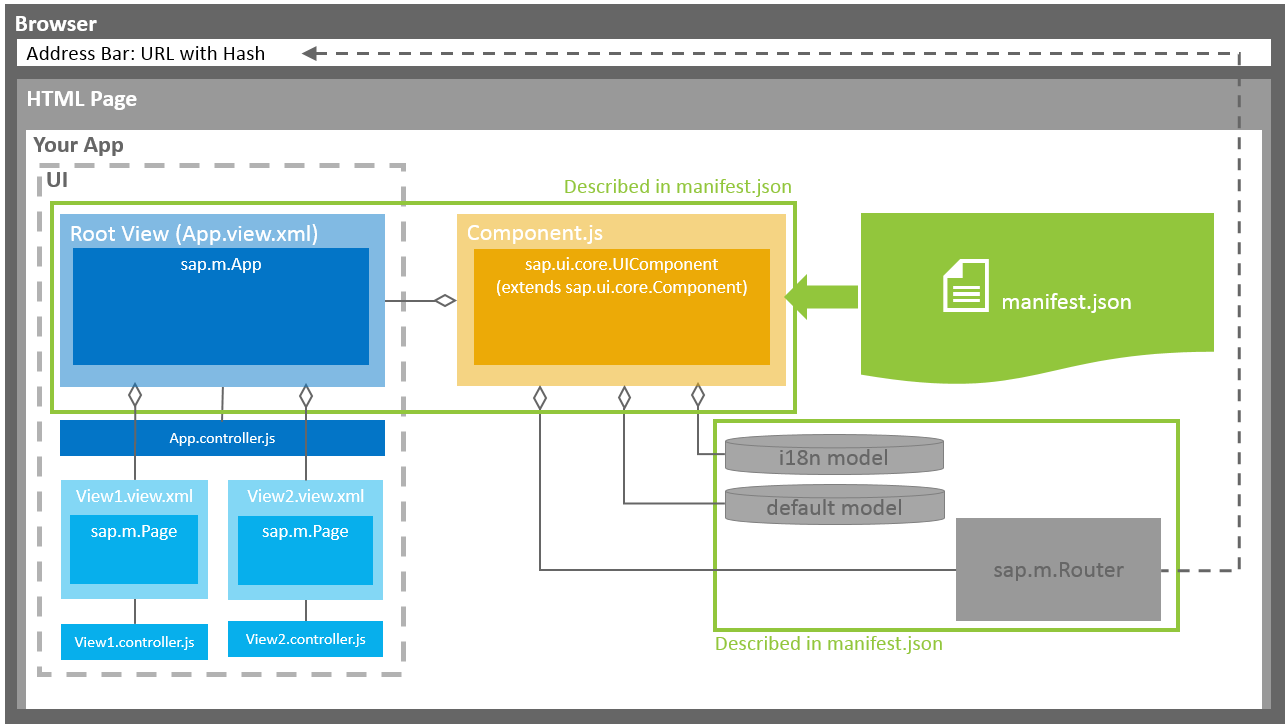
\includegraphics[width=1\textwidth]{images/fiori_arch.png}
	\caption{Struktura BSP aplikace \cite{fiori_structure}}
	\label{img:fiori_arch}
\end{figure}
Struktura frameworku spočívá především v konceptu MVC. Při zavádění aplikace dojde k vytvoření hlavní \textbf{komponenty} (Component.js), která obaluje jednotlivá \textbf{view} zadefinovaná v rámci aplikace. Pod každým view si lze představit libovolnou stránku. Každá taková stránka má přiřazen právě jeden \textbf{controller}, který reaguje a obstarává uživatelovu interakci. Klikne-li uživatel na tlačítko vymazat záznam, je to právě controller, kdo odchytí uživatelovu akci a musí na ni adekvátně zareagovat. V takovém případě by nejspíš zobrazil dialog pro potvrzení nebo rovnou poslal na backend request pro vykonání dané operace. Podrobněji se jednotlivým souborům použitým ve frameworku SAPUI5 věnuje implementační část v kapitole \ref{ssec:struckuta_pm_aplikace}.

\paragraph{UI komponenty}
Framework má k dispozici více než 200 komponent, které umožňují skládání výsledné podoby uživatelského rozhraní. Takovou komponentou může být jednoduché zobrazení textu, ale i složitý layout rozdělující stránku na několik nezávislých částí. Obsahuje spoustu typických layoutů potřebných při téměř každém vývoj aplikace. Tím může být například vstupní formulář nebo zobrazení seznamu prvků. 

\subsection{MVC}
\label{ssec:mvc}
Základem celého frameworku je návrhový vzor MVC (Model-View-Controller). Rozděluje aplikaci na tři nezávislé komponenty. Jedná se o datový mode, uživatelské rozhraní a řídící logiku. Symbolické znázornění funkčnosti vzoru je k vidění na obrázku \ref{img:mvc} zobrazeném níže.
\begin{figure}[H]
	\centering
	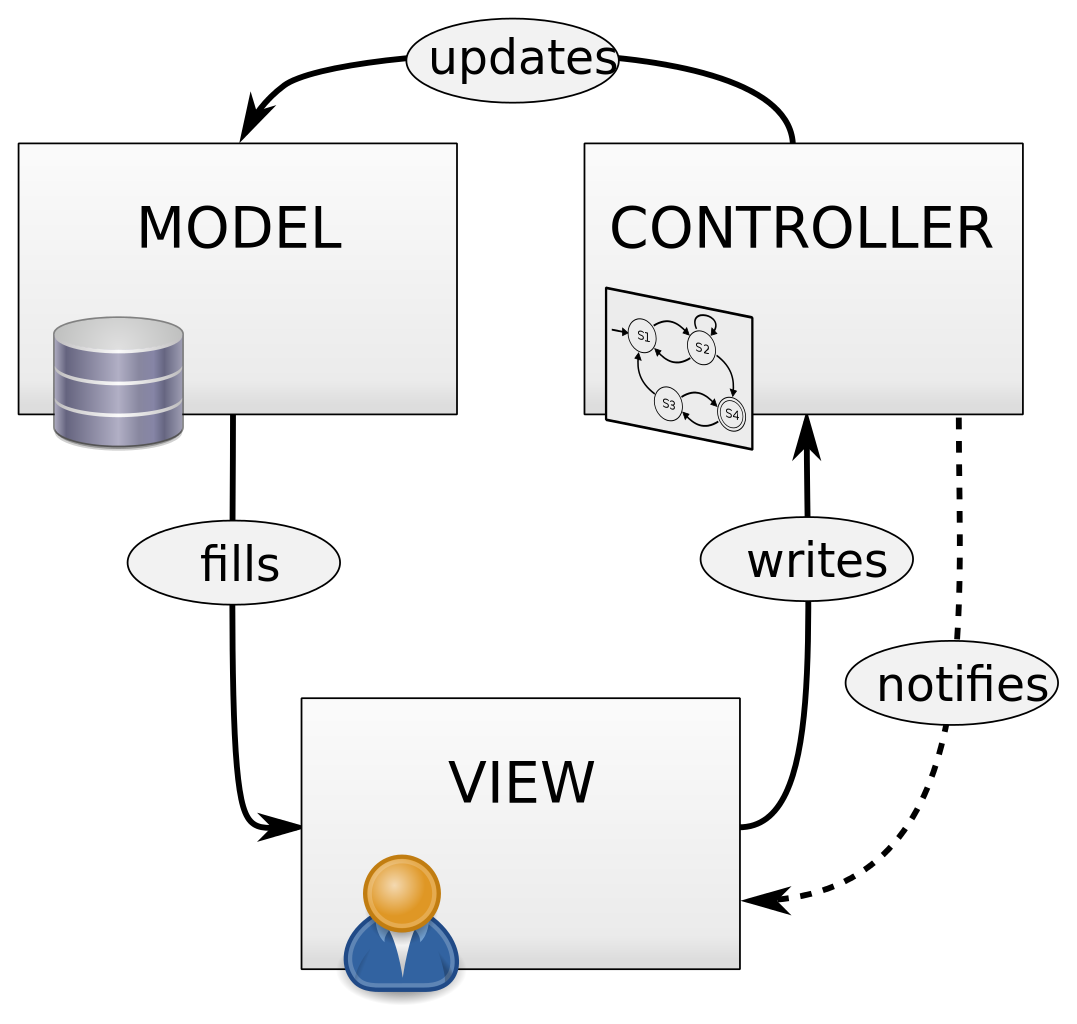
\includegraphics[width=0.5\textwidth]{images/mvc.png}
	\caption{Návrhový vzor MVC}
	\label{img:mvc}
\end{figure}
\paragraph{Model} Reprezentuje správu dat, nad nimiž aplikace pracuje. Takovými daty může být seznam uživatelů, detail objednávky nebo obrázek v binární podobě. Jelikož se z v architektonickém modelu server-klient jedná o prezentační vrstvu, je vhodné, aby data měly co možná nejpřijatelnější podobu pro prezentování uživateli. 
\paragraph{View} Zahrnuje všechny grafické objekty uživatelského rozhraní. Jedná se o komponenty, s kterými uživatel přímo pracuje. Pomocí nich mu jsou prezentovány požadovaná data v prezentovatelné formě. A naopak pouze jejich prostřednictvím uživatel dává aplikaci příkazy k provedení požadované činnosti. Výhodou jednotlivých komponent je nezávislost na modelu a controlleru. Grafické komponenty lze tak v průběhu aplikace měnit. 
\paragraph{Controller} Dělá prostředníka datovému modelu a uživatelským rozhraním. Má na starost obstarávání uživatelských akcí vůči rozhraní. Klikne-li uživatel na tlačítko, je právě na něm, aby provedl adekvátní akci očekávanou od uživatele. Upravuje data uložená v modelu, čímž může měnit uživateli prezentovaná data. A taktéž může zasahovat do view jako takového. V případě, že je zapotřebí některé elementy schovat nebo naopak zobrazit, je to právě controller, kdo může takovou akci provést.

\subsection{SAP ODATA}
\label{ssec:odata}
Protokol OData umožňuje vytváření datových služeb založených na webovém protokolu REST (Representational State Transfer), který umožňuje uživatelům provádět CRUD (Create, Read, Update, Delete) operace nad zdroji identifikovanými pomocí URI (Uniform Resource Identifier) a definovanými v datovém modelu použitím HTTP requestů.

Data přenášená prostřednictvím OData protokolu mohou využívat různé datové formáty běžně používané ve webových technologiích. Příkladem  může být XML (Extensible Markup Language), JSON (JavaScript Object Notation) nebo další. Data jsou při přenosu zabalena do protokolu HTTP, případně do jeho zabezpečené verze HTTPS.

Jádrem OData jsou feeds, které jsou kolekcemi Collections složené ze záznamů Entries. Každý Entry je identifikovaný klíčem a reprezentuje strukturovaný záznam, který má seznam vlastností Properties, ty mohou být komplexního, nebo primitivního typu. Entries mohou být součástí hierarchie typů a mohou mít související entries a feeds odkazované prostřednictvím Links \cite{mvc}.

\paragraph{EDM (Entity Data Model)} Hlavním konceptem v EDM jsou entity a asociace. Entita je strukturovaný záznam představující libovolný datový objekt. Tím může být například uživatel nebo objednávka. Každá taková entita má svůj klíč, kterému se říká klíč entity. Pomocí tohoto klíče lze asociovat entity mezi sebou. Budeli objednávka přiřazena k nějakému uživateli, bude mít klíč uživatele u sebe dostupný. Namapováním klíče uživatele na objednávky obsahující jeho klíč dostaneme asociaci uživatelovi objednávky. Takto lze hierarchicky libovolně navazovat asociace na jiné a tím tak vytvářet požadované datové struktury připravené k exportu. 

\paragraph{JSON (JavaScript Object Notation)}
\label{par:json}
Jedná se o datový formát velmi často využívaný ve frameworku SAPUI5 a je i jednou z podob, ve které lze prezentovat OData. Jedná se o nezávislou datovou reprezentaci, jejíž základní prvek je objekt, který může být:
\begin{itemize}
	\item
	Reálnou hodnotou (číslo, text, boolean hodnota true/false nebo null)
	\item
	Struktura objektů
    \item
	Pole objektů	
\end{itemize} 

Jedná se tak o velmi striktní, ale jednoduchou definici objektu. Postupným skládáním jednotlivých objektů do sebe lze vytvořit neomezenou hierarchickou strukturu. Na obrázku \ref{img:json} níže je zobrazena ukázková struktura JSON objektu.

\begin{figure}[H]
	\centering
	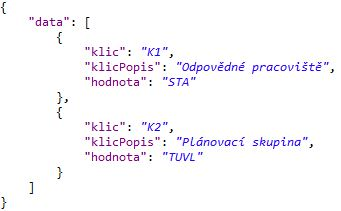
\includegraphics[width=0.5\textwidth]{images/json}
	\caption{Ukázka JSON Objektu}
	\label{img:json}
\end{figure}

JSON je textový, na jazyce zcela nezávislý formát, využívající však konvence dobře známé programátorům jazyků rodiny C (C, C++, C\#, Java, JavaScript, Perl, Python a dalších). Díky tomu je JSON pro výměnu dat opravdu ideálním jazykem \cite{json}.


% % % % % % % % % % % % % % % % % % % % % % % % % % % % % % % % % % % % % % % % % % % % % % % % % % % % % % % % % % % % 

\chapter{Analýza}
\label{chap:analyza}
Tato kapitola se věnuje analýze a návrhu požadované webové aplikace pracující nad modulem SAP Plant Maintenance pro vykonávání údržby. Jednotlivé podkapitoly se pak zaobírají zpracováním požadavků kladených na výslednou funkcionalitu. Dále jsou zde nadefinována omezení aplikace a uživatelské role, které budou v aplikaci použity. Na základě stanovených požadavků je posléze proveden návrh uživatelského rozhraní. Postupy aplikované v této kapitole vychází z přednášek a doporučení popsaných v přednáškách předmětu Softwarového inženýrství \cite{edux_si}. 

\section{Základní popis aplikace}
Webová aplikace bude svým uživatelům umožňovat vykonávat potřebné úkony pro bezproblémový chod výrobních hal. To zahrnuje důležité operace jako je například hlášení požadavků na údržbu nebo případných poruch. Takovou poruchu lze nahlásit na konkrétní vybavení nacházející se na pracovišti. Musí zaměstnancům zodpovědným za údržbu umožňovat evidování práce na nahlášených poruchách. Podrobný soupis funkčních požadavků je popsán v následující kapitole. 

\section{Uživatelské role}
\label{sec:role}
Uživatelské role popsané v této sekci jsou vytvořeny na základě požadavků v kapitole \ref{sec:model_pozadavku}. Ovšem pro jejich lepší čitelnost jsou popsány již zde. 
\subsection{Údržbář}
\label{ssec:udrzbar}
Uživatel, který primárně řeší plánované údržby z preventivních důvodů. Tím může být například periodicky v modulu PM nastavená kontrola výrobní linky. Jeho povinností je řešení nahlášených požadavků na údržbu nebo poruch.
\subsection{Operátor výroby}
\label{ssec:operator_vyroby}
Uživatel, jehož primárním účelem je obsluha strojů na jemu přiděleném pracovišti ve výrobním procesu. S aplikací přijde do styku pouze v případě, když bude chtít nahlásit poruchu vybavení v jeho pracovní sekci. Jednotlivá pracoviště jsou vybavena stolními počítači, na kterých jsou spuštěny aplikace potřebné pro provoz. Z těchto aplikací bude umožněna navigace do budoucí webové aplikace pro nahlášení případného problému.
\subsection{Uživatel s možností založení požadavku na údržbu}
\label{ssec:pozadavek_udrzba}
Uživatel, jehož zodpovědností je bezproblémový chod strojů. Osoba by se dala charakterizovat jako revizní technik, který má na starost obcházení všech pracovišť a kontrolu jednotlivých výrobních linek. V případě, že shledá za vhodné provést na nějakém stroji údržbu, založí adekvátní požadavek. Tento úkon se bude zpravidla provádět z přenosného zařízení, které má pracovník neustále u sebe. Tím může být například chytrý telefon nebo tablet.
\subsection{Správce - administrátor}
\label{ssec:administrator}
Uživatel zodpovědný za správu ostatních uživatelských účtů. Pomocí rolí bude definovat možnosti jednotlivých uživatelů. Jelikož role nejsou uživatelsky výlučné, budou mít dvě fyzické osoby představující údržbáře možnost provádět jiný okruh úkonů. Oba dva budou moci například vykonávat údržbářské činnosti, ale jenom jeden z nich bude moci zakládat požadavky na údržbu.

\section{Model požadavků}
\label{sec:model_pozadavku}
V této sekci jsou uvedeny veškeré požadavky kladené na výslednou aplikaci, které byly probírány se zadavatelem. Požadavky představují minimální kritéria potřebná pro samotný návrh uživatelského rozhraní. Veškeré požadavky byly probírány se zadavatelem, většina z nich byla jasně stanovena v rámci rámcového zadání, některé však byly lehce v rámci konzultací během vývoje aplikace. Cíle při vytváření kteréhokoli modelu požadavků jsou vypsány v následujícím výčtu.
\begin{itemize}
	\item
	\textbf{Vymezení hranic aplikace}: Slouží ke stanovení oblastí, pro kterou bude aplikace sloužit. Příkladem takové hranice nad modulem PM může být práce pouze pro zakládání požadavků na údržbu a poruch. Od takové aplikace se potom nebude očekávat správa technického vybavení.
	\item
	\textbf{Odhad pracnosti}: Za pomocí stanovené funkcionality a ostatních požadavků je mnohem jednodušší stanovit odhad celkové pracnosti. nad seznamem jednotlivých funkcionalit se provede jednodušší odhad a rezerva potřebná pro vývoj.
	\item
	\textbf{Vyjasnění zadání}: Ne vždy bohužel zákazník dobře ví, co vlastně od aplikace očekává. Proto je dobré si s ním dané funkcionality prodiskutovat a následně pevně stanovit.
	\item
	\textbf{Zachycení omezení}: Slouží k předejití fatálních problémů při vývoji. Je zapotřebí zabránit problémům, které se například až v době nahrávání aplikace do produktivního prostředí, protože je zde pro server použita jiná verze operačního systému nebo jsou zde problémy s oprávněním a přístupem do internetu.
\end{itemize} 
Jednou z pomůcek pro dobré definování cílů aplikace je technika \textbf{SMART}. Ta popisuje vlastnosti cílů pomocí následujícího výčtu \cite{edux_pcm1}. 
\begin{itemize}
	\item
	\textbf{S (Specific)}: Musí být definován přesně. Čím přesnější cíl bude, tím snadněji bude docházet k jeho implementaci a předejde se tak možným nedorozuměním. Obecně platí, že to, co je jasné jednomu člověku nemusí být pochopeno na opačné straně stejně. 
	\item
	\textbf{M (Measurable)}: Aby bylo možné dosažení cílů posoudit, měli by být dobře měřitelné.
	\item
	\textbf{A (Accepted)}: K akceptaci musí dojít odpovědnou osobou. Dokud nebude mít tým potvrzený cíl, tak si jednotliví členově vždy najdou něco \uv{zajímavějšího} na práci.
	\item
	\textbf{R (Realistic)}: Měli by být uskutečnitelné v reálném čase. Pevně stanovený termín je sice nezbytný, nicméně by se nemělo jednat o nesplnitelný termín. Ten by mohl pracovní morálku týmu jenom zhoršit.
	\item
	\textbf{T (Timed)}: Časové omezení je nezbytně nutné. Pokud nebude jasně stanoven termín dodání bude mít tendenci jednotlivé úkony odkládat.
\end{itemize} 

\subsection{Funkční požadavky}
\label{ssec:funkcni_pozadavky}
Jsou takové požadavky, které musí být ve výsledné aplikaci implementovány tak, aby byla splněna očekávaná funkcionalita. Požadavky jsou rozděleny do sedmi sekcí označených jako F1 až F7. Jedná se především o funkcionality spojené s nahlašováním poruch nebo požadavků na údržbu společně s úkony prováděných nad již vzniklými hlášeními. 
\subsubsection{F1: Založení požadavku na údržbu}
\label{sssec:fc_zalozeni_pozadavku}
V případě zjištění potřeby údržby daného vybavení bude uživateli s oprávněním tuto činnost provádět k dispozici založení hlášení v modulu PM s následující editovatelnými parametry.
\begin{itemize}
	\item
	\textbf{Vybavení}: Výběr bude umožněn pomocí hierarchické struktury představující podobu závodu. V případě, že bude uživateli přednastaveno výchozí technické místo (například pracovní linka), bude výběrová struktura příslušně omezena. Provedení výběru by mělo být v mobilním zařízení umožněno i pomocí naskenování QR kódu.  
	\item
	\textbf{Příloha}: Ke každému požadavku bude umožněno přiložené jedné přílohy s tím, že prozatím bude omezeno pouze na fotografie (omezený výčet typů souborů). Do budoucna se počítá s rozšířením na vyšší počet příloh.  
	\item
	\textbf{Priorita}: Stanovuje termín, do kterého se očekává provedení požadované údržby nebo opravy. Řešeno pomocí tří úrovní důležitosti, podle kterých se očekává zpracování požadavku v horizontu dne, týdne nebo měsíce.
	\item
	\textbf{Plánovací skupin}: Spočívá ve výběru subjektu zodpovídajícího za údržbu. Fyzicky se jedná o skupinu lidí spravující vymezený okruh údržby (například elektromechanici, mechanici nebo revizní technici). V případě, že bude uživateli přednastavena výchozí plánovací skupina, dojde automaticky k jejímu předvyplnění.
	\item
	\textbf{Pracoviště}: Reprezentuje skupinu údržbářů, kteří jsou podřízeni příslušnému mistru údržby. Z důvodu propojení s modulem CO dochází s návazností na pracoviště k ocenění prováděné práce, která je vykazována pomocí zpětného hlášení daným pracovištěm na zakázku PM. 
	\item
	\textbf{Popis poruchy}: Jedná se o stručný popis hlášení, který jasně přibližuje daný problém. Tím může být například došlý materiál nebo opotřebení šroubu. 
\end{itemize} 
Parametry, které uživatel nebude svévolně volit jsou následující.
\begin{itemize}
	\item
	\textbf{Typ hlášení}: Vychází z prováděné operace, je stanoven konstantou určující typ hlášení požadavku na údržbu.
	\item
	\textbf{Závod}: Je definován přihlášeným uživatelem. Každý uživatel bude mít nějaký závod přidělený, jedná se o potřebný údaj při zakládání hlášení.
\end{itemize} 
Typickými uživateli využívající tento funkční požadavek budou mistři, vedoucí směn a údržbáři.
\subsubsection{F2: Nahlášení poruchy}
\label{sscec:fc_nahlaseni_poruchy}
Jelikož se technicky na úrovni modulu PM jedná o stejný záznam jako při zakládání požadavku na údržbu (rozdílná konstanta typu hlášení), je seznam potřebných parametrů stejný. Nicméně jelikož se hlášení poruchy reálně očekává od jiného typu uživatelů, je zadání hodnot u následujících parametrů trochu odlišné. Typicky totiž bude poruchu nahlašovat pracovník ve výrobě, který má přidělené své pracovní místo a spolu s tím omezené možnosti zadávání. 
\begin{itemize}
	\item
	\textbf{Vybavení}: Jelikož se očekává mnohem menší počet vybavení, které bude umožněno uživateli vybrat, nebude se provádět výběr z hierarchické struktury technických míst, ale bude k dispozici jenom takové vybavení, které spadá pod určité pracoviště. Hierarchické uspořádání však zůstane zachováno. Provedení výběru by mělo být v mobilním zařízení umožněno i pomocí naskenování QR kódu.
	\item
	\textbf{Plánovací skupin}: Uživatel bude mít na výběr hlášení poruch dvojího typu. Bude na něm, jestli si vybere poruchu s mechanickou nebo elektrotechnickou příčinou. V závislosti na tom bude plánovací skupina přednastavena z uživatelského nastavení.
\end{itemize} 
Needitovatelné parametry budou stejně jako při zakládání požadavku na údržbu přednastaveny z uživatelského nastavení.
\subsubsection{F3: Správa poruch}
\label{sssec:fc_sprava_poruch}
Uživateli musí být k dispozici seznam poruch obsahující potřebné informace (popis hlášení, technické místo spolu s vybavením, pracoviště a informace o tom kdo a kdy poruchu nahlásil včetně statusu daného hlášení) pro správné zacházení s nimi. Uživateli budou nad jednotlivými poruchami umožněny následující operace. Některé z nich jsou k dispozici v závislosti na stavu (statusu) hlášení.
\begin{itemize}
	\item
	\textbf{Evidence práce na poruše}: Údržbář (člověk s oprávněním provádět opravy) může na konkrétní poruše zahájit práci. To je technicky realizováno založením PM zakázky, u které díky integraci na modul CO dochází k evidenci nákladů. Takový uživatel může poté práci na svojí zakázce ukončit.
	\item
	\textbf{Zrušení hlášení}: V případě založení poruchy (status odpovídající stavu právě založeno) je umožněno hlášení zrušit. To například pro nevhodné nebo nechtěné založení. 
	\item
	\textbf{Vyřešení poruchy}: Poté, co se poruše začal někdo věnovat (zahájil na ní práci a tím došlo k založení zakázky PM), svou práci následně ukončil a nikdo jiný už na ní nepracuje, je možné poruchu ukončit. Poté bude údržbář vyzván k odborné specifikaci poruchy. Dostane za úkol specifikovat postiženou část objektu, typ poškození a příčinu. V takovém případě dojde k ukončení celého procesu a dané hlášení již v seznamu poruch nebude dostupné.
	\item
	\textbf{Výdej náhradního dílu ze skladu}: Pro provedení této činnosti se uživateli přednastaví z uživatelského nastavení závod a sklad s tím, že sklad bude moci případně změnit. Materiál, množství a možnost navrácení materiálu poté uživatel zadá ručně. Potvrzením zadaných parametrů dojde k vyskladnění požadovaného materiálu ze skladu.
	\item
	\textbf{Správa akcí}: Hlášení mají jasný výčet operací, které při práci s poruchou může údržbář provést. Jedná se například o informaci objednání náhradního dílu nebo požadovaného servisu. K takové akci pak může dotyčný uživatel dodat vlastní poznámku. Tyto akce mohou být zakládány, ale i zpětně prohlíženy.
	\item
	\textbf{Zobrazení textů}: Ke každému hlášení je pomocí dlouhých textů (speciální technický objekt pro ukládání řetězců neomezené délky) v SAP umožněno přidávat poznámky. V rámci hlášení bude všem dostupná historie těchto poznámek, přidávání bude umožněno v závislosti na typu uživatele.
	\item
	\textbf{Zobrazení přílohy}: V důsledku možnosti přidávat přílohu při zakládání poruchy je i v případě práce s poruchou umožněno si danou přílohu zobrazit a eventuálně stáhnout na lokální disk.
\end{itemize} 
\subsubsection{F4: Správa požadavků na údržbu}
\label{sssec:fc_sprava_poz_udr}
Uživateli musí být k dispozici seznam požadavků obsahující potřebné informace (popis požadavku, technické místo spolu s vybavením, pracoviště, mezní zahájení spolu s ukončením a informace o tom, kdo požadavek založil včetně statusu daného hlášení) pro správné zacházení s nimi. Uživateli budou umožněny stejné operace jako pří správě poruch \ref{sssec:fc_sprava_poruch}, kromě změn v následujícím seznamu. Vyřešení poruchy ze správy poruch se požadavků na údržbu netýká.
\begin{itemize}
	\item
	\textbf{Provedení údržby}: Údržbář může na konkrétním požadavku zahájit práci. Ta je technicky realizována založením PM zakázky, u které díky integraci na modul CO dochází k evidenci nákladů. Po ukončení prací na daném požadavku se bude moci údržbář rozhodnout, zdali je údržba provedena dostatečně a může tak dojít k předání hlášení operátorům výroby pro schválení. 
	\item
	\textbf{Akceptace údržby}: Operátor výroby může rozhodnout o dostatečném provedení údržby daného stroje. V takovém případě dojde k ukončení celého procesu a dané hlášení již v seznamu požadavků na údržbu nebude dostupné.
	\item
	\textbf{Reklamování údržby}: Operátor výroby může rozhodnout o nedostatečném provedení údržby daného stroje. V takovém případě dojde k navrácení hlášení údržbářům tak, aby mohli na dané údržbě znovu pracovat.
\end{itemize} 
\subsubsection{F5: Správa prevencí}
\label{sssec:fc_sprava_prev}
Uživateli musí být k dispozici seznam prevencí obsahující potřebné informace (popis prevence, technické místo spolu s vybavením, pracoviště, mezní ukončením a informace o statusu daného hlášení) pro správné zacházení s nimi. Uživateli budou umožněny stejné operace jako pří správě požadavků na údržbu \ref{sssec:fc_sprava_poz_udr}, kromě toho, že provedení údržby může provést jak údržbář, tak operátor výroby. 
\subsubsection{F6: Zobrazení dokumentace ke stroji (vybavení)}
\label{sssec:fc_zobrazeni_dokumentace}
V závislosti na vybraném technickém místě nebo vybavení dojde k zobrazení seznamu přiložené dokumentace. Ta je uložena na sdíleném uložiti v interní síti společnosti a bude tedy dostupná pouze v případě použití aplikace uvnitř dané sítě. Výběr technického místo nebo vybavení bude umožněn z hierarchické struktury.
\subsubsection{F7: Administrace uživatele}
\label{sssec:fc_administrace}
Bude umožněna obecná správa účtu uživatelů, tedy základní operace jako přidání nebo odebrání účtu, nastavení jména uživatele a osobního čísla odpovídajícímu identifikátoru zaměstnance v ERP. Administrátorský účet bude moci měnit nastavení ostatních účtů, bude přiřazovat uživatelské role (oprávnění k zacházení s jednotlivými funkcionalitami) a parametry charakterizující daného uživatele. Pod tím se schovává nastavení závodu, plánovací skupiny, předdefinovaného technického místa a dalších atributů ulehčujících uživateli práci s aplikací (například přednastavené hodnoty pro výběr pracovišť, plánovacích skupin při zakládání požadavků na údržbu nebo hlášení poruch). V případě ztráty uživatelova hesla, bude z administrátorského účtu umožněno inicializování hesla daného uživatele.

\subsection{Nefunkční požadavky}
Jsou takové požadavky, které nejsou přímo nutné pro splnění požadované funkcionality, nicméně vhodné pro správný chod aplikace. Jedná se například o specifikaci očekávání od designu, zabezpečení nebo dostupnosti systému a dalších pasivních vlastností. Navržené požadavky pro výslednou aplikaci jsou rozděleny do čtyř sekcí označených jako N1 až N4.
\subsubsection{N1: Grafické uživatelské rozhraní}
Uživatelské rozhraní bude dostupné v českém jazyce. Nicméně pro budoucí plánované využití i v zahraničních závodech se očekává snadné rozšíření do ostatních jazyků jako je například angličtina nebo němčina. Jelikož se nejedná o první organizační aplikaci pracující nad nějakým z modulů SAP, požaduje se zachování stejného UI frameworku SAPUI5.
\subsubsection{N2: Dostupnost}
Aplikace musí být viditelná v internetu, musí být tedy dostupná z veřejné internetové adresy. Aplikace musí být ovšem plně funkční i ve vnitřní síti, která nemá přístup do internetu. Veškeré zdroje aplikace musí bý tedy uloženy na interním serveru poskytujícího run-time prostředí pro webovou aplikaci.
\subsubsection{N3: Spolehlivost a spravovovanost}
Aplikace bude umožňovat logování činnosti uživatelů z důvodu lepší identifikaci chyb. A to minimálně z počátku provozu aplikace. Taktéž bude i v případě vyššího zatížení systému zajištěno požadováno dokončení transakčních kroků prováděných uživatelem.
\subsubsection{N4: Bezpečnost}
Z bezpečnostních důvodů musí v aplikaci docházet k autentizaci a autorizaci každého uživatele. Uživatel bude v aplikaci smět dělat pouze ty úkony, které mu administrátor povolí. Komunikace napříč komponentami musí být šifrována.

\section{Model případů užití (Use Case Model)}
Jedná se o detailní specifikaci funkčních požadavků. Typicky slouží pro tvorbu uživatelské příručky, jako jsou podklady k tvorbě akceptačních testů, zpřesnění odhadů pracnosti nebo zadání pro programátora. Zahrnuje informace o tom, kdo bude se systémem pracovat a jaké funkcionality kdo bude využívat. K tomu slouží vydefinovaný seznam účastníků a diagramy případů užití.

\subsection{Seznam účastníků}
\label{ssec:seznam_ucastniku}
Níže zmínění účastníci odpovídají standardnímu pracovnímu modelu stanovenému v organizaci a navrženým uživatelským rolím v kapitole \ref{sec:role}.
\begin{itemize}
	\item
	\textbf{Údržbář}: Odpovídá navržené roli údržbář \ref{ssec:udrzbar}, zpravidla bude disponovat i rolí pro zakládání požadavků na údržbu. Je zodpovědný za eliminaci nahlášených poruch a provádění nahlášené údržby jednotlivého vybavení.
	\item
	\textbf{Operátor výroby}: Vychází z navržené uživatelské role operátor výroby \ref{ssec:operator_vyroby}. Na přiděleném pracovišti provádí svoji přidělenou výrobní činnost a v aplikaci mu bude umožněno především hlásit vzniklé poruchy a zakládat požadavky na údržbu vybavení. 
	\item
	\textbf{Správce / Administrátor}: Vychází z navržené uživatelské správce / administrátor \ref{ssec:administrator}. Zodpovídá za správné nastavení uživatelských účtů.
\end{itemize} 	
Nicméně nic administrátorovi nebrání tomu role různě kombinovat, nemají mezi sebou totiž výlučný vztah. Administrátor může mít klidně i role údržbáře a operátora výroby, čímž je schopen provádět jim přiřazené operace.

\subsection{Diagram případů užití}
Slouží pro detailní specifikaci požadavků na systém s tím, že graficky zobrazuje účastníky a jejich příslušná oprávnění. V následujících podkapitolách jsou vytvořeny diagramy pro nejdůležitější procesy očekávané d výsledné aplikace.
\label{ssec:diagram_pripadu_uziti}
\subsubsection{UC1: Správa poruch}
\label{sssec:uc_sprava_poruch}
Následující případ užití týkající se správy poruch zahrnuje funkční požadavky pro hlášení poruch \ref{sscec:fc_nahlaseni_poruchy} a jejich následnou správu \ref{sssec:fc_sprava_poruch}.
\begin{figure}[H]
	\centering
	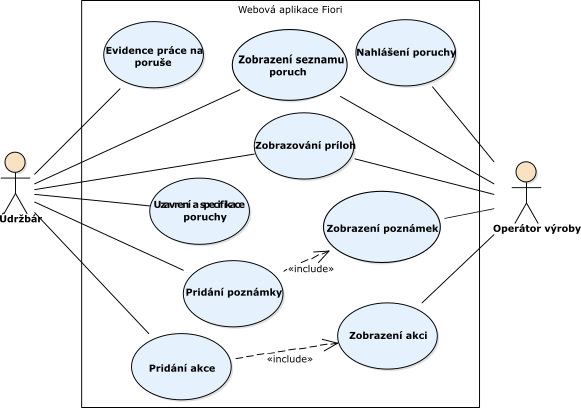
\includegraphics[width=1\textwidth]{images/ea_sprava_poruch}
	\caption{Diagram případu užití pro správu poruch}
	\label{img:uc_poruchy}
\end{figure}
V diagramu je vidět, jak jsou jednotlivé funkcionality mezi údržbáři a operátory výroby provázány. Příkladem může být nutnost zobrazení příslušného seznamu poruch. Dále je zde například vidět, že oba typy uživatelů mohou k hlášením přidávat texty a zobrazovat nad nimi provedené akce. Ovšem pouze údržbář k takovým akcím může přidat novou.

Zásadním rozdílem je ovšem možnost poruchu založit a vyřešit. Nahlášení poruchy spadá do kompetence operátora výroby a vyřešení společně s následnou specifikací poruchy do kompetence údržbáře.
\subsubsection{UC2: Správa požadavků na údržbu}
\label{sssec:uc_sprava_udrzby}
Následující případ užití se týká správy požadavků na údržbu. Zahrnuje funkční požadavky pro zakládání požadavků \ref{sssec:fc_zalozeni_pozadavku} a jejich následnou správu \ref{sssec:fc_sprava_poz_udr}.
\begin{figure}[H]
	\centering
	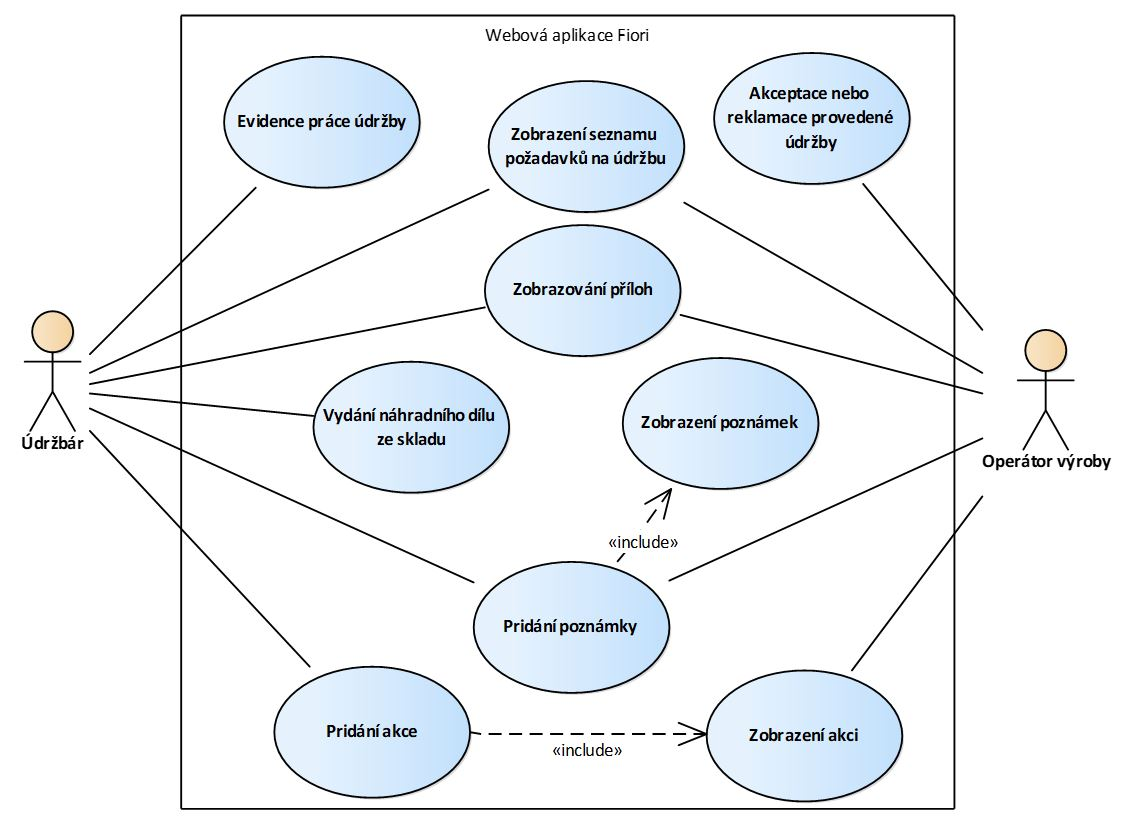
\includegraphics[width=1\textwidth]{images/ea_sprava_udrzby}
	\caption{Diagram případu užití pro správu požadavků na údržbu}
	\label{img:uc_pozadavky}
\end{figure}
V diagramu je vidět přiřazení jednotlivých funkcionalit uživatelům. Příkladem může být přidělení možnosti založení požadavku na údržbu pouze operátorovi výroby. Ten má taktéž přidělenou možnost akceptace nebo reklamace práce provedené údržbářem. Dále je zde například vidět, že oba typy uživatelů mohou k hlášením přidávat texty a zobrazovat nad nimi provedené akce. Ovšem pouze údržbář k takovým akcím může přidat novou. 
\subsubsection{UC3: Správa prevencí}
\label{sssec:uc_sprava_prevenci}
Následující případ užití se týká správy prevencí a příslušného funkčního požadavku \ref{sssec:fc_sprava_prev}.
\begin{figure}[H]
	\centering
	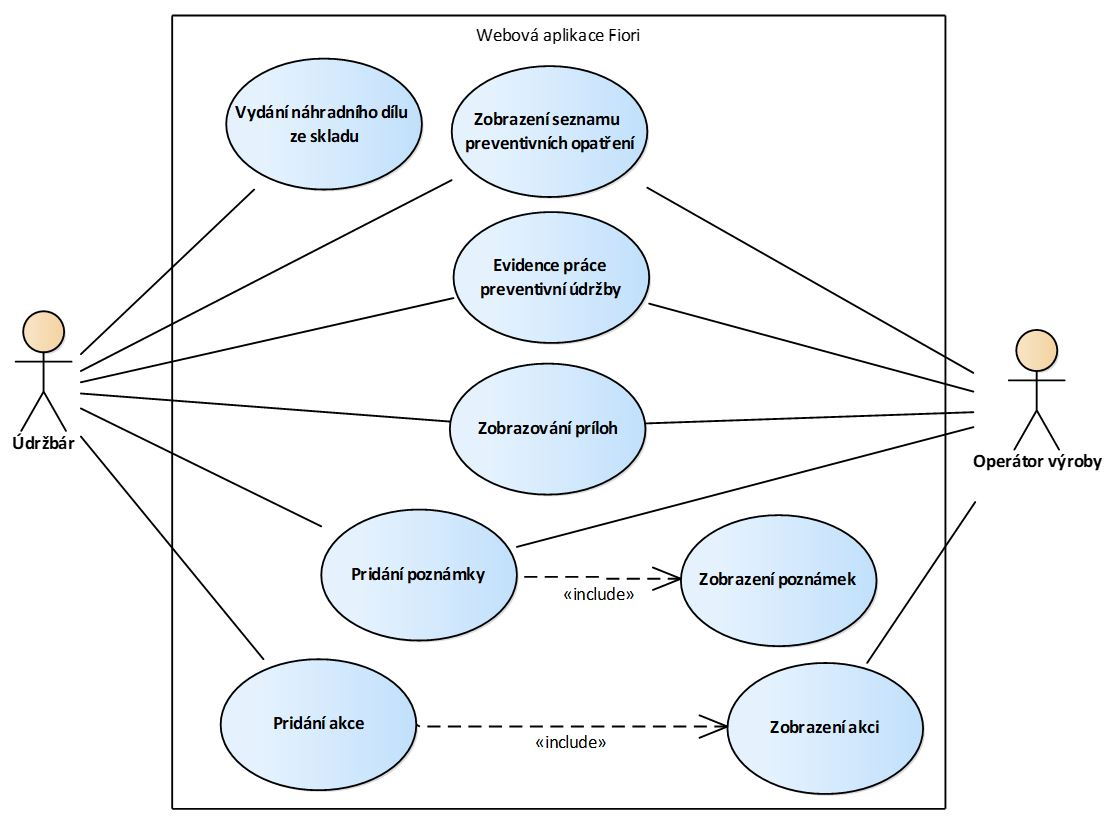
\includegraphics[width=1\textwidth]{images/ea_sprava_prevenci}
	\caption{Diagram případu užití pro správu prevencí}
	\label{img:uc_prevence}
\end{figure}
Na rozdíl od předchozích dvou případů užití \ref{sssec:uc_sprava_poruch} a \ref{sssec:uc_sprava_udrzby} může preventivní údržbu provést jak údržbář, tak i operátor výroby. To s sebou přináší i možnost zadávání akcí pro operátora výroby. Nicméně provést výdej potřebného materiálu ze skladu může stále pouze údržbář. 
\section{Závěry analýzy}
\label{sec:zav_analyzy}
Hlavním výstupem celé analýzy je rozdělení aplikace do čtyř komponent odpovídajícím uživatelským rolím. Realizování jedné společné komponenty, která by byla sdílena všemi uživateli by s sebou přinášela velké množství komplikací odpočívajících v ošetřování rolí a podmínek, kde se která operace může provést. Rozdělením sice vznikne potřeba realizovat stejné funkcionality na více místech, ale řešení pro tento problém je popsáno v kapitole \ref{chap:implementace} týkající se implementace.

% % % % % % % % % % % % % % % % % % % % % % % % % % % % % % % % % % % % % % % % % % % % % % % % % % % % % % % % % % % % 

\chapter{Návrh uživatelského rozhraní}
Tato kapitola se věnuje průběhu vytváření návrhu uživatelského rozhraní výsledné aplikace. Na základě funkčních požadavků vzešlých z prvních schůzek se zadavatelem a modelu případu užití jsou jednotlivé vzniklé úkony sdruženy v task group. Na základě task group je vytvořen task graph, který v grafické podob přiřazuje funkcionality k navrženým obrazovkám. Na základě toho je zde vytvořen Lo-Fi prototyp. K tomu byly použity dva nástroje Built.me a Balsamiq Mockups, které jsou následně porovnány. Na základě výsledků z testování Lo-Fi prototypu s uživateli jsou odpovídající změny zaneseny do výsledné aplikace. Postup použitý pro návrh uživatelského rozhraní a metody ověření jeho správnosti vycházejí z přednášek předmětu Návrh uživatelské rozhraní \cite{nur}

V první fázi je doporučováno pospat business očekávání a případy užití. Ty jsou ale již zahrnuty v rámci kapitoly \ref{chap:analyza} věnující se analýze. Proto je zde rovnou k přistoupení dalšímu kroku a to Task Groups.

\section{Task Groups}
\label{sec:task_groups}
Jsou založeny na \textbf{seznamu operací (Task List)}, které lze v rámci aplikace provést. Prvek takového seznamu může být přidání atributu uživatele nebo schválení provedené údržby. Granularita a důležitost jednotlivých položek pak může být, a zpravidla bývá, proměnná. Základním pravidlem pro tvorbu takového seznamu je rčení \uv{Don't think too much, just list the tasks}, tedy příliš nepitvat, zdali je úkon dostatečně adekvátní nebo naopak zbytečný, ale prostě ho přidat do seznamu. Vypisovat pouhý seznam úkonů možných provést ve výsledné aplikaci je zbytečné. Jednat protože takových operací je mnoho a hlavně proto, že by se výpis duplikoval v následujícím kroku. A tím je rozřazení jednotlivých úkonů do skupin, v rámci kterých je lze provádět. A přesně takový seznam je v rámci této sekce vytvořen. Skupiny odpovídají čtyřem komponentám vzešlých ze závěrů analýzy v kapitole \ref{sec:zav_analyzy}. Seznam úkonů je z důvodu šetření vertikálního místa co nejvíce agregován do celkových procesů.

\subsection{Založení požadavku na údržbu}
\begin{itemize}
	\item
	Popsání požadavku (nastavení priority, plánovací skupiny a dalších potřebných atributů)
	\item
	Pořízení dokumentace (vyfocení poškozeného vybavení) a přiložení přílohy
	\item
	Výběr vybavení (možnost naskenování QR kódu)
	\item
	Založení požadavku
\end{itemize} 

\subsection{Operátor výroby}
\begin{itemize}
	\item
	Zobrazení seznamu hlášení (včetně všech akcí, které lze nad nimi provést). Je nutné poskytnout zobrazení hlášeních všech již zmíněných druhů (poruchy, údržba a prevence).
	\item
	Nahlášení poruch a požadavků na údržbu, které zahrnují následující body.
	\begin{itemize}
		\item
		Popsání požadavku (nastavení priority, plánovací skupiny a dalších potřebných atributů).
		\item
		Pořízení dokumentace (vyfocení poškozeného vybavení) a přiložení přílohy.
		\item
		Výběr vybavení (možnost naskenování QR kódu).
	\end{itemize} 
    \item
	Schválení nebo reklamace provedené údržby.
	\item
	Zobrazování akcí, textů a příloh k danému hlášení.
	\item
	Zahájení a ukončení práce na preventivní výrobě (spolu s tím i zadávat prováděné akce nad hlášením).
\end{itemize} 

\subsection{Údržbář}
\begin{itemize}
	\item
	Zobrazení seznamu hlášení (včetně všech akcí, které lze nad nimi provést). Je nutné poskytnout zobrazení hlášeních všech již zmíněných druhů (poruchy, údržba a prevence).
	\item
	Zobrazování akcí, textů a příloh k danému hlášení.
	\item
	Zahájení a ukončení práce všech typech hlášení. To s sebou obnáší následující body.
	\begin{itemize}
		\item
		Možnost zadávat akce k hlášení.
		\item
		Adekvátní ukončení. To v případě údržby spočívá v předání hlášení operátorovi výroby ke schválení, u prevence přímé ukončení a poruchy ukončení s vyplněním specifikace.
	\end{itemize} 
\end{itemize} 

\subsection{Administrátor}

\begin{itemize}
	\item
	Zobrazení seznamu uživatelů.
	\item
	Přidání nového uživatele. To s sebou obnáší následující body.
	\begin{itemize}
		\item
	    Zadání uživatelského jména a hesla.
	    \item
	    Určení typu uživatele.
	    \item
	    Přiřazení osobního číslo v SAP ERP nově vznikajícímu portálovému uživateli.
	\end{itemize} 
    \item
	Zobrazení detailu uživatele, které je rozděleno do následujících úkonů.
	\begin{itemize}
		\item
		Úprava jména.
		\item
		Změna osobního čísla.
		\item
		Změna hesla.
		\item
		Odebrání uživatele.
		\item
		Přidání (odebrání) uživatelských atributů.
		\item
		Přidání (odebrání) uživatelských rolí.
		\item
		Přidání (odebrání) zodpovědných pracovišť.
	\end{itemize} 
\end{itemize} 

\subsection{Nezatříděné}
\begin{itemize}
	\item
	Změna hesla.
	\item
	Přihlášení a odhlášení.
\end{itemize} 

\section{Task Graph}
Jedná se o grafický výstup, jehož vstupem je do skupin rozdělený seznam úkonů. Jako vstup posloužil seznam vytvořený v kapitole \ref{sec:task_groups}. Nezbytnou součástí výstupního grafu je znázornění možné interakce a pohybu uživatele mezi jednotlivými úkony. Výstupní graf je vidět na obrázku \ref{img:task_graph} zobrazeném níže. Graf má vyznačené dva startovní body, stránky Loginpage a Homepage. Z těch lze v závislosti na přiřazených rolích pokračovat do jednotlivých komponent zahrnujících sadů svých funkcionalit.
\begin{figure}[H]
	\centering
	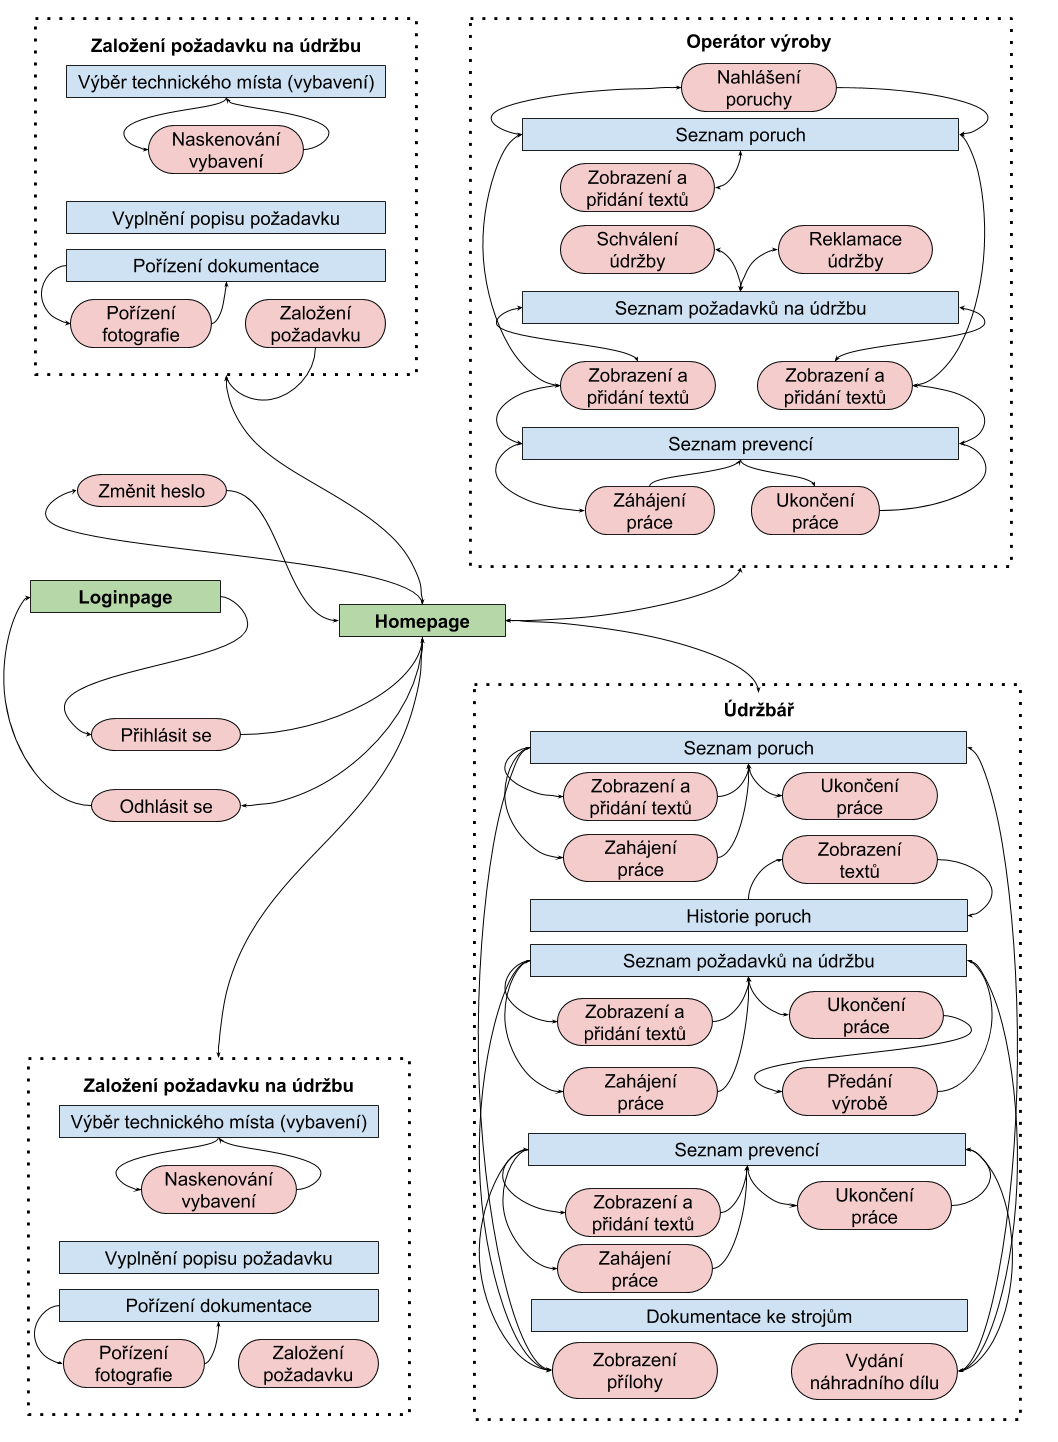
\includegraphics[width=1\textwidth]{images/task_graph.png}
	\caption{Task Graph pro aplikaci}
	\label{img:task_graph}
\end{figure}

\section{Lo-Fi prototyp}
Lo-Fi (Low-Fidelity) prototypy slouží pro snadné a hlavně rychlé znázornění pochopení konceptu a možné podoby budoucí aplikace. Demonstruje sled požadovaných procesů a informačních struktur. Díky tomu lze získat levnou zpětnou vazbu pro zlepšení aplikace. Obecně jsou charakterizovány nízkou technologickou implementací a ne zřídka k tvorbě bývá použit i obyčejný papír a tužka \cite{lofi}. 

Pro návrh prototypu byly použity dva k tomu určené nástroje. Prvním z nich je univerzální nástroj pro tvorbu prototypových aplikací Balsamiq Mockups \cite{balsamiq} druhým je nástroj Built \cite{builtme} určený k prototypování přímo ve frameworku SAPUI5. Návrh rozhraní probíhá pro dva typy zařízení. Jednak pro desktop aplikace běžně disponujícím rozlišením 1200 pixelů a více a poté i pro přenosná zařízení jako jsou chytré telefony nebo tablety. V obou případech se jedná o \textbf{WYSIWYG editory} (What You See Is What You Get), které umožňují tvořit cílovou podobu stránky bez nutnosti cokoliv programovat. Většinou pracují na principu táhni a pusť. Tudíž uživatel pracující s tímto editor si vybírá ze základny použitelných UI komponent, které potom skládá do sebe a tvoří tím výslednou stránku. 
\subsection{Balsamiq}
Jedná se o prototypovací nástroj disponující širokou škálou univerzálních kreslících nástrojů a připravených elementů, které se v moderních aplikacích vyskytují. Takovým elementem může být například obecná struktura webové stránky nebo vzhled mobilního telefonu. Tím lze vytvořit kostru navrhovaného prototypu, do kterého lze poté sázet konkrétní UI prvky jako tlačítka, texty, obrázky, tabulky a podobně. Na každý element lze navázat událost, pomocí které lze mezi jednotlivými stránkami navigovat. Výstupem je soubor ve formátu PDF, ve kterém se lze mezi jednotlivými obrazovky pohybovat jako by byly reálnou webovou stránkou nebo aplikací. 
\paragraph{Desktopová verze}
První navržená stránka se týká přihlášení uživatele. Návrh přihlašovací stránky je vidět na obrázku \ref{img:bal_login_desktop}. Byl pro ni použit layout představující webový prohlížeč. Do něj byl zasazen formulář pro vyplnění uživatelského jména a hesla. Z důvodu testování nástroje byly do stránky doplněny i doprovodné texty a náznak úvodního obrázku. 
\begin{figure}[H]
	\centering
	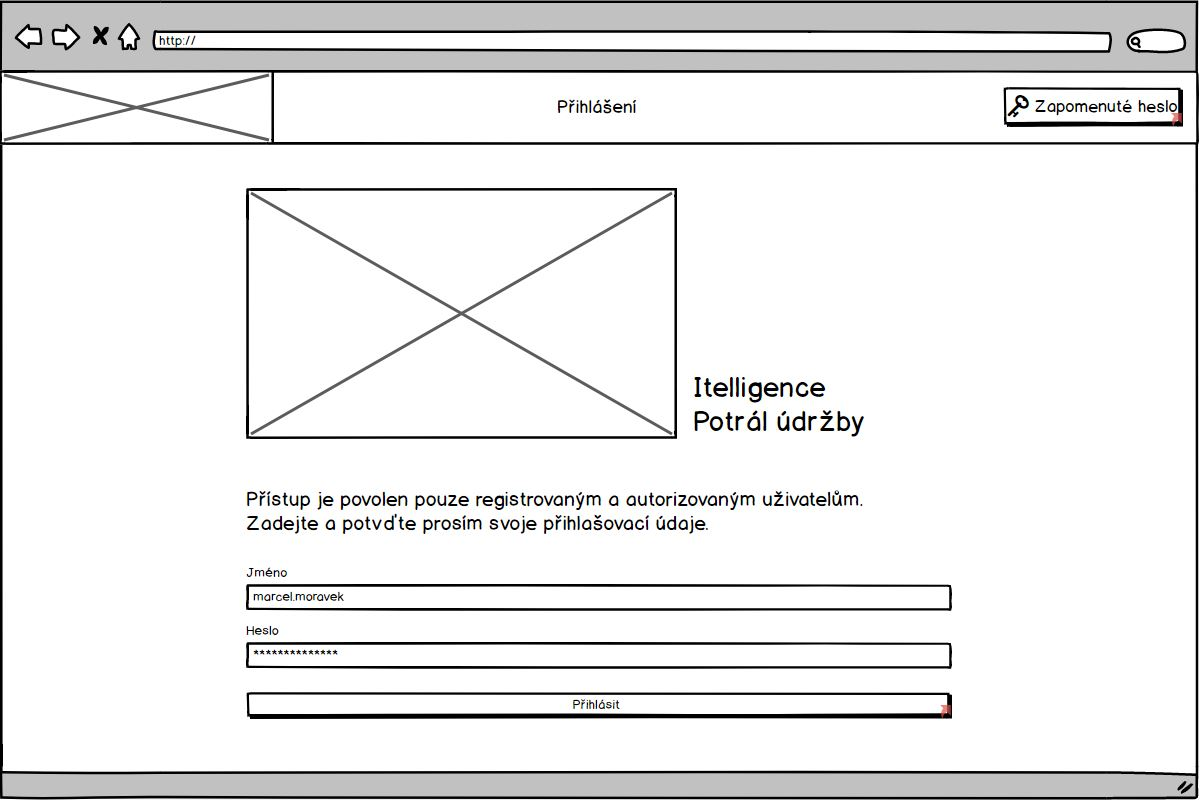
\includegraphics[width=0.9\textwidth]{images/bal_login}
	\caption{Návrh přihlašovací stránky}
	\label{img:bal_login_desktop}
\end{figure}
Pro návrh domovské stránky je čerpáno z konceptu SAP Fiori Launchpad, který slouží jako rozcestník do aplikací ve standardním licencovaném řešení SAP. Ten umožňuje uživatelům jednotlivé aplikace seskupovat a upravovat si designové téma. Ukázkou Launchpadu je obrázek \ref{img:fiori_launchpad}. 
\begin{figure}[H]
	\centering
	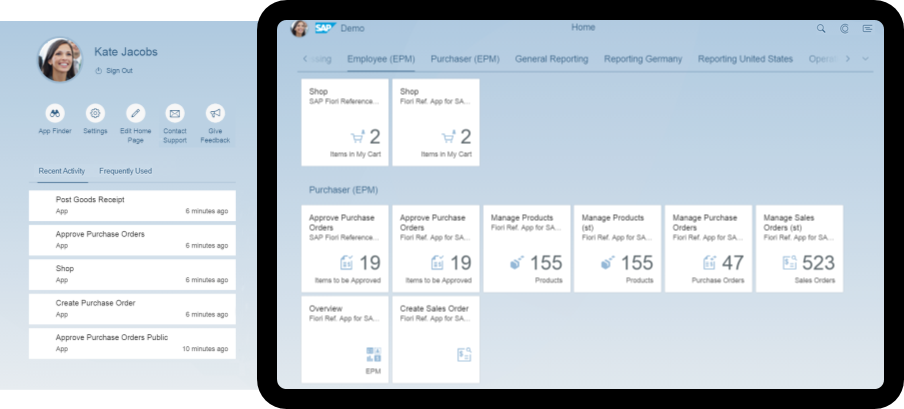
\includegraphics[width=0.9\textwidth]{images/fiori_launchpad}
	\caption{Ukázka designu SAP Fiori Launchpad}
	\label{img:fiori_launchpad}
\end{figure}
Nic takové ovšem není ve vyvíjené aplikaci plánováno. Nicméně pro důvod zachování konceptu a možného budoucího zprovoznění SAP Fiori Launchpad je přistoupeno ke stejnému dlaždicovému návrhu. Návrh je k vidění na obrázku \ref{img:bal_homepage_desktop}. Jednotlivé dlaždice umožňují navigaci do cílených aplikací navržených závěrem analýzy v kapitole \ref{sec:zav_analyzy}.
\begin{figure}[H]
	\centering
	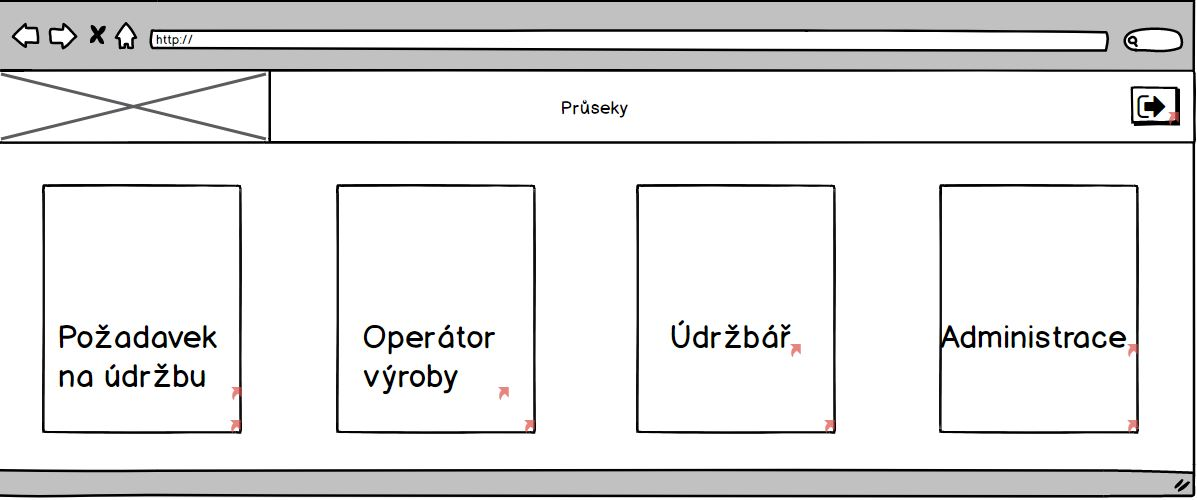
\includegraphics[width=0.9\textwidth]{images/bal_homepage}
	\caption{Návrh domovské stránky}
	\label{img:bal_homepage_desktop}
\end{figure}
Obrázek \ref{img:bal_poruchy_seznam_desktop} představuje navrženou stránku pro operátoru výroby. Skládá se z již použitého layoutu pro webové stránky a především pak tabulky zobrazující seznam poruch. V tabulce jsou zobrazeny požadované sloupce a v její pravé horní části jsou tlačítka pro přepínání druhů hlášení a spolu s tlačítkem pro založení nové poruchy. 
\begin{figure}[H]
	\centering
	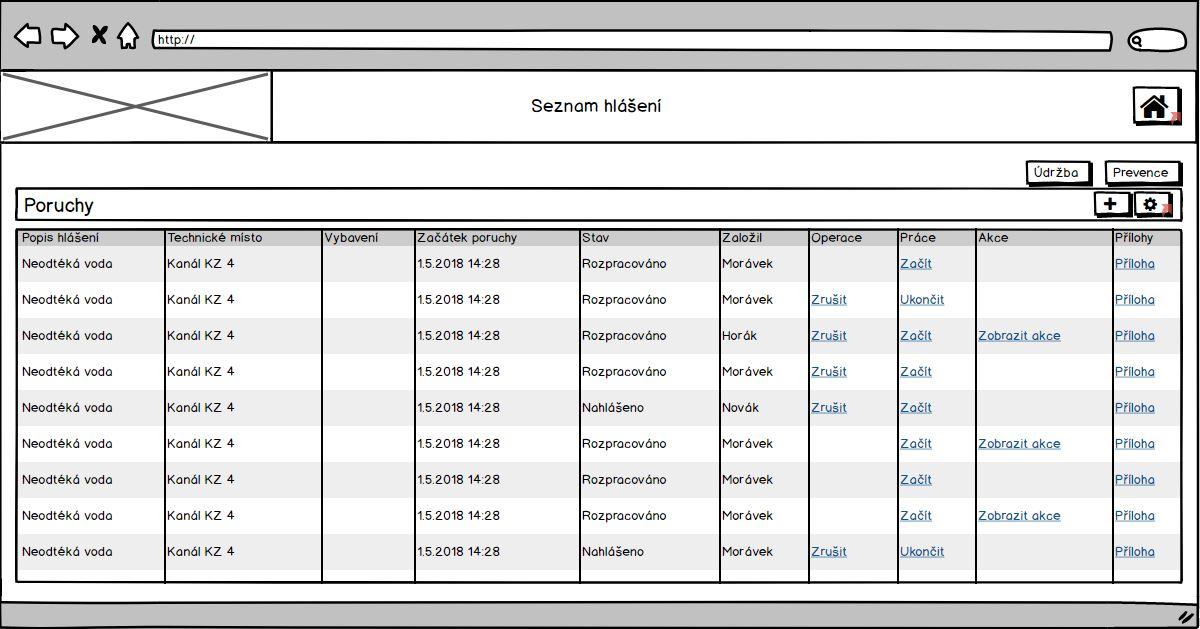
\includegraphics[width=0.9\textwidth]{images/bal_poruchy_seznam}
	\caption{Návrh seznamu poruch pro operátora výroby}
	\label{img:bal_poruchy_seznam_desktop}
\end{figure}
Po stisknutí tlačítka pro založení nové poruchy dojde k otevření dialogu, tak jak je znázorněno na obrázku \ref{img:bal_poruchy_seznam_zalozeni_poruchy_desktop}. Zobrazený dialog se zobrazí do popředí aplikace s tím, že zbytek (seznam hlášení a zbytek komponent) bude neaktivní. Formulář pro založení poruchy se skládá z několika polí, pro které jsou využity příhodné vstupní elementy. To znamená, že například pro stanovení priority je použit select box umožňující výběr z pevně dané množiny hodnot. Pro výběr souboru je naopak připraveno standardní tlačítko vyhledat, které by mělo otevřít průzkumníka pro vyhledání souboru v závislosti na uživatelovi používané platformě. 
\begin{figure}[H]
	\centering
	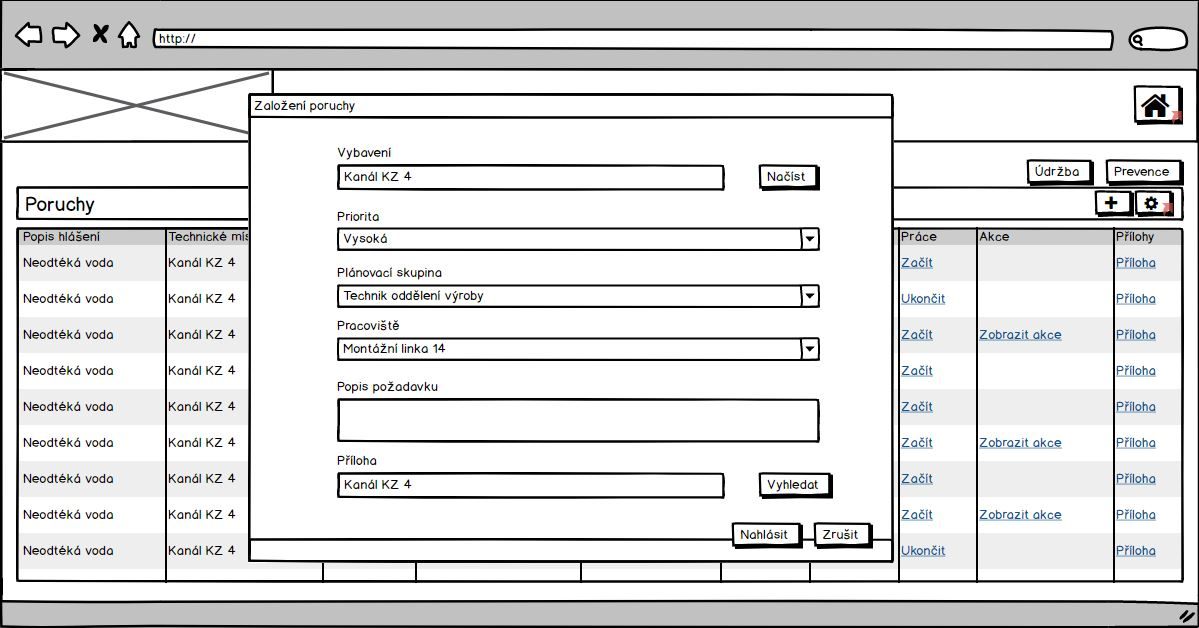
\includegraphics[width=0.9\textwidth]{images/bal_poruchy_seznam_zalozeni_poruchy}
	\caption{Návrh založení poruchy pro operátora výroby}
	\label{img:bal_poruchy_seznam_zalozeni_poruchy_desktop}
\end{figure}

\paragraph{Mobilní verze}
Mobilní verze obsahuje návrh stejných obrazovek jako desktopová verze popsaná výše. 

\begin{figure}[H]
	\centering
	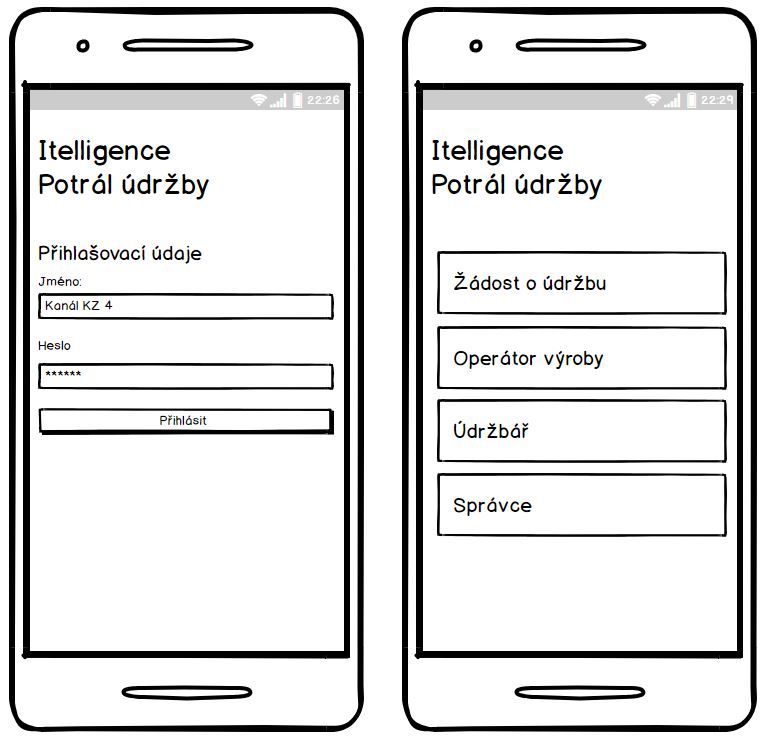
\includegraphics[width=0.8\textwidth]{images/bal_login_hompage_mob}
	\caption{Návrh přihlašovací a domovské stránky}
	\label{img:bal_login_hompage_mob}
\end{figure}

\begin{figure}[H]
	\centering
	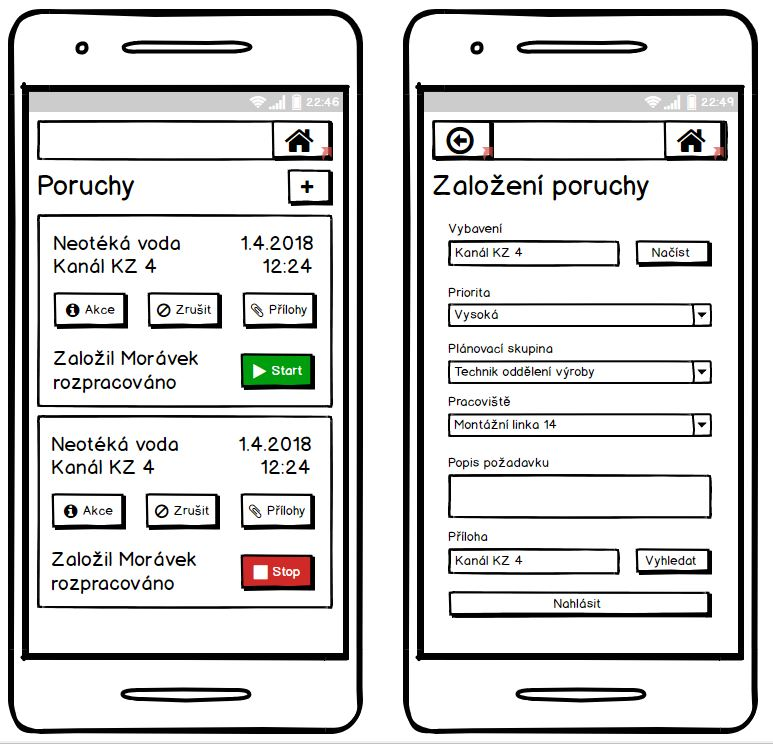
\includegraphics[width=0.8\textwidth]{images/bal_poruchy_mob}
	\caption{Návrh }
	\label{img:bal_poruchy_mob}
\end{figure}

\subsection{Built}
Jedná se o oficiální produkt společnosti SAP, který umožňuje tvorbu prototypových aplikací ve frameworku SAPUI5. Tvorba v tomto nástroji si vyžaduje alespoň základní znalosti o jednotlivých komponentách frameworku a strukturování navrhovaných stránek. Pro výběr prvků se totiž využívá omezený výběr UI komponent poskytovaných přímo frameworkem SAPUI5. V základním výběru jsou především prvky z responzivní knihovny \uv{sap.m}.
\paragraph{Desktopová verze}
První navržená stránka je pro operátora výroby. Zobrazuje mu tabulku se seznam poruch. každá porucha má ve sloupcích vypsané požadované hodnoty, případně tlačítka pro provádění požadovaných akcí. Na obrázku \ref{img:bu_poruchy_seznam} je k vidění například tlačítko pro započetí práce na poruše nebo pro zobrazené přiložené přílohy. 
\begin{figure}[H]
	\centering
	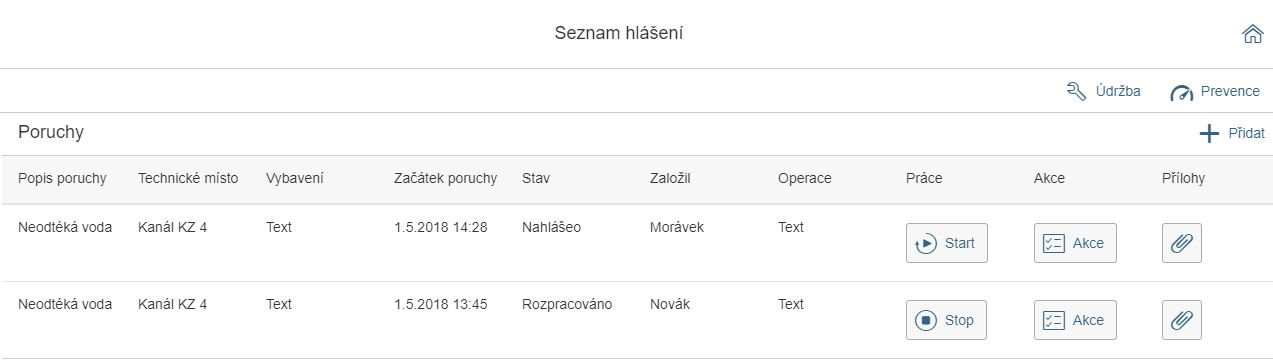
\includegraphics[width=1\textwidth]{images/bu_poruchy_seznam}
	\caption{Diagram případu užití pro správu poruch}
	\label{img:bu_poruchy_seznam}
\end{figure}
Prvním technickou překážkou tohoto nástroje je vytváření dialogů. To totiž není možné. A proto pro stlačení tlačítka na založení reakce musí dojít k zavolání zcela nové stránky. Stránka s jednotlivými elementy pro popsání poruchy a následného založení je k vidění na obrázku \ref{img:bu_zalozeni_poruchy}. 
\begin{figure}[H]
	\centering
	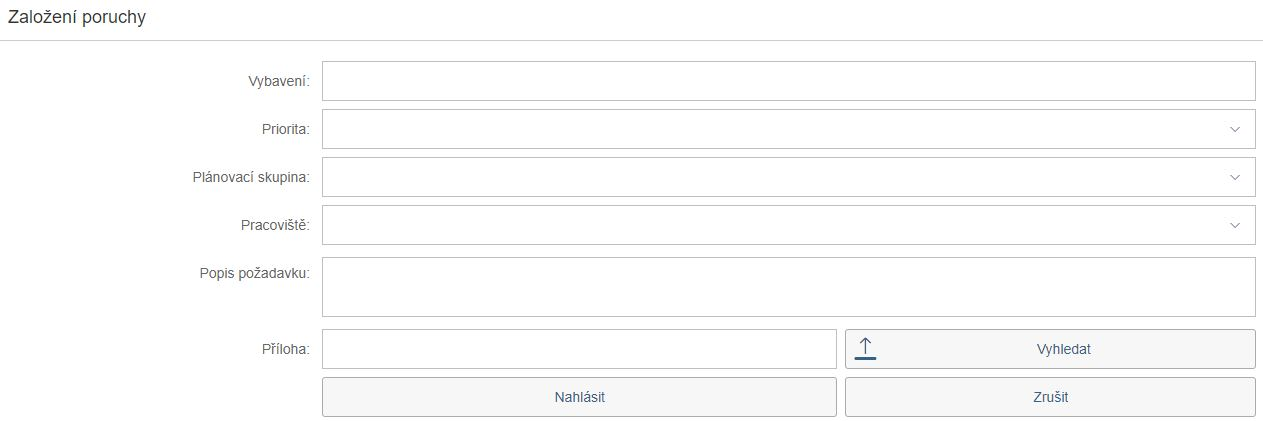
\includegraphics[width=1\textwidth]{images/bu_zalozeni_poruchy}
	\caption{Diagram případu užití pro správu poruch}
	\label{img:bu_zalozeni_poruchy}
\end{figure}

\paragraph{Mobilní verze}
Druhou technickou překážkou je tvorba návrhu pro mobilní zařízení. Knihovna \uv{sap.m} je sice responzivní, ale ne vždy nabízí takové možnosti, které by od ní mohly být očekávány. Na obrázku \ref{img:bu_mob} je k vidění podoba tabulky se seznamem poruch. Místo horizontálního skládání sloupců vedle sebe je správně použito skládání vertikální. Nicméně při zobrazení pěti hlášení by uživatel nedělal nic jiného než zdlouhavě hledal požadovanou informaci v zdánlivě nekonečném seznamu.

\begin{figure}[H]
	\centering
	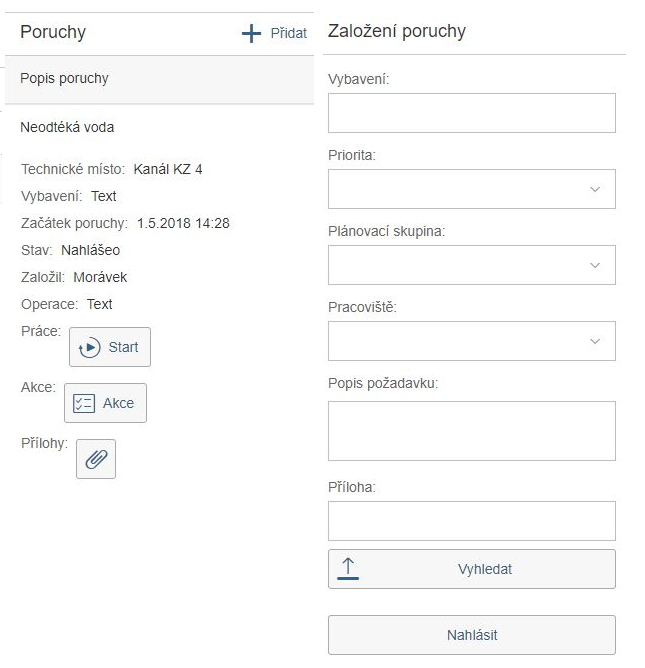
\includegraphics[width=0.8\textwidth]{images/bu_mob}
	\caption{Diagram případu užití pro správu poruch}
	\label{img:bu_mob}
\end{figure}

\subsection{Porovnání prototypovacích nástrojů}
Na porovnání použitých nástrojů je k dispozici skromná tabulka hodnocení (jako ve škole) od autora práce.
\begin{center}
	\begin{table}[H]
		\centering
		\begin{tabular}{| l | c | c |}
			\hline 
			Prostředí 						& Balsamiq 	&	Built		\\ 
			\hline	
			\hline
			Výběr komponent					&	1		&	3			\\ 
			\hline
			Rychlost prototypování			&	1		&	3			\\
			\hline
			Možnost využití při Hi-Fi		&	3		&	2			\\
			\hline
			Dostupnost (cena)				&	2		&	3			\\
			\hline		
		\end{tabular}
		\caption {Tabulka s hodnocením prototypovacích nástrojů} 
		\label{tab:prototyp_comp}
	\end{table}
\end{center}
Pro tvorbu Lo-Fi prototypu se zdáti být Balsamiq účinějším nástrojem. Je mnohem rychlejší, přehlednější a při troše úsilí a znalosti frameworku SAPUI5 lze pomocí něho dosáhnout velmi dobrých výsledků v napodobení Fiori aplikace. Nástroj Built sice navíc umožňuje následné vyexportování aplikace, nicméně 

\section{Heuristická analýza}
Při návrhu uživatelského rozhraní je dobré držet se deseti následujících pravidel z Nielsenovi heuristické analýzy. Nielsenova heuristická analýza je jednou ze základních metod pro testování uživatelského rozhraní. Jedná se o seznam pravidel, které by uživatelské rozhraní mělo splňovat. Jakob Nielsen a Rolf Molich v roce 1990 vytvořili heuristiku pro heuristické vyhodnocení a poté v roce 1994 Jakob Nielsen revidoval tuto heuristiku na množinu pravidel \cite{heursitika2}

\begin{enumerate}
	\item
	\textbf{Viditelnost stavu systému}: Uživatel by měl být vždy vhodně informován o tom co se zrovna děje. Systém by měl vždy dát uživateli vědět, co se právě odehrává. Nesmí zůstat zamrzlý a nereagovat na uživatelské vstupy.
	\item
	\textbf{Propojení systému a reálného světa}: Komunikace systému s uživatelem by se měla odehrávat uživatelsky příjemným způsobem (srozumitelný jazyk bez odborných termínů). Měl by zachovávat konvence reálného světa, ikony by měli znázorňovat akci, která se pod nimi ukrývá a podobně. 
	\item
	\textbf{Uživatelská kontrola a svoboda}: Uživatelé při práci se systémem dělají chyby a potřebují proto únikový východ pro návrat do předchozího stavu. Měla by tak být vždy k dispozici funkce zpět (návrat do předchozího stavu) nebo alespoň varování o nevratné akci. Uživatel tím pádem více experimentuje a rychleji se učí aplikaci ovládat. 
	\item
	\textbf{Standardizace a konzistence}: Uživatelé by neměli být nuceni přemýšlet, jestli různé termíny znamenají to stejné, proto se doporučuje dodržovat obecné zásady. Pokud je to možné, je vhodné používat platformové (frameworkové) komponenty pro zachování jednotného designu.
	\item
	\textbf{Prevence chyb}: Vyvarovat se chybovým hlášením bezpečným designem, který bude preventivně působit proti problémům. Uživateli je dobré například sdělit špatně vyplněný formulář ještě před tím, než se ho pokusí potvrdit a odeslat.
	\item
	\textbf{Rozpoznání namísto vzpomínání}: Uživatel by neměl být nucen vzpomínat si na provádění operací v systému, instrukce by měly být v systému vždy viditelně umístěny. Musí tak být vždy zobrazeny relevantní údaje pro uživatelovu práci. 
	\item
	\textbf{Flexibilní a efektivní použití}: Umožnění zrychlení práce se systém pro pokročilé uživatele. Mělo by tak být umožněno pokročilým uživatelům zpřístupnit pokročilý režim, zobrazující například méně informaci nebo s méně kroky v procesu.
	\item
	\textbf{Estetický a minimalistický}: Uživatel by měl mít co nejméně možností kam může kliknout, protože každá další možnost soutěží o pozornost uživatele. Čím méně možností uživatel má,	tím rychleji je schopen pokračovat. Na obrazovce by také měly být zobrazeny pouze informace, které uživatel v dané situaci opravdu potřebuje.
	\item
	\textbf{Pomoc uživatelů pochopit, poznat a vzpamatovat se z chyb}: Chybové hlášky by měly být v přirozeném jazyce a neměly by například obsahovat žádné chybové kódy a podobně. Nejlepší je ovšem nedojít do stavu, kdy je chybového hlášení třeba.
	\item
	\textbf{Nápověda a návody}: Všechny informace se musí dát lehce vyhledat, nápověda by měla obsahovat postupy. Spíše než popisy by se měla zabývat příklady.
\end{enumerate} 

\textbf{Jedná se o pomůcky poskytovanou testerům UI, nicméně se jedná o velmi užitečné zásady už pro samotný návrh.}

% % % % % % % % % % % % % % % % % % % % % % % % % % % % % % % % % % % % % % % % % % % % % % % % % % % % % % % % % % % % 


\chapter{Implementace}
\label{chap:implementace}
Tato kapitola se věnuje implementaci jednotlivých částí navržené architektury, která je ihned v první podkapitole zobrazena a popsána. Podrobnější popis jednotlivých komponent následuji ihned poté. 

\section{Architektura}
Architektura celého systému je zobrazena na obrázku \ref{img:architektura}, je rozdělena do tří bloků a tomu odpovídají i tři následující podkapitoly. 

Standardním řešením je Fiori aplikace nahraná v SAP GW, která je přístupná přes SAP Fiori Launchpad. Pokud však zákazník nedisponuje dostatečnými licencemi a zakoupenými moduly, není tato cesta možná. Proto je zde navrženo řešení, které Fiori aplikaci spouští v prostředí Apache Tomcat a komunikaci s prostředím SAP řeší pomocí Java servletů a SAP BSP. 

Toto řešení ovšem při požadavcích jako autentizace a autorizace uživatele přináší vývoj navíc. Ten však nemusí a zpravidla nepřesahuje náklady na moduly a licence SAP. Naopak přináší řadu výhod. V prostředí Apache Tomcat lze uchovávat a zpracovávat přijatá data a vytvořit si tak komunikační mezivrstvu mezi Fiori aplikací a SAP ERP. Tím lze ulehčit potenciálně zatíženým serverům a zkrátit uživateli webové aplikace odezvu v komunikaci.

\begin{figure}[H]
	\centering
	\includegraphics[width=1\textwidth]{images/architektura}
	\caption{Architektura navrženého systému}
	\label{img:architektura}
\end{figure}

\section{SAP ERP}
Touto části architektury se tato práce přímo nezabývá, nicméně je zde pro lepší představu o celkovém systému krátce popsána. Jak již bylo v kapitole \ref{sec:erp} věnující se teoretickému základu řečeno, místem veškerých potřebných procesů pro realizaci požadované aplikace je SAP ERP. Konkrétně potom moduly PM, MM a CO. Každý z těchto modulů má desítky BAPI (Business Application Programming Interface) funkcí představujících rozhraní pro základní operace nad daným modulem. Správné sekvence a data volaných BAPI funkcí jsou potom obaleny do funkčních modulů, které umožňují vzdálené volání z jiných systémů. K tomu slouží v rámci SAP funkcionalita RFC (Remote Function Call), které umožňuje přenášet data napříč jednotlivými systémy. Takovýchto funkcí vzniklo v ERP systému více než 20, výčet modulů je k vidění na obrázku \ref{img:erp_fm}.

\begin{figure}[H]
	\centering
	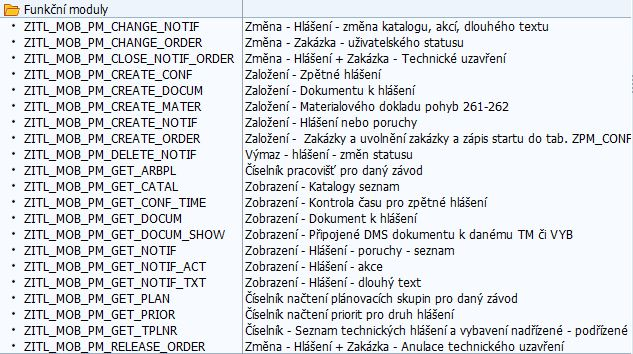
\includegraphics[width=1\textwidth]{images/erp_fm}
	\caption{Seznam funkčních modulů v ERP systému}
	\label{img:erp_fm}
\end{figure}

\section{SAP GW}
Primárním účelem serveru SAP GW (Gateway) je komunikace s okolním světem. Je také standardním prostředím pro běh Fiori aplikace a pro servisy pomocí protokolu OData popsaných v kapitole \ref{ssec:odata}. Ne všichni zákazníci ovšem mají nakoupené licence pro provoz Fiori touto cestou, a právě proto byla navržena tato architektura založená na technologii BSP, která je běžně dostupná v produktech GW, ale i ERP. Na obrázku \ref{img:gw_json} je seznam 36 BSP stránek, které pro aplikaci vznikly. V porovnání s počtem funkčních modulů na straně ERP je evidentní, že nejsou vytvořeny v poměru 1:1. Je to především z toho důvodu, že jsou v této úrovni uloženy uživatelská data portálových uživatelů. 

\begin{figure}[H]
	\centering
	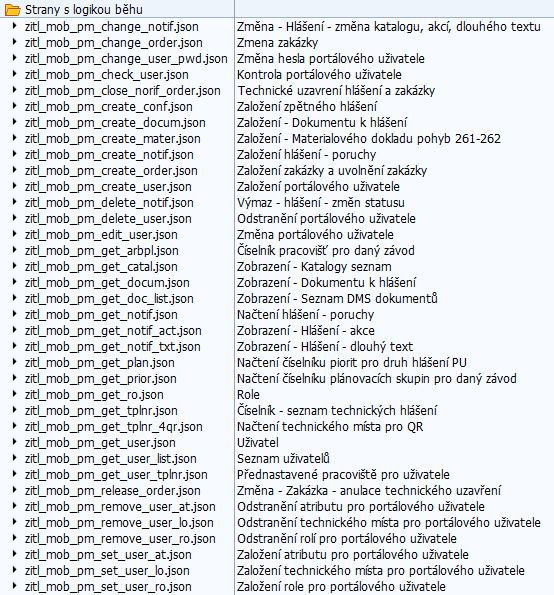
\includegraphics[width=1\textwidth]{images/gw_json}
	\caption{Seznam funkčních modulů v SAP GW}
	\label{img:gw_json}
\end{figure}

Všechny výše zobrazené BSP stránky jsou implementovány na stejném principu. Využívají události OnRequest, ve které dojde ke zpracování vstupních dat a vygenerování adekvátních dat na výstup. V první fázi jsou vytvořeny lokální proměnné potřebné pro správné zpracování dat. Následně je deserializován vstupní objekt typu JSON do odpovídajících struktur programovacího jazyka ABAP. Poté je pomocí RFC zavolán příslušný funkční modul. Stejně tak jako v ukázce algoritmu \ref{code:rfc_call}. 

\begin{algorithm}[H]	
	\begin{lstlisting}[language = VHDL]  
CALL FUNCTION 'ZITL_PM_CREATE_NOTIF' DESTINATION lv_dest
  EXPORTING
    is_notif_get = zitl_input_json-qmart
    it_tplnr     = zitl_input_json-tplnr
  IMPORTING
    et_notif     = lt_notif
    ev_error     = lv_error.
	\end{lstlisting}
	\caption{RFC volání funkčního modulu}	
	\label{code:rfc_call}
	\small Kód zobrazuje volání funkčního modulu ZITL\_MOB\_PM\_GET\_NOTIF pro načtení seznamu hlášení. Parametrem DESTINATION je řízeno směrování volání. Hodnotou musí být nastavené spojení se vzdáleným serverem zabezpečeného pomocí metody BASIC. Parametry EXPORTING a IMPORTING určují vstupní a výstupní proměnné z funkčního modulu. Vstupními parametry je tak řízen například typ hlášení, který určuje, zdali se jedná o poruchu, prevenci nebo požadovanou údržbu. Obsahuje však i další parametry určují datumový rozsah a podobně.
\end{algorithm}	

Načtená data jsou zpětně serializována pro výstup. Obsahem celé BSP HTML stránky je tedy objekt typu JSON. Jak již ale bylo zmíněno, na úrovni GW se nacházejí i uživatelská data představující portálové uživatele. Na následujícím obrázku \ref{img:gw_db} je k vidění ilustrační databázové schéma. 

\begin{figure}[H]
	\centering
	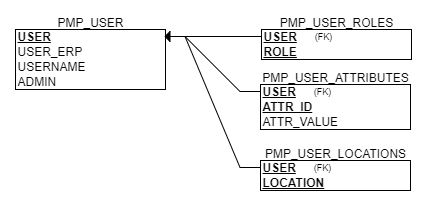
\includegraphics[]{images/gw_db}
	\caption{Ilustrační databázové schéma pro uživatelská data portálového uživatele}
	\label{img:gw_db}
\end{figure}

Databázové schéma neodpovídá úplně přesně skutečnosti. Některá pole a vazby tabulek jsou úmyslně skryta, a to buď protože nejsou pro celý koncept aplikace relevantní nebo z důvodu zvýšení bezpečnosti. Ze schématu vychází vazby 1 ku N pro všechny kombinace kmenové tabulky PMP\_USER a pomocných tabulek PMP\_USER\_ROLES, PMP\_USER\_ATTRUBUTES a PMP\_USER\_LOCATIONS. Trochu podrobněji jsou jednotlivé tabulky popsány v následujícím výčtu.

\begin{itemize}
	\item
	\textbf{PMP\_USER}: Tabulka obsahuje záznamy jednotlivých portálových uživatelů. Jedná se tedy především o přihlašovací údaje a jednotlivé informace přímo související s uživatelem. Jako je například jméno, pod kterým uživatel ve webové aplikaci vystupuje, osobní číslo v ERP, informace o tom, zdali se jedná o správce nebo také platnosti uživatele a data s časy posledních změn spolu s jejich autory.
	\item
	\textbf{PMP\_USER\_ROLES}: Tabulka s cizím klíčem uživatel. Primární klíč je identifikátor role, která je uložena ve standartních SAP tabulkách, které jsou zpracovatelné pomocí standardních transakcí.
	\item
	\textbf{PMP\_USER\_ATTRIBUTES}: Tabulka s cizím klíčem uživatele. Primární klíč je identifikátor atributu. Výčet atributů není nikterak stanoven a zodpovědnost za správné vyplnění je přenesena na správce účtů, který má k dispozici seznam užitečných atributů pro webovou aplikaci. Součástí tabulky je i pole pro hodnotu takového atributu. S vytvořením aplikační logiky kontrolující správnost atributů z pevně stanového výčtu je počítáno v budoucím rozšíření aplikace.
	\item
	\textbf{PMP\_USER\_LOCATIONS}: Tabulka s cizím klíčem uživatele. Primární klíč je identifikátor zodpovědného pracoviště. Ten není prozatím nikterak kontrolován vůči hierarchickému uspořádání technických míst v modulu SAP PM. S vytvořením aplikační logiky kontrolující správnost pracovišť ze stanovené hierarchie je počítáno v budoucím rozšíření aplikace.
\end{itemize} 

\section{Apache Tomcat}
Apache Tomcat je známý open-source webový server a servletový kontejner. Jedná se o oficiální referenční implementaci technologií Java Servlet a Java Server Pages (JSP). Na serveru mohou běžet uživatelské servlety (programy napsané v Javě), které umí zpracovávat požadavky zasílané pomocí HTTP protokolu a tímtéž protokolem na ně odpovídat. Apache Tomcat zde slouží jako zásobník servletů starající se o jejich spouštění, běh, ukončování a podobně \cite{tomcat}.

\subsection{Login Modul}
\label{ssec:login_modul}
Login modul využívá systému \textbf{JAAS} (Java Authentication and Authorization Service), který slouží pro autentizaci a autorizaci uživatele. Jak již z názvu vyplývá, jedná se o bezpečnostní systém založený na technologii Java. Vyskytuje se od verze 1.4 v J2EE (Java 2 Enterprise Edition). Veškeré informace týkající se JAAS technologie vycházejí z dokumentace \cite{jaas}

Deklarativní zabezpečení J2EE chrání webové aplikace podle aktuálního vzorce uživatelovi URL. Cesta k souborům může být popsána absolutním i relativním způsobem. Jeli například požadováno povolení přístupu k aplikaci uživatelům s rolí USERS, je zapotřebí v definici web.xml \ref{item:pm_web_inf} zavést následující definici.

\begin{algorithm}[H]	
	\begin{lstlisting}[language = XML]  
<security-constraint> 
  <web-resource-collection> 
    <web-resource-name>AllPublic</web-resource-name> 
    <url-pattern>/</url-pattern> 
  </web-resource-collection> 
  <auth-constraint> 
    <role-name>USERS</role-name> 
  </auth-constraint> 
</security-constraint>
	\end{lstlisting}
	\caption{Definice zabezpečení aplikace pro roli USERS}	
	\label{code:j2ee_definition}
	\small Tato definice chrání webovou aplikaci od kořenového adresáře J2EE, jak je naznačeno vzorem \uv{\textbackslash}. Pokud by mělo být zabezpečení aplikováno jen na část aplikace, je třeba uvést za \uv{\textbackslash} jméno adekvátního podadresáře.
\end{algorithm}	

Ověřování v deklarativní ochraně je vynuceno, právě tehdy když si uživatel vyžádá chráněnou oblast webové aplikace. Pokud nebyl dříve ověřen, zobrazí se přihlašovací dialog, aby se uživatel mohl identifikovat. Běžně používané způsoby ověření jsou FORM a BASIC. 

\paragraph{BASIC} Je základním typem autentizace. Využívá standardního dialogu prohlížeče pro vložené uživatelského jména a hesla. Tento dialog nelze nikterak modifikovat, proto se jeho vzhled liší pouze na typu aktuálně používaného prohlížeče. Uživatelská pověření pro autentizovanou oblast jsou uložena v rámci session prohlížeče. Uživatelská data (jméno a heslo) jsou potom v zakódované formě posílána s každým HTTP requestem \cite{basic_form}.

\begin{algorithm}[H]	
	\begin{lstlisting}[language = XML]  
<login-config> 
  <auth-method>BASIC</auth-method> 
</login-config>
	\end{lstlisting}
	\caption{Definice typu autentizace BASIC}	
	\label{code:auth_basic_def}
\end{algorithm}	

\paragraph{FORM} Je přizpůsobivější variantou autentizace. Umožňuje vývojáři specifikovat vlastní dialog pro přihlášení. Jediné omezení spočívá v pojmenování vstupní hodnoty uživatelského jména na j\_username a hesla na j\_password. Přihlašovací akce pro autentizaci potom musí mít hodnotu j\_security\_check v rámci J2EE kontejneru. Uživatel posléze zůstává ověřen přes session server \cite{basic_form}.

\begin{algorithm}[H]	
	\begin{lstlisting}[language = XML]  
<login-config> 
  <auth-method> FORM</auth-method> 
  <form-login-config> 
    <form-login-page>/login.html</form-login-page>
    <form-error-page>/login_error.html</form-error-page>
  </form-login-config> 
</login-config>
	\end{lstlisting}
	\caption{Definice typu autentizace FORM}	
	\label{code:auth_form_def}
	\small Navíc od autentizace typu BASIC jsou zde zadefinovány dvě html stránky. Element <form-login-page> stanovuje stránku, která je uživateli zobrazena při prvotním pokusu uživatele o načtení aplikace, stránka stanovená elementem <form-error-page> se zobrazí v případě, že uživatel zadá špatnou kombinace jména a hesla nebo se v průběhu autentizace vyskytne jiná chyba.
\end{algorithm}	

Oba přístupy autentizace jsou zranitelná vůči útokům skrze odposlouchávání. Proto je silně doporučeno zpřístupňovat aplikaci skrze HTTPS protokol. 

Kompletní proces autentizace a autorizace je implementován pomocí tříd napsaných v programovacím jazyce Java. Výčet tříd odpovídá struktuře \ref{img:loginmodule_structure} zobrazené níže. 

\begin{figure}[H]
	\centering
	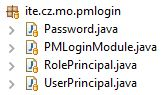
\includegraphics[]{images/loginmodule_structure}
	\caption{Struktura paketu realizující autentizaci a autorizaci}
	\label{img:loginmodule_structure}
\end{figure}

Nejdůležitější třídou je \textbf{PMLoginModule}, která spočívá v přepisu čtyř procesních metod. Inicializační metodou je \textbf{initialize}, která nastavení instančním proměnným výchozí hodnoty. Prvním z nich je základní objekt CallbackHandler, sloužící k předávání hodnot mezi modulem a uživatelovým prohlížečem. Druhým je objekt Subject udržující informace o uživateli. Takovou hodnotou je například identifikátor session. Metodou realizující autentizaci je metoda \texttt{\textbf{Login}}, která pomocí objektu CallbackHandler získá uživatelem vyplněné hodnoty jména a hesla, jejíž ověření se právě v rámci této metody musí provést. Pro kontrolu očekávaného slouží statická třída \textbf{Password}, která obsahuje metody pro generování hesel i ověření jejich shodnosti. Výstupem je potom boolean hodnota true nebo false. O autorizaci se stará metoda \texttt{\textbf{Commit}}, jejíž úkolem je přidělení příslušných rolí uživateli. K tomu slouží třídy \texttt{\textbf{UserPrincipal}} a \textbf{RolePrincipal} reprezentující jednotlivé role a uživatele. Poslední metodou k doplnění celého procesu je \textbf{Logout}, která má za úkol odstranit uživateli role a následně celý objekt Subjekt, který ho reprezentuje.

\paragraph{Nasazení} Celý projekt je zapotřebí zabalit do archivu typu JAR, sloužící pro distribuci programů a knihoven. Následně ho vložit do run-time prostředí Tomcat serveru. Pro uložení takové knihovny je určen adresář libs.

K tomu, aby server vůbec věděl, že má pro aplikace vyžadující autentizaci uživatele použít vytvořenou JAR knihovnu, je zapotřebí definovat JAAS konfigurační soubor obsahující cestu k dané knihovně. Ukázka takové definici je v kódu \ref{code:jaas_config}. 

\begin{algorithm}[H]	
	\begin{lstlisting}[language = VHDL]  
pmloginmodule {
  ite.cz.mo.pmlogin.PMLoginModule required debug=true;
};
	\end{lstlisting}
	\caption{Konfigurační soubor JAAS}	
	\label{code:jaas_config}
\end{algorithm}	

Cestu souboru je pak zapotřebí definovat v Java parametrech serveru. K určení konfiguračního souboru slouží parametr Djava.security.auth.login.config. Hodnotou k tomuto parametru je absolutní cesta požadovaného souboru.

\subsection{GW Servlet}
Na obrázku \ref{img:gw_servlet_structure} je k vidění struktura paketu realizujícího mezivrstvu pro komunikace s SAP GW. 
\begin{figure}[H]
	\centering
	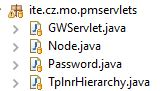
\includegraphics[]{images/gw_servlet_structure}
	\caption{Struktura paketu realizujícího middleware vrstvu mezi PM SAPUI5 aplikací a SAP GW}
	\label{img:gw_servlet_structure}
\end{figure}
Jedná se o čtyři třídy napsané v programovacím jazyce Java. Podrobněji jsou jednotlivé třídy popsány v seznamu níže.

\begin{itemize}
	\item
	\textbf{GWServlet}: Je Java třída implementující interface javax.servlet.Servlet sloužící pro zpracování Http požadavků. Základem tohoto servletu je přepsaná metoda doGet, která obsahuje parametry HttpServletRequest a HttpServletResponse umožňují jednak načtení přijatých dat společně s dalšími parametry, které s sebou požadavek nese a potom také adekvátní data pomocí odpovědi vrátit. Metoda doGet je volána z další přepsané metody doPost, která je vyvolána v případě HTTP requestu typu POST. 
	\item
	\textbf{Node}: Třída reprezentující prvek hierarchie technických míst a vybavení z modulu SAP PM. Jelikož se v interně technické místo a vybavení datově liší, je vytvořena tato třída, která nesrovnalosti mezi těmito objekty eliminuje. Datově rozdílné identifikátory jsou nahrazeny jednotným id a ostatní lišící se parametry jsou sloučeny do atributů třídy odpovídajícím významu původního datového objektu. To posléze umožňuje v prezentační vrstvě lehce pracovat v 
	\item
	\textbf{TplnrHierarchy}: Třída sloužící pro hierarchické skládání. Jejím hlavním atributem je množina (Set) objektů TplnrHierarchy. Tím, že lze uložit stejné prvky do sebe lze vytvořit požadovaná stromová struktura. Při pozdějším načítání struktury od požadovaného místa stačí v logaritmickém čase najít požadovaný uzel a vzít všechny jeho následníky.
	\item
	\textbf{Password}: Statická třída obsahující statické třídy pro generování hash z hesel a opačně k i jejich kontrolování.
\end{itemize} 

\section{PM SAPUI5 Aplikace}
V následujících podkapitolách je popsána implementační struktura projektu pro PM SAPUI5 Aplikaci. Jelikož se jedná o stěžejní část celkové architektury, obsahuje veškerou logiku očekávanou od prezentační vrstvy. Jsou zde nadefinovány veškeré pohledy (stránky), se kterými se uživatel bude moci setkat.  

\subsection{Struktura aplikace}
\label{ssec:struckuta_pm_aplikace}
Zde zobrazena a popsána celková struktura aplikace z vývojářského pohledu. Na obrázku \ref{img:pmfiori_app_struct} je k vidění hlavní strom adresářů a souborů v použitém Eclipse projektu. 

\begin{figure}[H]
	\centering
	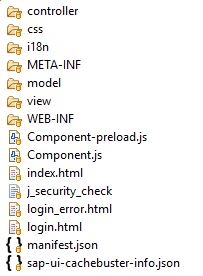
\includegraphics[]{images/fiori_app_struct}
	\caption{Struktura PM aplikace s hlavní prezentační logikou}
	\label{img:pmfiori_app_struct}
\end{figure}

Jednotlivé položky jsou potom popsány v následujícím seznamu. Koncepčně je popis strukturován tak, že nejdříve jsou napsány obecné vlastnosti očekávané od daného adresáře nebo souboru a poté jsou dopsány případné poznámky z implementace.

\begin{itemize}
	\item
	\textbf{WEB-INF}: \label{item:pm_web_inf} Adresář obsahuje externí knihovny potřebné pro správnou funkčnost aplikace. Jelikož základní datovou reprezentací používanou v této aplikaci je JSON a programovací jazyk Java nativně práci s tímto formátem nepodporuje, je v tomto adresáři přiložena externí knihovna \textbf{java-json.jar}, která práci s tímto typem objektů umožňuje. Dále je zde uložen soubor \textbf{web.xml} popisující nasazení webové aplikace včetně jejich webových služeb. Slouží k deklaraci servletů a filtrů používaných danou webovou službou. V případě této aplikace se jedná například o GWServlet.
	\item
	\textbf{view}: Složka obsahuje zadefinovaná view (UI rozvržení elementů) ve značkovacím jazyce XML. Hlavním úkolem těchto souborů je hierarchické rozvržení použitých komponent jednotlivých stránek. Pomocí různých layoutů tak umožňuje jasně definovat, že dané view reprezentuje dialog, jehož obsahem je formulář o pěti prvcích, z nichž každý používá jinou vstupní uživatelskou komponentu. Podrobněji se jednotlivým souborům věnuje podkapitola views. 
	\item
	\textbf{controller}: Adresář obsahující controllery napsané v programovacím jazyce JavaScript. Slouží především pro obsloužení uživatelské interakce s aplikací. Klikne-li například uživatel na tlačítko přidat uživatele, právě zde se nachází část kódu, která požadovanou funkcionalitu provede. Dojde například k přípravě dat pro dialog obsahující potřebná pole pro založení nového uživatele. Jednotlivým souborům se podrobněji věnuje kapitola controllery níže.
	\item
	\textbf{css}: Obsahuje soubory pro úpravu kaskádových stylů. Jelikož aplikace využívá z drtivé většiny pouze předdefinované styly frameworku SAPUI5, je zde pouze jeden soubor style.css obsahující pár úprav oproti standardu.
	\item
	\textbf{i18n}: Pro internacionalizaci se používá numeronymum i18n a v tomto případě adresář obsahuje soubory s dvojicemi hodnot klíč - hodnota, které slouží pro zobrazení v textu požadovaného jazyku. K rozlišení jazyků se používá postfix v názvu souborů. Pro český jazyk je to například název i18n\_cs.properties, určený dle koncovky \_cs. Seznam koncovek odpovídá \textbf{standardu ISO 639-2}.	
	\item
	\textbf{model}: Obsahuje pomocné JavaScriptové soubory s funkcemi, které se opakovaně používají napříč celou aplikací. Jedná se například o formátovací funkce, stanovení modelů obsahující informace o používaném zařízení uživatele a podobně. V mém případě obsahuje tři následující soubory.
	\begin{itemize}
		\item
		\textbf{models.js}: Slouží pouze k zadefinování modelu s informace o používaném zařízení. Poskytuje tak napříč zbytku aplikace například aktuální šířku displeje, používaný operační systém nebo typ prohlížeče. Na základě toho poté dochází ve zbytku aplikace k používání komponent příslušných dané velikosti displeje, nedochází tak k zobrazování tabulky na mobilním zařízení, ale k adekvátně upravenému listu záznamů.
		\item
		\textbf{formatter.js}: Obsahuje funkce pro úpravu zobrazované informace získaných z backendu. SAPí interní formát data 2018-05-04, lze tak pomocí takových funkcí převést na datum v požadovaném tvaru a naopak.
		\item
		\textbf{utils.js}: \label{file:utils.js} Disponuje především funkcemi pro určení, zdali se má daná komponenta zobrazovat. Například tlačítko pro schválení údržby u operátora výroby musí být zobrazené pouze v případě, že na něm údržbáři dokončili práce. Na základě statusu hlášení poté funkce vrací boolean hodnoty true nebo false pro zobrazení daného tlačítka. Dále jsou zde funkce pro přeposílání dat na GWServlet využívající AJAX, který umožňuje asynchronní komunikaci pro výměnu dat s backendem. 
		\begin{algorithm}[H]
			\begin{lstlisting}[language=java]      
query : function(data, success, error) {
  $.ajax({
    type : 'POST',
    url : url,
    cache : false,
    async : true,
    data : data,
    dataTye : "json",
    success : success,
    error : error
  });
},
			\end{lstlisting}
			\caption{Ukázka AJAX volání}	
			\label{code:ajax}
			\small Tato funkce se používá u každého volání z aplikace na GWServlet pro následné zpracování na backendu. Na vstupu jsou tři parametry. Data obsahuje serializovaný JSON objekt obsahující potřebná data. Parametry success a error jsou ukazateli na funkce, které se mají vykonat v případě (ne)úspěšného volání AJAXu. 
		\end{algorithm}	
		
		
	\end{itemize} 
\end{itemize} 

\begin{itemize}
	\item
	\textbf{Component.js}: Jeden ze stavebních kamenů celé aplikace. Představuje objekt obalující všechna zadefinovaná view. Tudíž jakékoliv informace uložené v modelu jsou dostupné napříč celou aplikací. Právě zde se uplatní modely nesoucí znalosti o použitém zařízení klienta nebo sloužící pro překlady textů.
	\item
	\textbf{index.html}: Jedná se o soubor, který je implicitně volán v případě, že uživatel ve svém webovém prohlížeči zadá adresu, pod kterou se požadovaná aplikace skrývá. Nacházejí se zde základní informace nutné pro správné spuštění aplikace. Nejdůležitější z nich je zadefinování zdrojů frameworku SAPUI5. To spočívá v odkazu na obsáhlý soubor sap-ui-core.js (dále již jen jádro), které představuje kostru nutnou pro běh aplikace. Použití slova core - jádro v názvu pochopitelně není náhoda. Jádro si v průběhu používání aplikace dotahuje další frameworkové knihovny jako jsou například komponenty pro uživatelské vstupní pole typu datum, kdy je uživateli poskytnuto příjemné kalendářní rozhraní pro výběr požadovaného data. Tyto knihovny jsou stahovány až v případě, že si je uživatelova interakce vyžaduje. Dochází tedy k tak zvanému lazy loadingu. Stanovit přístup k jádru se dá pomocí dvou základních metod. První z nich je mapování na veřejně dostupný soubor pod adresou \url{https://sapui5.hana.ondemand.com/resources/sap-ui-core.js}. Druhým způsobem je mít veškeré knihovny dostupné v run-timeovém prostředí aplikace. Zároveň se také jedná o možnost použitou v této implementaci. Interní bezpečností politika totiž nedovoluje volání mimo vnitřní síť. Dále se zde nacházejí odkazy na externí knihovny nutné pro správný chod aplikace v rámci prostředí používaném uživatelem. V rámci hierarchie HTML je vytvořen element body, do kterého je vložena celá instance vytvořené aplikace odvozené od staženého jádra. Jedná se zpravidla o jediný kus čistého HTML při tvorbě aplikace ve frameworku SAPUI5.
	\paragraph{Aplikační Cache} Implicitně jsou veškeré zdroje a knihovny používané ve frameworku ukládány do mezipaměti prohlížeče, aby byla uživateli zkrácena doba načítání a nedocházelo k opakovanému stahování potřebných souborů. To s sebou ovšem přináší problém při vydávání nové verze aplikace. V případě, že by došlo ke změně některého ze souborů a libovolný uživatel měl uloženy staré soubory v mezipaměti, pravděpodobně by se stala aplikace nefunkční. Tento problém je oficiálně řešen na straně SAP Gateway, kde dochází k porovnání jednotlivých soborů před samotným stažením. Tato funkcionalita bohužel není implicitně ve frameworku zanesena, nicméně existují mechanismy, které obdobné chování umožňují. Celý proces spočívá v zadefinování ResourceServletu, který porovnává datum poslední modifikace souboru s tím, který má uživatel uložen v mezipaměti. Tento Servlet musí být zadefinován v souboru web.xml a aplikace musí dostat informaci o tom, u kterých souborů má k takové kontrole docházet. Proto je v tomto HTML souboru odkaz na soubor \textbf{sap-ui-cachebuster-info.json}, obsahující JSON pole, s dvěma prvky. Jedním z nich je relativní cesta k požadovanému souboru a druhým je datum poslední modifikaci. Pro správný chod aplikace je tak nutné při každém exportování dbát na aktualizaci potřebných záznamů.
	\item
	\textbf{login.html}: V rámci JAAS logiky pro autorizaci a autentifikaci je definována implicitní HTML stránka, která je vyvolána v případě, že uživatel nemá doposud vytvořenou vůči aplikaci session. Z důvodu zachování konzistetního vzhledu aplikací je i pro přihlášení vytvořena SAPUI5 aplikace. Umístit ji zde v rámci jednoho projektu by způsobilo značnou nepřehlednost a taktéž by mohlo způsobit neočekáváné problémy při vývoji. Z toho důvodu má HTML stránka login.html velmi jednoduchou funkčnost. A tou je přesměrování uživatele do přihlašovací SAPUI5 aplikace.
	\item
	\textbf{manifest.json}: Manifest slouží především k rychlému definování možného směrování v rámci aplikace. Dochází zde k mapování uživatelovi aktuální url na jednotlivá view. Lze tak například přiřadit k postfixu pm/\#/vyroba view \uv{Vyroba} a tím tak uživateli zobrazit očekávané informace. Dále se zde dají zadefinovat modely přiřazené komponentě nebo zdroje kaskádových stylů. 
\end{itemize} 

\subsection{Jednotlivé stránky aplikace}
V této kapitole jsou popsány a zobrazeny nejdůležitější stránky aplikace. Koncept popisování jednotlivých stránek je velmi podobný. Nejdříve je obecně popsáno, co vlastně daná stránka dělá, poté následují dvě trochu více technické sekce View a Controller a následně popis stránky z uživatelského pohledu společně s ukázkou. Popsány jsou hlavní view a controllery z obrázků \ref{img:views_strucutre} a \ref{img:controlllers_structure} níže.
\begin{figure}[H]
	\centering
	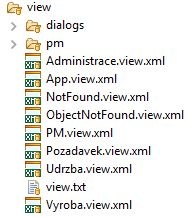
\includegraphics[]{images/fiori_app_view_struct}
	\caption{Struktura jednotlivých view v Eclipse projektu}
	\label{img:views_strucutre}
\end{figure}
\begin{figure}[H]
	\centering
	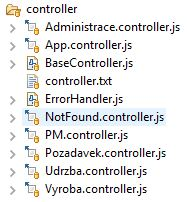
\includegraphics[]{images/fiori_app_controller_struct}
	\caption{Struktura controllerů v Eclipse projektu}
	\label{img:controlllers_structure}
\end{figure}
Jak je z obrázků patrné, view mají zpravidla stejnojmenný protějšek v controllerech. To je z toho důvodu, že každé view má přiřazen jeden controller a z důvodu přehlednosti jsou proto pojmenovány stejně. 

\subsubsection{App}
\label{sssec:fiori_app}
Není ani tak stránkou jako spíš základním view aplikace. V podstatě pouze všechny ostatní view obaluje a svůj obsah dynamicky střídá na základě uživatelových kroků. Je nastaveno jako výchozí pro všechny možné kombinace URL, které je uživatel v rámci aplikace schopen vytvořit.
\paragraph{View} View je zadefinováno způsobem zobrazeném v následujícím kódu \ref{code:view_app_definition}.
\begin{algorithm}[H]
	\begin{lstlisting}[language=xml]      
<mvc:View controllerName="sap.ui.mo.pm.controller.App"
          xmlns="sap.m" xmlns:mvc="sap.ui.core.mvc" >
  <App id="app" />
</mvc:View>
	\end{lstlisting}
	\caption{XML definice view App}	
	\label{code:view_app_definition}
\end{algorithm}	
Definice neříká nic jiného, než ze v případě zobrazení tohoto view má být vnořena standardní SAPUI5 komponentu App, která slouží jako základ aplikace. V rámci této komponenty jsou následně agregována view popsaná dále. Jak je v kódu vidět, je zde parametr \uv{controllerName}, který přiřazuje k view controller. 
\paragraph{Controller} Stejně jako v ostatních případech je z důvodu přehlednosti totožně pojmenován. Jedinou jeho funkčností je v první fázi spouštění apliakce nastavit dále neměnně atributy. Jak je vidět v ukázce kódu \ref{code:controller_app_definition} níže, dochází zde k nastavení výchozího jazyka aplikace a kaskádových stylů v závislosti na typu použitého zařízení. Jiné styly jsou tak použity pro zařízení s rozlišením odpovídající tabletům, mobilů, nebo desktopům. V potaz se bere i dotykový displej, vyžadující si například větší tlačítka než by tomu bylo v případě použití obyčejného monitoru.
\begin{algorithm}[H]
	\begin{lstlisting}[language=java]      
BaseController.extend("sap.ui.pm.controller.App",{
  onInit : function() {
    sap.ui.getCore().getConfiguration().setLanguage("cs");
    var component = this.getOwnerComponent();
    var css = component.getContentDensityClass();
    this.getView().addStyleClass(css);
  }
}; 
	\end{lstlisting}
	\caption{XML definice view App}	
	\label{code:controller_app_definition}
\end{algorithm}	
Za zmínku ovšem stojí i první řádek zobrazeného kódu \ref{code:controller_app_definition} výše. Výraz \uv{BaseController.extend("sap.ui.mo.pm.controller.App"} říká, že nedochází k rozšíření standardního controlleru frameworku, ale v tomto případě k aplikaci přiloženému controlleru pojmenovaného \uv{BaseController}.
\paragraph{BaseController} Od tohoto controlleru odvozuji všechny ostatní implementované. To protože se nemalá část funkcí dá využít na více místech v aplikaci a nemusí tak docházet k duplikování kódu, které by přinášelo riziko snížení konzistence a zvýšení pracnosti v případě budoucích změn nebo opravování chyb. Tento controller je již odvozen od standardního frameworkového controlleru \uv{sap.ui.core.mvc.Controller}. 
Následující ukázka kódu \ref{code:controller_base_definition} zobrazuje tři takové společné funkce. Celý výčet je pochopitelně mnohem delší, ale tyto  byly vybrány, protože jsou nejčastěji používané a poslouží tak k dobré demonstraci snížené pracnosti a náročnosti na údržbu aplikace z pohledu vývojáře. Funkce zobrazené v ukázce kódu \ref{code:controller_base_definition} jsou posléze krátce popsány.
\begin{algorithm}[H]
	\begin{lstlisting}[language=java]      
Controller.extend("sap.ui.pm.controller.BaseController",{

  createDialog : function(that, id, dialog, fragment) {
    if (!dialog) {
      var frag = sap.ui.xmlfragment(id, fragment, that);
      that.getView().addDependent(frag);
      jQuery.sap.syncStyleClass("sapUiSizeCompact", 
                                that.getView(), res);
      return frag;
    }
    return dialog;
  },  
  
  setModel : function(oModel, sName) {
    return this.getView().setModel(oModel, sName);
  },

  getI18NText : function(that, id) {
    var oModel = that.getView().getModel("i18n");
    var oBundle = oModel.getResourceBundle();
    return oBundle.getText(id);
  }, 
}; 
	\end{lstlisting}
	\caption{XML definice view App}	
	\label{code:controller_base_definition}
\end{algorithm}	

\begin{itemize}
	\item
	\textbf{createDialog}: Aby mohly být v rámci controlleru vytvářeny jednotlivé dialogy (až desítky na jeden controller) téměř bezpracně, byla vytvořena následující prototypová funkce vytvářející v požadovaném controlleru objekt reprezentující dialog. K vytvoření takového dialogu poté stačí jeden příkaz jako v ukázce \ref{code:create_dialog} níže. 
\begin{algorithm}[H]
	\begin{lstlisting}[language=java]      
that.oEqunrSTD = that.createDialog(that, that.oEqunrSTD,
   "../view.dialogs.EqunrSelectTreeDialog");
	\end{lstlisting}
	\caption{Ukázka kódu pro vytvoření objektu dialogu}	
	\label{code:create_dialog}
\end{algorithm}		
	\item
	\textbf{setModel}: Slouží k provázání modelu (objekt obsahující data) s požadovaným view. Každá UI komponenta frameworku umožňuje svázání s modelem a jeho konkrétním prvkem. V případě přeřazení takového modelu k view pak může dojít k zobrazení požadované hodnoty. Jelikož svazování dat v modelu s view patří k velmi častým operacím a vyžaduje volání více funkcí, je obaleno do této metody, které stačí předat jako parametr požadovaný model a jeho jméno.
	\item
	\textbf{getI18NText}: Velmi často v controlleru dojde k situaci, že je potřeba uživateli sdělit nějakou informaci. Může se jednat například o dialogové okno nebo jenom probliknutí textu informujícího o provedené nějaké akce. Aby v controlleru nebyly ošetřovány situace aktuálního jazyka a podobně, je vytvořena tato funkce, která načte hodnotu prvku v aktuálním používaném jazyce z příslušného internacionalizačního souboru. 
\end{itemize}	

\subsubsection{PM - Úvodní stránka}
\label{sssec:fiori_pm}
Reprezentuje úvodní obrazovku, jejíž obsah je přímo závislý na rolích, které má uživatel k dispozici. Zde bude uživateli kromě otevření aplikací umožněno změnit si heslo.
\paragraph{View}
Pro demonstraci struktury jednotlivých view je v této, jakožto první, ukázce obsahující větší počet komponent zobrazena téměř celá XML struktura rozdělena do tří bloků. V implementaci 
\begin{algorithm}[H]
	\begin{lstlisting}[language=xml]      
<Page>
  <customHeader>
    <Bar design="Header">
      <contentLeft />
      <contentMiddle>
        <Title text="{i18n>pmPageTitle}"  />
      </contentMiddle>
      <contentRight>
        <Button icon="://key" press="onEditPassword" />
        <Button icon="://log" press="onLogout" />
      </contentRight>
    </Bar>
  </customHeader>
	\end{lstlisting}
	\caption{XML definice hlavičky úvodní stránky}	
	\label{code:view_pm_header_definition}
	\small Ve všech aplikacích se jedná o lehkou modifikaci této struktury. Zpravidla dochází ke změnám pouze u svazování nadpisu a použitých tlačítkách v horní liště. Jak lze vykoukat, hlavičková lišta je rozdělena do tří částí, které lehce umožňují zarovnání použitých komponent.
\end{algorithm}	
\begin{algorithm}[H]
	\begin{lstlisting}[language=xml]      
  <VBox width="100%" justifyContent="Center" >
    <l:Grid id="gridContainer" defaultSpan="L3 M6 S6" />
  </VBox>
	\end{lstlisting}
	\caption{XML definice obsahu úvodní stránky}	
	\label{code:view_pm_content_definition}
	\small Jak je v ukázce vidět, jedná se o velmi jednoduchý obsah stránky. V podstatě je pouze zadefinováno rozložení Grid kontejneru, které má implicitně responzivní chování. Vývojář tedy nemusí nijak extra řešit počet zobrazených agregovaných komponent, framework to zvládá sám.  
\end{algorithm}	
\begin{algorithm}[H]
	\begin{lstlisting}[language=xml]      
</Page>
	\end{lstlisting}
	\caption{XML definice zápatí úvodní stránky}	
	\label{code:view_pm_footer_definition}
	\small V tomto případě se jedná pouze o ukončení stránky. U ostatních aplikací mohou být zobrazovány například různá zápatí obsahující tlačítka s funkcemi a podobně.
\end{algorithm}	
\paragraph{Controller} Má v rámci této stránky primární úkol k přidělené požadovaných dlaždic uživateli v závislosti na přidělených rolích. To spočívá v načtení uživatelských rolí a přidání dlaždic do Grid kontejneru zadefinovaného v ukázce kódu \ref{code:view_pm_content_definition} výše. 
\paragraph{Stránka} Výsledná podoba stránky je zobrazena na obrázku \ref{img:view_pm} níže. Jedná se o velmi minimalistické provedení, jelikož se neočekává, že by zde uživatel trávil větší množství času. Obrázek je rozdělen na dvě části. V první je podoba stránky zobrazené v běžném desktop rozlišení (více jak 1200 pixelů na šířku). V druhé části je zobrazena podoba v mobilním zařízení odpovídajícímu dnešnímu standardnímu chytrému telefonu s obrazovkou velkou přibližně 5 palců (šířka alespoň 350 pixelů na šířku).
\begin{figure}[H]
	\centering
	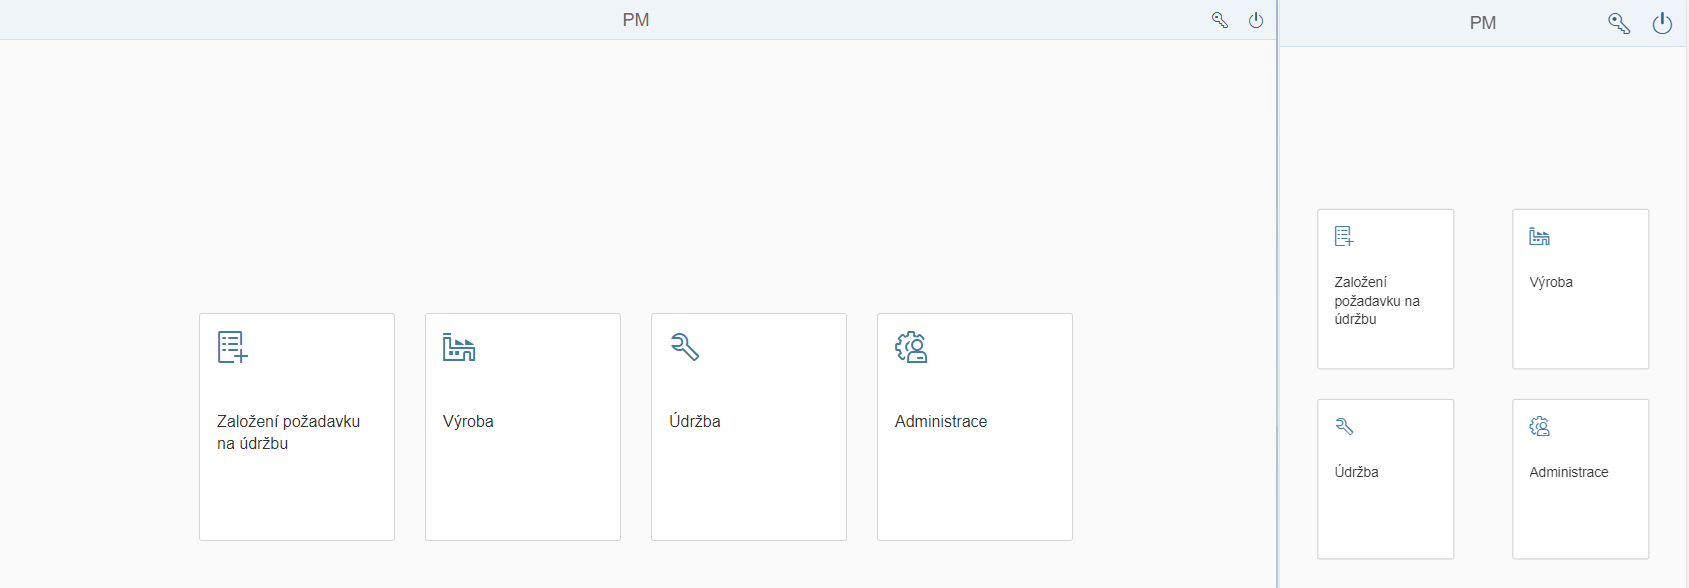
\includegraphics[width=1\textwidth]{images/view_pm}
	\caption{Úvodní stránka PM SAPUI5 aplikace}
	\label{img:view_pm}
	\small Podoba stránky odpovídá případu, kdy má uživatel přiřazené všechny dosavadní role.
\end{figure}

\subsubsection{Pozadavek - Založení požadavku na údržbu}
\label{sssec:pozadavek}
Stránka je navržena tak, aby odpovídala funkčnímu požadavku \ref{sssec:fc_zalozeni_pozadavku}. Je zde proto vytvořen formulář umožňující zadat veškeré potřebné údaje ke specifikování požadavku. 
\paragraph{View}
Jelikož se jedná v podstatě pouze o formulář určený k vyplnění od uživatele, je obsahem view především komponenta SimpleForm, pomocí které lze snadno vytvořit cílený formulář. 
\begin{algorithm}[H]
	\begin{lstlisting}[language=xml]      
<f:SimpleForm>
  <Label text="{i18n>pozadavekTplnrLabel}" />
  <Input value="{hlaseni>/tplnr}" showValueHelp="true" 
         valueHelpRequest="onTplnrMatchCodeRequest" />
  <ndc:BarcodeScannerButton scan="handleScan" />
  <Label text="{i18n>pozadavekVybaveniLabel}" />
  <Text text="{hlaseni>/eqktx}" />
</f:SimpleForm>
	\end{lstlisting}
	\caption{XML definice obsahu úvodní stránky}	
	\label{code:view_pozadavek_form}
	\small Komponenta SimpleForm vytváří formulář na základě komponenty Label, která od sebe jednotlivé části separuje. Všechny elementy od Labelu až k dalšímu tvoří jeden celek a jsou výsledně rendrovány v jedné skupině.
\end{algorithm}	
\paragraph{Controller}
Úkolem controlleru na této stránce je především předvyplnění uživatelských atributů do vstupního formuláře a jeho následné odeslání na backend. To spočívá v načtení uživatelských dat v případě navštívení stránky s následným  naplnění modelu příslušnými daty. Obsahuje také funkce pomáhající uživateli vybrat data. Takovým příkladem může být načtení hierarchie technických míst. K tomu je zapotřebí poslat požadavek pro data. K tomu poslouží funkce query implementující AJAX request \ref{code:ajax} v JavaScriptové knihovně utils. Předáním lokálních funkcí pro úspěšné a neúspěšné volání poté může dojít zpracování přijatých dat nebo chyb. Pomocí funkce setModel popsané v BaseControlleru \ref{code:controller_base_definition} a nebo přístupem ke konkrétnímu prvku modelu (funkce setProperty) lze potom nastavit požadovaná data do svázaného formuláře. 
\paragraph{Stránka}
Výsledná stránka je reprezentována formulářem o sedmi prvcích. Podle typu zadávaných hodnot v poli je pak přizpůsobena komponenta ulehčující uživateli vyplnění. Pro technické místo je možné si nechat zobrazit dialog s hierarchií technických míst a vybavení si z něho vybrat. U elementů s pevně daným výběrem a zároveň striktně omezeným počtem je pak vybrána komponenta SelectList a podobně. Podoba stránky pro desktop a mobilní zařízení je vidět na obrázku \ref{img:view_zalozeni_pu} níže.
\begin{figure}[H]
	\centering
	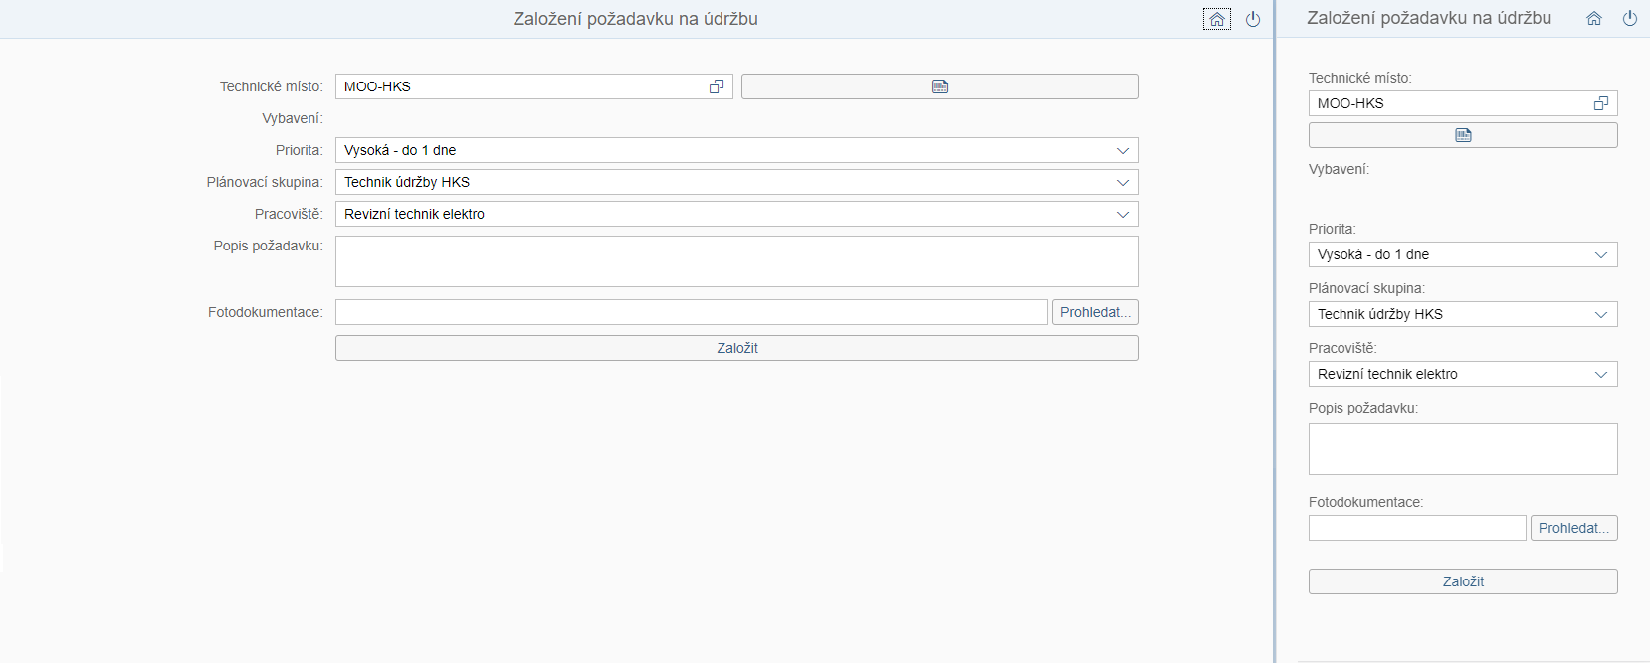
\includegraphics[width=1\textwidth]{images/view_zalozeni_pu}
	\caption{Stránka pro založení požadavku na údržbu}
	\label{img:view_zalozeni_pu}
\end{figure}

\subsubsection{Vyroba - Operátor výroby}
\label{sssec:fiori_vyroba}
Stránka je navržena tak, aby odpovídala funkčním požadavkům spadající pod roli Operátora výroby. Musí zde tedy býti dostupný seznam jednotlivých hlášení (poruchy, prevence a údržby) pro jeho přidělené pracoviště. V rámci jednotlivých hlášení je zapotřebí mít k dispozici relevantní operace, které s nimi operátor může provést.
\paragraph{View}
Z důvodu responzibility se jedná o první stránku, kde je zapotřebí již v rámci view řešit rozlišení používaného zařízení z důvodu obsáhlé tabulky, která se na mobilních zařízeních nebude vhodně zobrazovat. V horní části obrazovky jsou navrženy dva filtry. První z nich je na typ zobrazovaného hlášení a druhým je filtr na technická místa. Filtr přes druh hlášení nejen, že filtruje data, ale i mění zobrazované informace. Požadovaná zobrazovaná data k jednotlivých typům hlášením nejsou totiž identická. Tato část je pro desktopová i mobilní zařízeni stejná. Dále se však struktura stránky liší. 
\paragraph{View (desktop)}
Pod filtry je navržena tabulka se všemi možnými sloupci, které se mohou v rámci stránky zobrazit. V rámci jednotlivých sloupců jsou pak přiděleny agregace na UI komponenty vyhovujícím požadavkům. Jedná se především o texty a tlačítka, která jsou zobrazována v závislosti na stavu (statusu) hlášení. O logiku se stará knihovna utils \ref{file:utils.js} implementující funkce rozhodující o informaci zobrazit nebo nezobrazit.
\paragraph{View (mobile)}
Pod filtry je navržen komplikovanější rozložení skládající se z desítek komponent různých layoutů uspořádaných do hierarchické struktury. Bylo zapotřebí změnit celou strukturu oproti tabulkovému zobrazení. Každé hlášení tak horizontálně zabírá více místa. Namísto maximálně dvou řádků v rámci jednoho hlášení se tak nyní vyskytuje až sedm řádků informací.
\paragraph{Controller}
Kromě standardních činností, jako je odchytávání uživatelovi interakci s patřičným zpracováním, je zde zapotřebí dynamicky řešit obsah hlavního view. Toho je dosaženo za pomocí modelu zařízení a \textbf{návrhového vzoru pozorovatel}, který řeší informování požadovaných objektů o změně stavu jiného objektu. Pozorovaným objektem je v tomto případě model zařízení (konkrétně jeho část řešící aktuální rozlišení). Pozorovatelem je objekt (funkce) controlleru. Jelikož je tabulka společná pro všechny druhy hlášení, řeší controller zobrazení jednotlivých sloupců. 
\begin{algorithm}[H]
	\begin{lstlisting}[language=java]     
var dev = this.getOwnerComponent().getModel("device");
dev.getProperty("/resize").attachHandler(this.onResize);
	\end{lstlisting}
	\caption{Přiřazení posluchače ve formě funkce k hodnotě modelu}	
	\label{code:resize_attach_handler}
	\small Jedná se o výtažek kódu v inicializační funkci onInit. Spočívá v načtení device modelu a přiřazení posluchače v podobě funkce onResize, která se provede vždy při změně rozlišení. To znamená zahrnuje i případ otočení displeje na mobilních zařízeních.
\end{algorithm}	
\begin{algorithm}[H]
	\begin{lstlisting}[language=java]      
onResize : function(window) {
  var layout = that.getView().byId("notifLayout");
  layout.removeAllContent();
  if (window.width > 1024) {
    layout.addContent(that.notifTable);
  } else {
    layout.addContent(that.notifList);
}
	\end{lstlisting}
	\caption{Implementace funkce onResize}
	\label{code:resize_handler}
	\small Jako hraniční hodnota pro zobrazení tabulky nebo listu byla vybrána hodnota 1200 pixelů. V případě změny dojde k odebrání fragmentu z layoutu a přiřazení adekvátního obsahu.
\end{algorithm}	
\paragraph{Stránka}
Cílem návrhu této stránky bylo maximální možné eliminování tlačítek a textů, které uživatel nepotřebuje znát. Tudíž všechny texty i tlačítka se zobrazují v případě, že mají nějaký význam. U textů to jsou pro uživatele potřebné informace k vykonávání jeho práce. V případě tlačítek umožňujících akce nad daným hlášením je tento problém řešen zobrazením jenom těch tlačítek, které lze nad daným hlášením v danou chvíli provést. Zrušit hlášení tak lze pouze do doby, než s ním někdo začne pracovat. Zobrazovat texty k hlášení jdou pouze tehdy, když už nějaký text k němu existuje a podobně. Podoba stránky pro desktop a mobilní zařízení je vidět na obrázku \ref{img:view_vyroba} níže.
\begin{figure}[H]
	\centering
	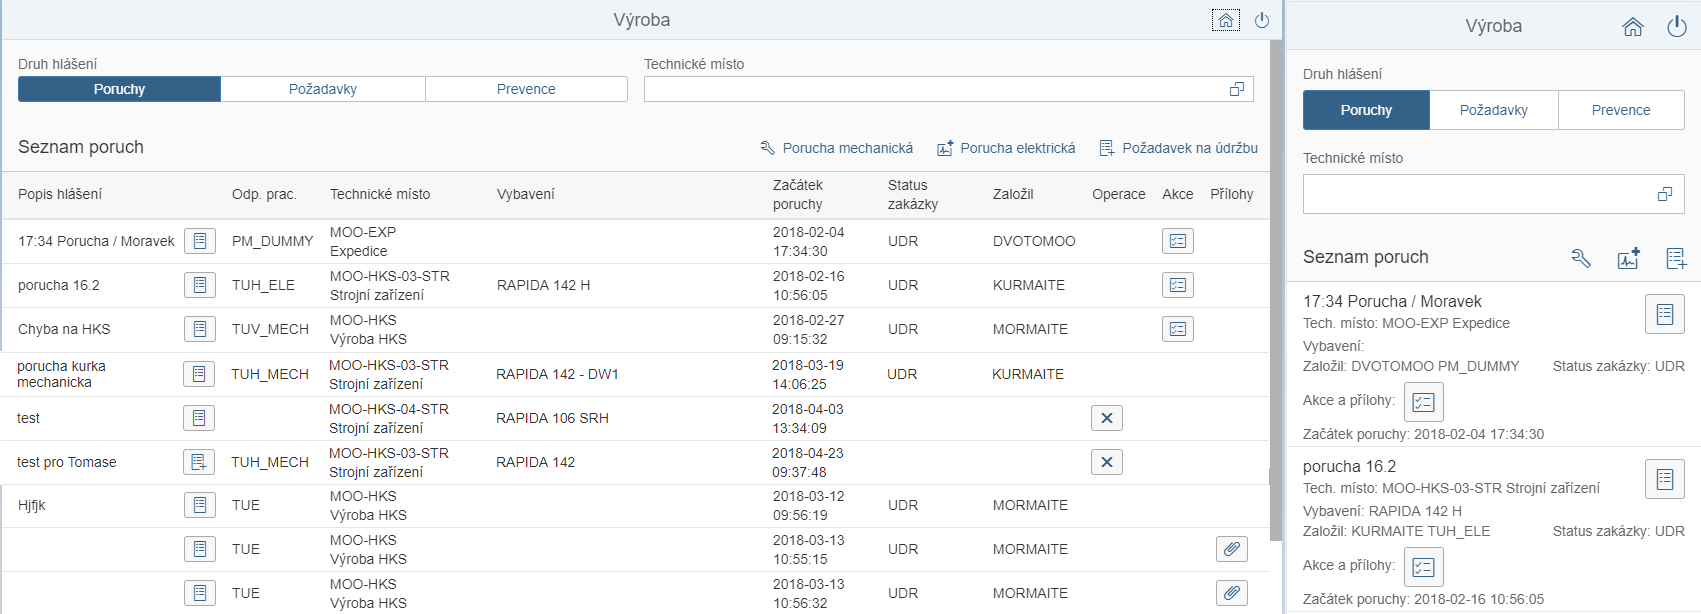
\includegraphics[width=1\textwidth]{images/view_vyroba}
	\caption{Stránka pro operátora údržby}
	\label{img:view_vyroba}
\end{figure}

\subsubsection{Udrzba - Údržbář}
\label{sssec:fiori_udrzba}
Stránka je navržena tak, aby odpovídala funkčním požadavkům spadající pod roli Údržbáře. Musí zde tedy býti dostupný seznam jednotlivých hlášení (poruchy, prevence a údržby) připravených k provedení servisního úkonu. V rámci jednotlivých hlášení je zapotřebí mít k dispozici relevantní operace, které s nimi údržbář může provést.
\paragraph{View}
Jelikož je seznam jednotlivých druhů hlášení řešen pomocí tabulky, stejně jako v případě operátora výroby \ref{sssec:fiori_vyroba}, je opět přistoupeno k oddělení jednotlivých view na fragmenty, které se v závislosti na šířce e používaného zařízení přidávají a odebírají. Oproti stránce pro operátory výroby je zde ale požadovaných funkcionalit trochu více a proto je rozdělení typů hlášení řešeno jinak. Místo přepínacího filtru mezi poruchami, prevencemi a údržbami vzniklo pět záložek. Tři z nich kopírují druhy hlášení, zbylé dvě slouží pro dohledání dokumentace k vybavení a zobrazení historie poruch.
\paragraph{View (desktop)}
Všech pět záložek je řešeno pomocí tabulek s různými sloupci. Požadavek na minimální počet zobrazených elementů zůstává. A i zde jsou proto texty a tlačítka zobrazována na základě knihovny utils \ref{file:utils.js}. 
\paragraph{View (mobile)} 
Všech pět záložek je realizováno pomocí různých layoutů uspořádaných do hierarchické struktury komponent. 
\paragraph{Controller}
Kromě standardních činností, jako je odchytávání uživatelovi interakci s patřičným zpracováním, je zde zapotřebí dynamicky řešit obsah hlavního view. Toho je dosaženo za pomocí modelu zařízení a \textbf{návrhového vzoru pozorovatel}, který řeší informování požadovaných objektů o změně stavu jiného objektu. Pozorovaným objektem je v tomto případě model zařízení (konkrétně jeho část řešící aktuální rozlišení). Pozorovatelem je objekt (funkce) controlleru. Jelikož je tabulka společná pro všechny druhy hlášení, řeší controller zobrazení jednotlivých sloupců. 
\paragraph{Stránka}
Stránka je řešena trochu odlišně než tomu je u operátory výroby \ref{sssec:fiori_vyroba}. Místo filtru nad druhem hlášení jsou navrženy jednotlivé záložky s tím, že každá má přidělenou svoji adekvátní tabulku. Podoba stránky pro desktop a mobilní zařízení je vidět na obrázku \ref{img:view_vyroba} níže.
\begin{figure}[H]
	\centering
	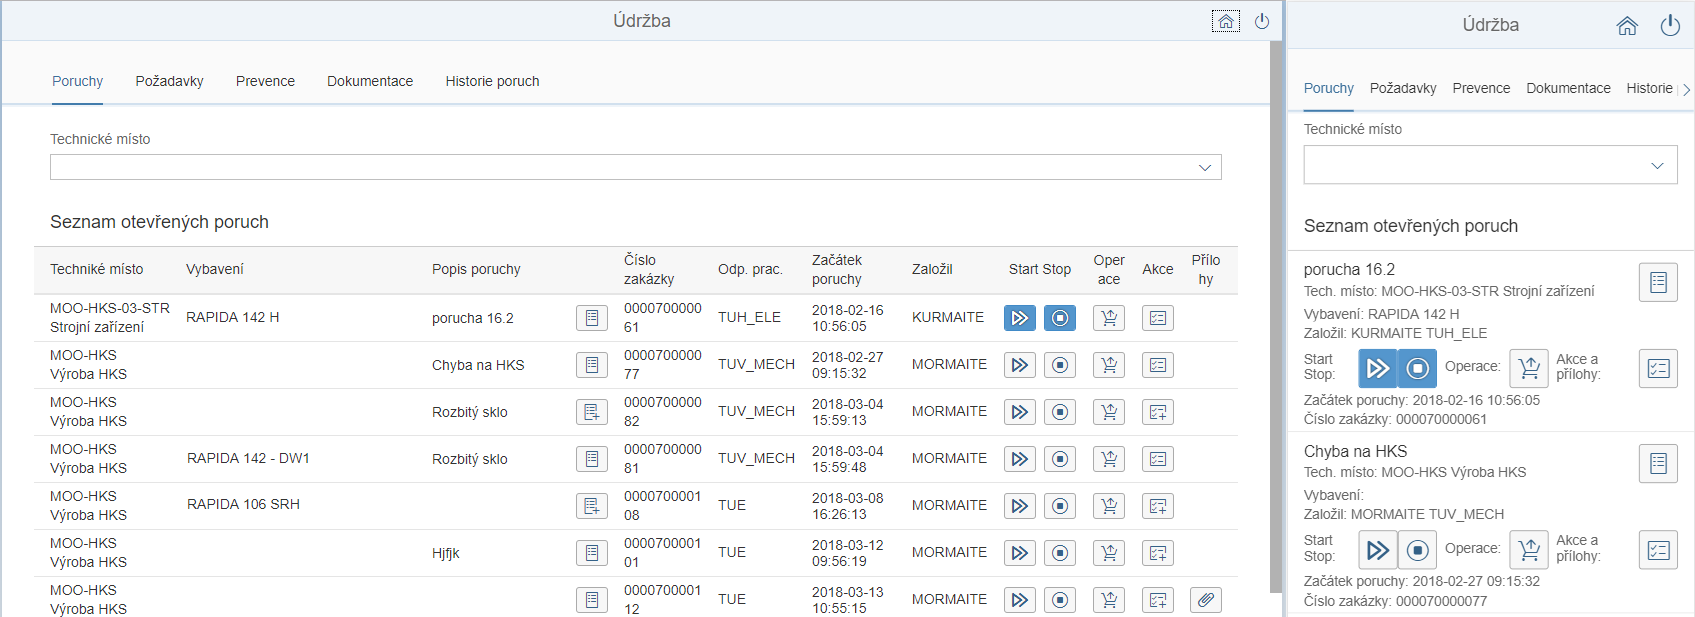
\includegraphics[width=1\textwidth]{images/view_udrzba}
	\caption{Stránka pro údržbáře}
	\label{img:view_udrzba}
\end{figure}	

\subsubsection{Administrace}
\label{sssec:fiori_administrace}
Stránka je navržena tak, aby odpovídala funkčním požadavkům spadající pod roli Administrátora. Musí zde být k dispozici seznam všech uživatelů a umožněno provádět nad jednotlivými uživateli požadované operace jako je editace atributů, rolí nebo jména a hesla uživatele.
\paragraph{View}
Administrace používá koncepčně trochu jiný typ přístup než předchozí stránky. Je zde použita komponenta SplitApp pomyslně rozdělující stránku na master a detail část. Ačkoli to není nutné, obecně se v master části očekává libovolný seznam prvků, jejichž výběrem se v detail části zobrazí podrobné informace příslušného prvku. V tomto případě se tak jedná o seznam uživatelů pro master část a jeho podrobné informace v detail části. Pro seznam je použita standardní listová komponenta obsahující pouze název uživatelského účtu. V detailní části je potom v hlavičce osobní číslo a jméno uživatele a pod tím záložky pro pracoviště, role a atributy. Struktura této stránky je k vidění v ukázce kódu \ref{code:split_app} níže. 
Rozdílné chování je znát i na mobilních zařízeních. Master a Detail stránky jsou v tomto případě rozděleny a chovají se jakoby samostatné stránky, ačkoliv je za nimi schován jeden controller a sdílí všechny data tak, jako by jednou stránkou byly. 
\begin{algorithm}[H]
	\begin{lstlisting}[language=java]      
<SplitApp initialDetail="detailDefault" 
          initialMaster="master">
  <masterPages>
    <Page id="master" >
      <customHeader /> 
      <content />
      <footer />
    </Page>
  </masterPages>
  <detailPages>
    <Page id="detailDefault">
      <customHeader /> 
      <content />
      <footer />
    </Page>
    <MessagePage id="detailNotFound" />
  </detailPages>
</SplitApp>
	\end{lstlisting}
	\caption{}
	\label{code:split_app}
	\small Ukázka má nastínit základní strukturu SplitApp komponenty. Základním stavebním kamenem jsou agregace masterPages a detailPages. Těm lze přiřadit libovolný počet komponent typu Page, jejichž struktura byla už dříve zmíněna v kapitole \ref{sssec:fiori_pm}.
\end{algorithm}	
\paragraph{Controller}
Oproti předchozím controllerům zde musí být implementováno chování pro správný chod SplitApp aplikace. To obnáší vyčítání parametrů z URL z důvodu zjištění, jestli je nějaký konkrétní uživatel již vybrán. Příkladem může být cesta \uv{/pm/\#/administrace/MORMAITE)}, ze které lze poznat vybraný uživatelský účet MORMAITE a na základě toho z backendu získat příslušná data. Ale to se netýká pouze načítání dat. Je zapotřebí pro případ mobilních zařízení rozlišit, zdali má být zobrazena master nebo detail stránka. Pro to však lze nastavit jednoduché pravidlo. V případě, že je účet znám (například URL \uv{/pm/\#/administrace/MORMAITE)}), dojde k zobrazení detailu, jinak master části se seznamem uživatelů k výběru (například URL \uv{/pm/\#/administrace/)}).
\paragraph{Stránka}
Pro stránku byl zvolen rozdělené layout, který zřetelně odděluje seznam uživatelů od jejich detailu. V zápatí seznamu je tlačítko pro založení nového uživatele realizovaného pomocí formuláře zobrazeného v dialogovém okně. V detailní části jsou pak zobrazené všechny požadované informace. Lze tak tedy například editovat osobní číslo a jméno uživatele. V záložkách jsou potom tabulky jednotlivých pracovišť, rolí a atributů, které může správce editovat. Podoba stránky pro desktopzařízení je vidět na obrázku \ref{img:view_administrace} níže.
\begin{figure}[H]
	\centering
	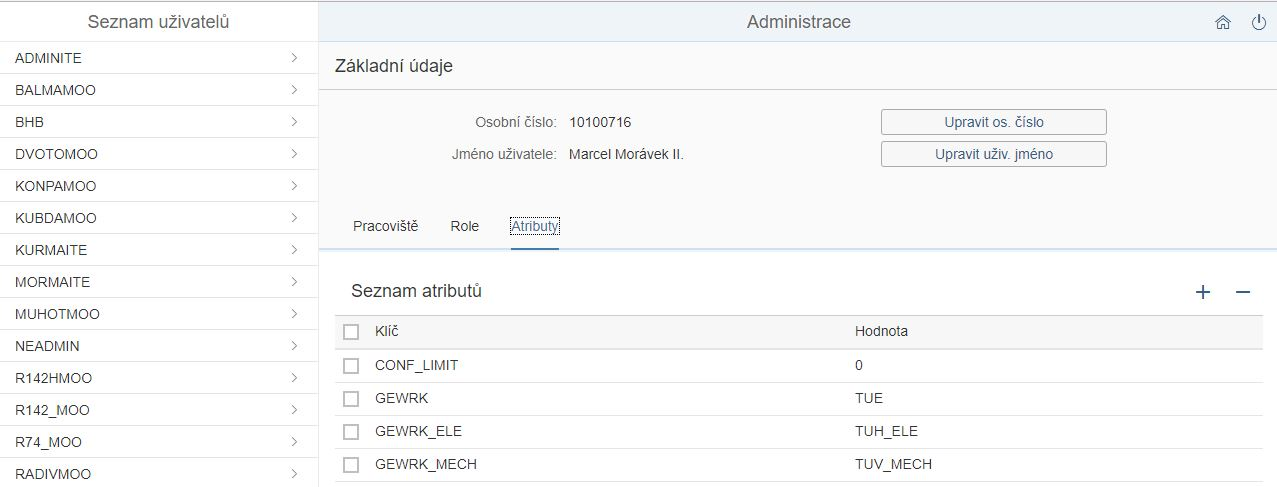
\includegraphics[width=1\textwidth]{images/view_administrace}
	\caption{Stránka pro správu uživatelů}
	\label{img:view_administrace}
\end{figure}	
Stránka pro mobilní verzi je z důvodu rozdělení tentokrát zobrazena samostatně na obrázku \ref{img:view_administrace_mob} níže. Z důvodu zpětné navigace z detailu do seznamu přibila v hlavičce šipka zpět pro vykonání tohoto úkonu. Jinak je vzhled víceméně totožný s verzí pro destop zařízení.  
\begin{figure}[H]
	\centering
	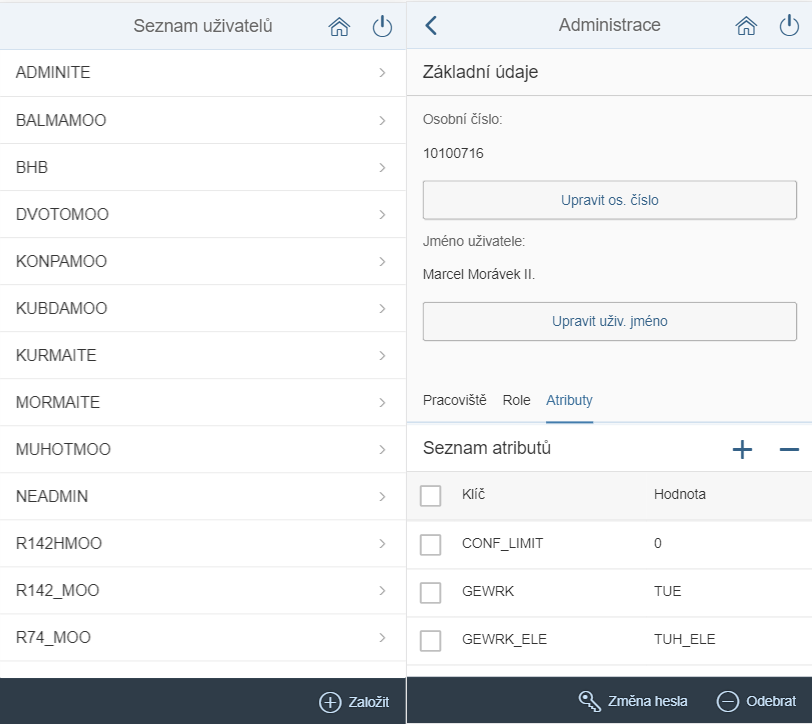
\includegraphics[width=0.6\textwidth]{images/view_administrace_mob}
	\caption{Stránka pro správu uživatelů - mobilní verze}
	\label{img:view_administrace_mob}
\end{figure}	

\subsubsection{Pomocné dialogy}
V rámci aplikace vznikly přibližně tři desítky různých dialogů sloužící pro různé účely. Ty nejjednodušší z nich mají například jednoduchý účel vyžádání potvrzení úkonu od uživatele před provedením. Údržbář je například při ukončení práce dotázán, zdali chce svoji předat operátorovi výroby ke schválení. Tím dojde k omezení chyb vzniklých z důvodů neopatrnosti. Vznikly však i dialogy trochu komplikovanější. Zpravidla se jedná o dialogy vyžadující od uživatele vyplnění nějakých dat potřebných pro provedení daného úkonu. Na obrázku \ref{img:view_dialog} níže je například k vidění dialog pro vydání náhradního dílu ze skladu jak pro desktop tak mobilní zařízení. 
\begin{figure}[H]
	\centering
	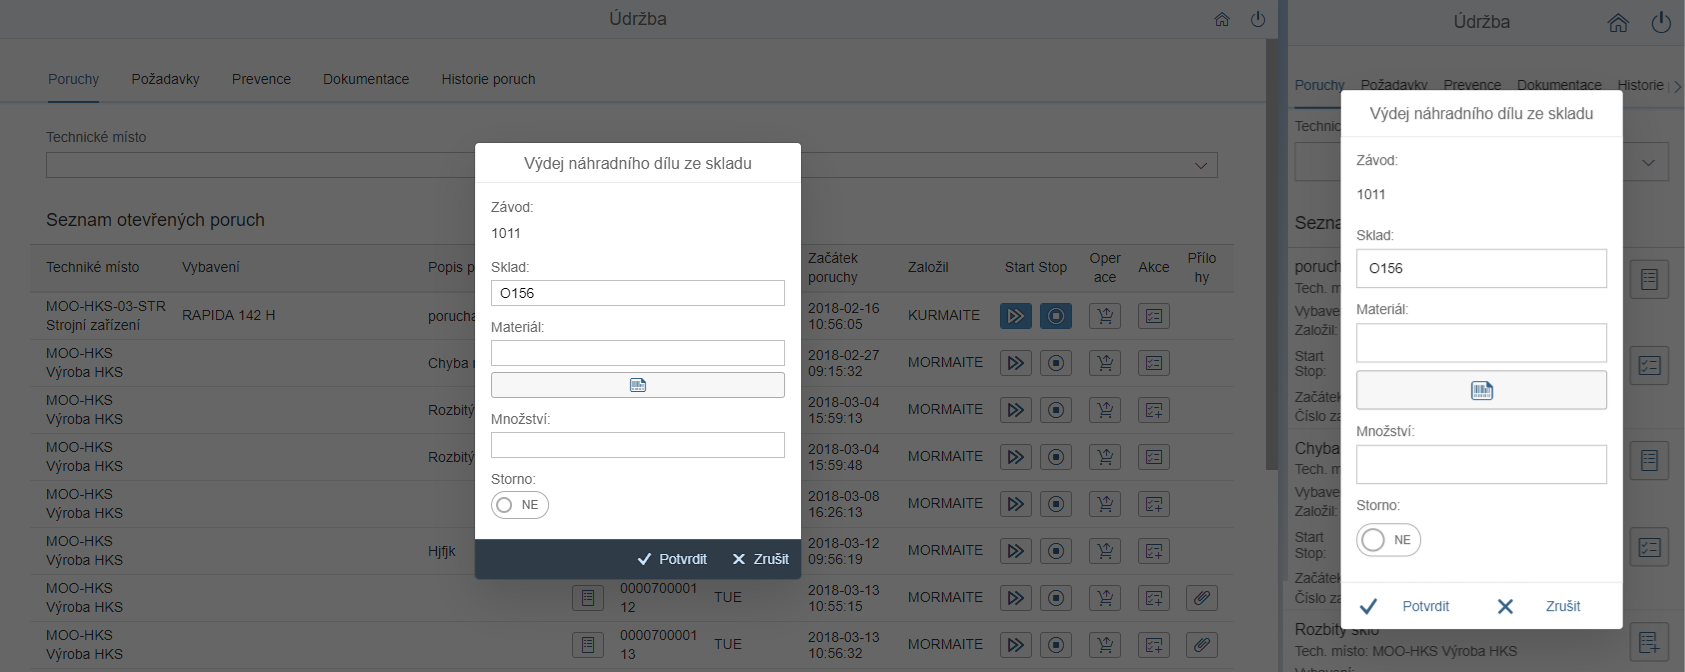
\includegraphics[width=1\textwidth]{images/view_dialog}
	\caption{Dialog pro vydání náhradního dílu}
	\label{img:view_dialog}
\end{figure}	

\section{LOGIN SAPUI5 Aplikace}
\subsection{Struktura aplikace}
Struktura aplikace je víceméně totožná s aplikací PM popsané v kapitole \ref{ssec:struckuta_pm_aplikace} výše. Jediné, v čem se aplikace zásadně liší je její zabezpečení popsané v souboru web.xml. V kapitole \ref{ssec:login_modul} věnující se autentizačnímu a autorizačnímu mechanismu JAAS popsána nutná definice zobrazená v kódu \ref{code:j2ee_definition}. Ta je použita v aplikaci PM, ale aplikace PM ji už postrádá. Z toho důvodu nepotřebuje i další soubory týkající se zabezpečení. A to HTML stránky login.html a error.html popsané v kapitole \ref{code:auth_form_def}.
\subsection{Login}
Úkolem Login stránky je autentizace uživatele. K tomu jednoduše poslouží jednoduchý vstupní formulář pro jméno a heslo.
\paragraph{View}
Pro ten byl vybrán layout SimpleForm popsaný v ukázce \ref{code:view_pozadavek_form}. 
\paragraph{Controller}
Úkolem je především komunikace s PMLoginModulem pro zajištění autentizace uživatele. Vypořádává se také s tím, že v případě pokusu uživatele přistoupit na konkrétní stránku nebo soubor zabezpečený pomocí JAAS, nedochází k implicitnímu přesměrování na domovskou stránku, ale přímo na tu cílenou. K tomu využívá dočasné lokální uložiště prohlížeče, do kterého si při prvním pokusu o načtení uloží aktuální URL a tu se po autentizaci pokusí otevřít již dostupné aplikaci PM.
\paragraph{Stránka}
\begin{figure}[H]
	\centering
	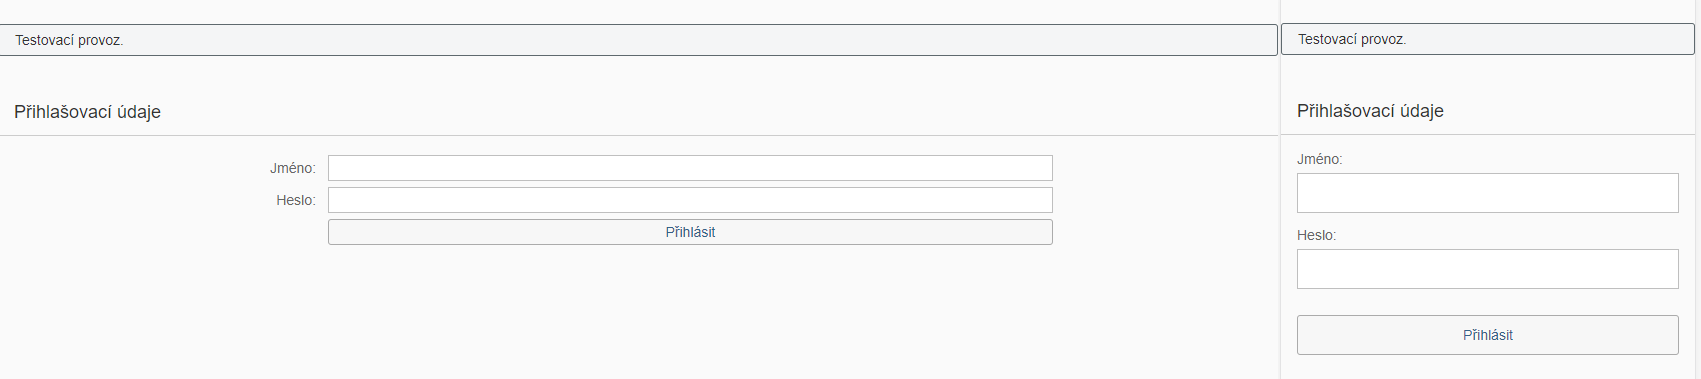
\includegraphics[width=1\textwidth]{images/view_login}
	\caption{Stránka pro přihlášení uživatele}
	\label{img:view_login}
\end{figure}

\section{Testování}
V této sekci jsou popsány testy použité při vývoji a testování dvou vrstev navržené architektury. Jedná se o vrstvu realizující prostředníka v komunikaci PM aplikace a SAP GW dále označované jako middleware a poté samotnou UI vrstvu na úrovni Fiori aplikace.

\subsection{Middleware}
Pro ukázku testovací na úrovni middleware jsem zvolil test třídy GWServlet představující prostředníka v komunikaci z aplikace PM na SAP GW.  V následující ukázce kódu \ref{code:GWServletTest} je k vidění část rozhraní testovací třídy. 
\begin{algorithm}[H]
	\begin{lstlisting}[language=java]   
public class GWServletTest {
  static GWServlet instance;	
  public GWServletTest();
	
  public static void setUpClass();
  public static void tearDownClass() ;
  public        void setUp();
  public        void tearDown();
	
  public void testGetNotifList() throws Exception;
  public void testCreateNotifPU() throws Exception;
  public void testGetTplnrHierarchy() throws Exception;
                          ...
}
	\end{lstlisting}
	\caption{Rozhraní testovací třídy pro Unit testování}	
	\label{code:GWServletTest}
\end{algorithm}

Při spuštění testu dojde k vytvoření instance třídy GWServlet z metody setUpClass, která je vyvolána před provedením prvního testu. Tím dojde na servletu k vyčtení hodnot potřebných pro HTTP komunikaci se SAP GW.

Metody setUp a tearDown zajišťují nezávislost testů, jsou totiž volány mezi jednotlivými testy a jde čas pro resetování inicializování instance nebo jiných aktivit nutných pro správnost testů. 

Na následujících dvou obrázcích \ref{img:unit_test_success} a \ref{img:unit_test_error} jsou ukázky výstupu provedených jednotkových testů v prostředí Eclipse.	

\begin{figure}[H]
	\centering
	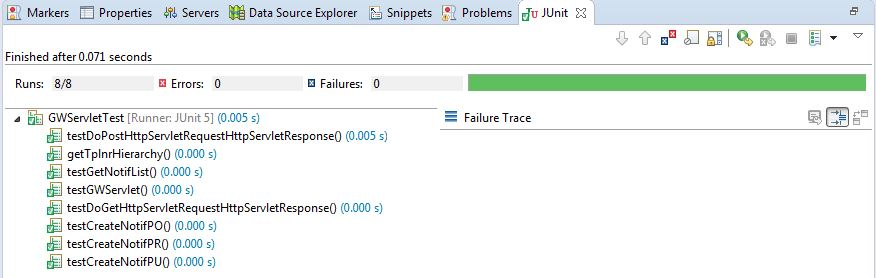
\includegraphics[width=1\textwidth]{images/unit_test_success}
	\caption{Nápověda při definování atributů elementu v SAP Web IDE}
	\label{img:unit_test_success}
\end{figure}

\begin{figure}[H]
	\centering
	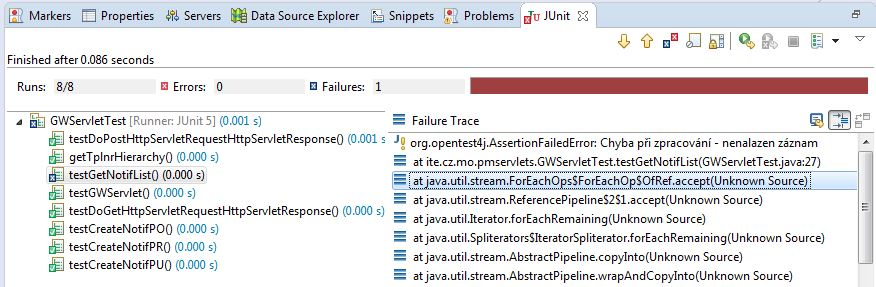
\includegraphics[width=1\textwidth]{images/unit_test_error}
	\caption{Nápověda při definování atributů elementu v SAP Web IDE}
	\label{img:unit_test_error}
\end{figure}

\subsection{UI vrstva}
K testování má framework SAPUI5 vlastní technologii OPA5 (One Page Acceptance Tests), která umožňuje testovat UI aplikace. Poskytuje asynchronní přístup k prvkům SAPUI5. Síla technologie spočívá pro testování uživatelské interakce, integraci, navigaci a svazování komponent s datovými modely. Technologie je založena na programovacím jazyku JavaScript, což je vzhledem k použití tohoto jazyka i aplikačního frameworku celkem očekávané a vhodné. V ukázce kódu \ref{code:OPA5Test} níže je k nahlédnutí struktura základního testu. 

\begin{algorithm}[H]
	\begin{lstlisting}[language=java]   
<script>
  sap.ui.require(["sap/ui/test/Opa5", ...], 
	  function (Opa5, opaTest, Common) {
    Opa5.extendConfig({ ... });
    sap.ui.require(["sap/ui/.../PM", ...], function () {
      QUnit.module("Zobrazeni detailu");
      opaTest("Prerun do detailu", function(Given, When, Then) {
        Given.iStartMyApp();
        Given.onTheIntro.iPressOnGoToDetail(); )
        When.onTheList.iPressOnGoToDetail();
        Then.onPage.iShouldSeeTheDetailPage().
        and.iTeardownMyAppFrame();
      }
    });
  QUnit.start();
});
</script>
	\end{lstlisting}
	\caption{Ukázka testovacího scriptu v hlavičce testovací stránky OPA5}	
	\label{code:OPA5Test}
	\small 
\end{algorithm}

\section{Porovnání vývojových prostředí}
V této sekci jsou popsána dvě vývojová prostředí umožňující vývoj aplikací ve frameworku SAPUI5. Prvním z nich je open source vývojové prostředí Eclipse a tím druhým je cloudové prostředí SAP Web IDE.  

\subsection{Eclipse s pluginem pro SAPUI5}
\label{ssec:eclipse_sapui5}
Eclipse umožňuje vyvíjet plnohodnotné aplikace ve frameworku SAPUI5. Jelikož ze v zásadě jedná o standardní dynamický web projekt akorát s připojenými knihovnami SAPUI5, vývoj tak probíhá dle očekávání. Umožňuje exportovat v mnoha variantách. Pro běh aplikace v Tomcat Apache je zapotřebí projekt vyexportovat do web archivu WAR. Ten poté stačí nahrát do kořenového adresáře web serveru, kde je následně rozbalen do potřebných souborů sloužících k přístupu do aplikace z webového prohlížeče. Podoba vývojové prostředí je viditelná na obrázku \ref{img:eclipse_design} níže. 
\begin{figure}[H]
	\centering
	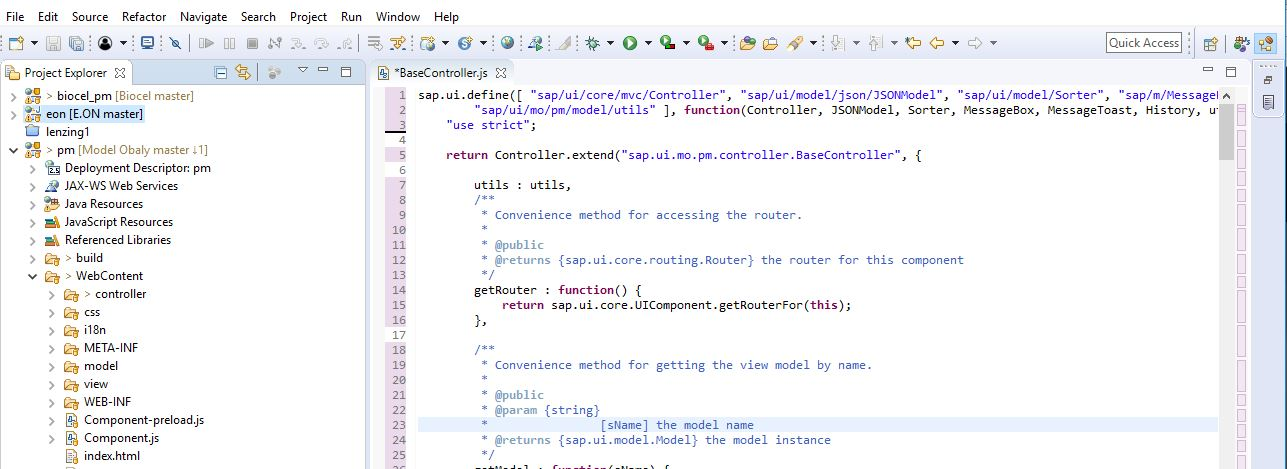
\includegraphics[width=1\textwidth]{images/eclipse_design}
	\caption{Podoba Eclipse}
	\label{img:eclipse_design}
\end{figure}
\paragraph{Prostředí} 
Vzhled a pořadí oken se dá v Eclipse libovolně měnit, nicméně v základní verzi je v levé části seznam otevřených projektů, vedle něhož je prostor pro editaci jednotlivých souborů projektu. Ve spodní části je konzole a servery dostupné pro online testování. Je možné si zde nastavit Tomcat server, který má zpracovávat a spouštět projekt. Každá úprava v kódu pak může být okamžitě zkontrolována v rámci vývojového prostředí, což je při vývoji velmi užitečné. 

\subsection{SAP Web IDE}
\label{ssec:sap_web_ide}
Reprezentuje modernější přístup k vývoji webových aplikací. Jedná se o cloudové vývojové prostředí, tudíž sdílet identické prostředí může více vývojářů současně. Kompletní vývoj je uložen ve sdíleném uložišti, které může být sdíleno do verzovacího prostředí Gitu. Nabízí širokou škálu různých dynamických funkcionalit, které pomáhají urychlit vývoj aplikace. Takovou funkcionalitou je především tvorba aplikací z předem připravených šablon. Dále se jedná o možnost rozšíření zakoupených aplikací od společnosti SAP. Zakoupená aplikace pro přehled objednávek tak může být například rozšířena o zákaznické pole u položky objednávky.

Určité omezení nastává v případě, že aplikace není cílena pro standardní nasazení očekávané od společnosti SAP. Z vývojového prostředí se očekává nahrání aplikace pouze na SAP GW. A to je znát i při vývoji aplikace z datového hlediska. V případě, že by bylo zapotřebí použít nějakou komunikační mezivrstvu (Servlet), je zapotřebí si takovou vrstvu vybudovat mimo SAP Web IDE. Standardní cestou vývoje se očekávají statické modely vytvořené v rámci aplikace nebo komunikace pomocí OData se SAP GW. 
\begin{figure}[H]
	\centering
	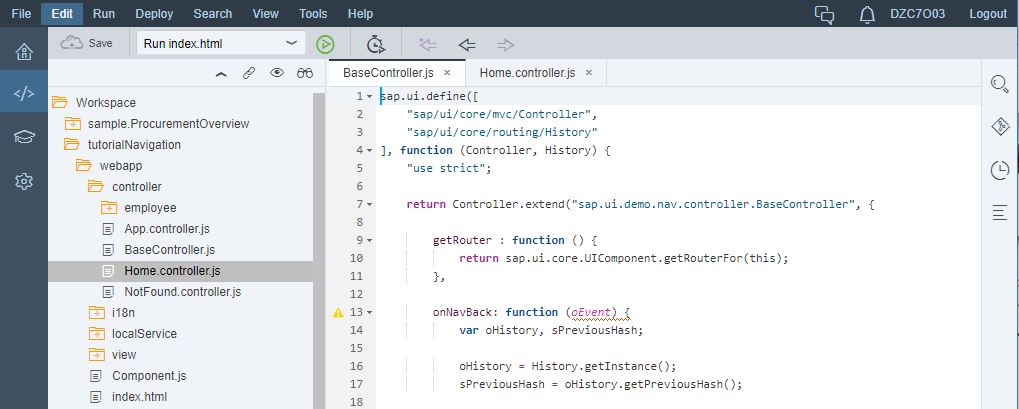
\includegraphics[width=1\textwidth]{images/web_ide_design}
	\caption{Podoba SAP Web IDE}
	\label{img:web_ide_design}
\end{figure}
\paragraph{Prostředí} Je z designového pohledu velmi elegantní, neobsahuje žádné rušivé elementy. V levé části je seznam otevřených projektů a ve zbylé části místo pro vlastní vývoj, tedy editování jednotlivých souborů. Po stranách jsou umístěné dobře viditelná tlačítka pro verzovací nástroj Git. Při psaní kódu je k dispozici nápověda ve formě doplňování názvu včetně funkcí a jejich parametrů. To však nefunguje úplně stoprocentně v rámci JavaScriptových souborů. V případě složitějších konstrukcí a volání funkcí nadřazeného objektu se nepředávají dobře návratové objekty a jejich funkce. Proto u nich nedochází k výběru volaných metod ze všech možných. Dědění z nadřazených objektů však velmi dobře pracuje u XML definic UI. 

Pro ukázku napovídání poslouží obrázky \ref{img:web_ide_help1} a \ref{img:web_ide_help2} zobrazené níže. První z nich ukazuje možnost definice tlačítka dvěma způsoby ještě před tím, než je dopsána plný název komponenty Button. První zobrazená varianta vytvoří v XML strukturu obsahující všechny atributy komponenty včetně všech možných agregací. Druhá varianta doplní pouze název komponenty. 
\begin{figure}[H]
	\centering
	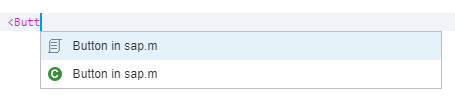
\includegraphics[width=1\textwidth]{images/web_ide_help1}
	\caption{Nápověda při výběru komponenty v SAP Web IDE}
	\label{img:web_ide_help1}
\end{figure}
U již vybrané komponenty lze však využívat nápovědu jednotlivých atributů a agregací. K výčtu jednotlivých variant je dokonce k dispozici jeho popis a vlastnosti. Ukázka je viditelná na obrázku \ref{img:web_ide_help2} níže. 
\begin{figure}[H]
	\centering
	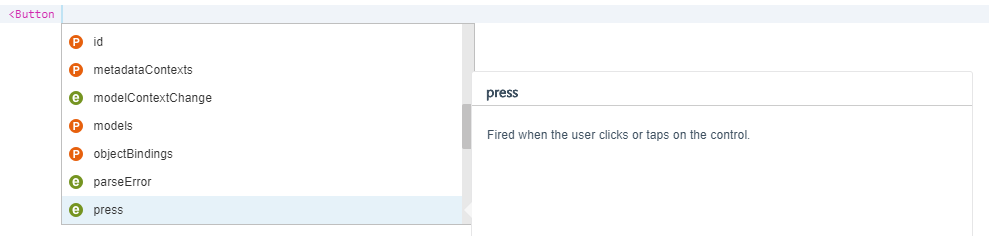
\includegraphics[width=1\textwidth]{images/web_ide_help2}
	\caption{Nápověda při definování atributů elementu v SAP Web IDE}
	\label{img:web_ide_help2}
\end{figure}

\subsection{Shrnutí}
K porovnání obou přístupů poslouží tabulka \ref{tab:eclipse_webide_comp}. Obsahuje podstatné vlastnosti zmíněné napříč sekcemi \ref{ssec:eclipse_sapui5} a \ref{ssec:sap_web_ide}. 

\begin{center}
	\begin{table}[H]
		\centering
		\begin{tabular}{| l | c | c |}
			\hline 
			Prostředí 						& Eclipse 	&	SAP Web IDE \\ 
			\hline	
			\hline
			Podpora SAPUI5					&	+		&	+			\\ 
			\hline
			Šablony pro tvorbu aplikací		&	-		&	+			\\
			\hline
			Integrace na GitHub 			&	+		&	+			\\
			\hline
			Export do WAR					&	+ 		&   -			\\
			\hline
			Online testování 				&	+		&	$\pm$		\\		
			\hline
			Připojený servlet				&	+		&	-			\\
			\hline
			Nápověda pro atributy elementů	&	-		&	+			\\
			\hline		
			Testování komunikace s GW (EPR)	&	+		&	$\pm$		\\
			\hline		
		\end{tabular}
		\caption {Tabulka shrnující vlastnosti vývojových prostředí pro SAPUI5} 
		\label{tab:eclipse_webide_comp}
	\end{table}
\end{center}

Z tabulky plusově o trochu lépe vychází varianta Eclipse. To především proto, že obecně slouží pro vývoj v jazyce Java, který se velmi často používá pro integrační účely. Tudíž tvorba pomocných servletů nebo export do Web archivu zde není problém. Kde ovšem začíná tato varianta ztrácet na síle oproti SAP Web IDE je podpora pro vývoj ve frameworku SAPUI5. Množství nápověď při skládání komponent a vypsaní controlleru k nim je v cloudu řešeno mnohem lépe. Z vývojářského pohledu ovšem postrádá možnost účinějšího testování komunikace se SAP GW oproti realizaci s middleware vrstvou implementovanou pomocí Java servletů. 

\paragraph{Doporučení} 
V závislosti na cíleném run-time prostředí, ve kterém aplikace bude nahrána, je zapotřebí vybírat vhodné vývojové prostředí. Pokud se jedná o standardní SAP GW řešení pomocí protokolu OData, pak je jednoznačně správnou volbou SAP Web IDE. V opačném případě se nejspíše očekává ohýbání standardní cesty, které s sebou přináší potřebu řešení komunikace pomocí více integrací a v tom případě se variantě zahrnující Eclipse víceméně nedá vyhnout. Víceméně vyhnout z toho důvodu, že je možné přistoupit k hybridnímu řešení. Je totiž možné UI část zahrnující XML view a JavaScriptové controllery vyvíjet v SAP Web IDE a v požadovaný moment vývoje daný projekt exportovat a nahrát do projektu v Eclipse. To lze provést buď manuální cestou exportu a importu nebo skrze verzovací systém Git. Tím lze dosáhnout uložení kódu v jednom uložišti a na konkrétních částech projektu pracovat v příslušných prostředích. UI část tak lze editovat z cloudu a část s Java vývojem a exportovacími parametry v Eclipse. 

\section{Doporučení pro vývoj}

\begin{conclusion}
Ve své práci jsem představil společnost SAP a její softwarový produkt SAP Enterprise Resource Planning. Stručně popsal význam jeho jednotlivých modulů a poté se podrobněji věnoval modulu údržby SAP Plant Maintenance. Následně jsem popsal produkt SAP Fiori a webovou technologii BSP použitou při implementaci komunikace mezi webovou aplikací a systémem SAP Gateway. 

Na základě konzultací s PM konzultantem jsem sepsal funkční požadavky kladené na výslednou aplikaci Fiori a znázornil k nim nejdůležitější případy užití. Na základě těchto požadavků jsem vytvořil návrh uživatelského rozhraní a soustředil se u něho na dodržení správných postupů návrhu. K tvorbě prototypů jsem použil dva nástroje, které jsem následně porovnal. Popsal jsem heuristickou analýzu, jakožto nástroj na určení kvality uživatelského rozhraní z důvodu vhodného použití při testování prototypu zákazníkem. 

Poté jsem na základě získaných znalostí o komponentách systému SAP, funkčních požadavcích kladených na webovou aplikaci a návrhu uživatelského rozhraní implementoval celý systém. V kapitole věnující se implementaci jsem popsal architekturu jako celek a poté podrobněji zdokumentoval její vrstvy. Nejpodrobněji je popsána část týkající se frameworku SAPUI5, kde jsou detailně popsány jeho jednotlivé stavební prvky. Poté jsou porovnána dvě vývojová prostředí uzpůsobená pro tento framework a na závěr jsem přidal ukázky možného testování uživatelského rozhraní a komunikační vrstvy tvořené Java servlety. Práce je uzavřena stručnou sadou doporučení pro budoucí vývoj aplikací v tomto frameworku.







\end{conclusion}

\bibliographystyle{csn690}
\bibliography{mybibliographyfile}

\appendix

\chapter{Seznam použitých zkratek}
% \printglossaries
\begin{description}
	\item[SAP] Systems - Applications - Products in data processing
	\item[ERP] User Interface
	\item[ABAP] Advanced Business Application Programming
	\item[GW] Gateway 
	\item[BSP] Business Server Page 
	\item[JAAS] Java Authentication and Authorization Service (Java autentizační a autorizační servus)
	\item[UI] User Interface (uživatelské rozhraní)
	\item[MVC] Model - View - Controller (Model - Uživatelské rozhraní - Řídící logika)
	\item[XML] Extensible markup language
	\item[JSON] JavaScript Object Notation
\end{description}


% % % % % % % % % % % % % % % % % % % % % % % % % % % % 
% % Tuto kapitolu z výsledné práce ODSTRAŇTE.
% % % % % % % % % % % % % % % % % % % % % % % % % % % % 
% 
% \chapter{Návod k~použití této šablony}
% 
% Tento dokument slouží jako základ pro napsání závěrečné práce na Fakultě informačních technologií ČVUT v~Praze.
% 
% \section{Výběr základu}
% 
% Vyberte si šablonu podle druhu práce (bakalářská, diplomová), jazyka (čeština, angličtina) a kódování (ASCII, \mbox{UTF-8}, \mbox{ISO-8859-2} neboli latin2 a nebo \mbox{Windows-1250}). 
% 
% V~české variantě naleznete šablony v~souborech pojmenovaných ve formátu práce\_kódování.tex. Typ může být:
% \begin{description}
% 	\item[BP] bakalářská práce,
% 	\item[DP] diplomová (magisterská) práce.
% \end{description}
% Kódování, ve kterém chcete psát, může být:
% \begin{description}
% 	\item[UTF-8] kódování Unicode,
% 	\item[ISO-8859-2] latin2,
% 	\item[Windows-1250] znaková sada 1250 Windows.
% \end{description}
% V~případě nejistoty ohledně kódování doporučujeme následující postup:
% \begin{enumerate}
% 	\item Otevřete šablony pro kódování UTF-8 v~editoru prostého textu, který chcete pro psaní práce použít -- pokud můžete texty s~diakritikou normálně přečíst, použijte tuto šablonu.
% 	\item V~opačném případě postupujte dále podle toho, jaký operační systém používáte:
% 	\begin{itemize}
% 		\item v~případě Windows použijte šablonu pro kódování \mbox{Windows-1250},
% 		\item jinak zkuste použít šablonu pro kódování \mbox{ISO-8859-2}.
% 	\end{itemize}
% \end{enumerate}
% 
% 
% V~anglické variantě jsou šablony pojmenované podle typu práce, možnosti jsou:
% \begin{description}
% 	\item[bachelors] bakalářská práce,
% 	\item[masters] diplomová (magisterská) práce.
% \end{description}
% 
% \section{Použití šablony}
% 
% Šablona je určena pro zpracování systémem \LaTeXe{}. Text je možné psát v~textovém editoru jako prostý text, lze však také využít specializovaný editor pro \LaTeX{}, např. Kile.
% 
% Pro získání tisknutelného výstupu z~takto vytvořeného souboru použijte příkaz \verb|pdflatex|, kterému předáte cestu k~souboru jako parametr. Vhodný editor pro \LaTeX{} toto udělá za Vás. \verb|pdfcslatex| ani \verb|cslatex| \emph{nebudou} s~těmito šablonami fungovat.
% 
% Více informací o~použití systému \LaTeX{} najdete např. v~\cite{wikilatex}.
% 
% \subsection{Typografie}
% 
% Při psaní dodržujte typografické konvence zvoleného jazyka. České \uv{uvozovky} zapisujte použitím příkazu \verb|\uv|, kterému v~parametru předáte text, jenž má být v~uvozovkách. Anglické otevírací uvozovky se v~\LaTeX{}u zadávají jako dva zpětné apostrofy, uzavírací uvozovky jako dva apostrofy. Často chybně uváděný symbol "{} (palce) nemá s~uvozovkami nic společného.
% 
% Dále je třeba zabránit zalomení řádky mezi některými slovy, v~češtině např. za jednopísmennými předložkami a spojkami (vyjma \uv{a}). To docílíte vložením pružné nezalomitelné mezery -- znakem \texttt{\textasciitilde}. V~tomto případě to není třeba dělat ručně, lze použít program \verb|vlna|.
% 
% Více o~typografii viz \cite{kobltypo}.
% 
% \subsection{Obrázky}
% 
% Pro umožnění vkládání obrázků je vhodné použít balíček \verb|graphicx|, samotné vložení se provede příkazem \verb|\includegraphics|. Takto je možné vkládat obrázky ve formátu PDF, PNG a JPEG jestliže používáte pdf\LaTeX{} nebo ve formátu EPS jestliže používáte \LaTeX{}. Doporučujeme preferovat vektorové obrázky před rastrovými (vyjma fotografií).
% 
% \subsubsection{Získání vhodného formátu}
% 
% Pro získání vektorových formátů PDF nebo EPS z~jiných lze použít některý z~vektorových grafických editorů. Pro převod rastrového obrázku na vektorový lze použít rasterizaci, kterou mnohé editory zvládají (např. Inkscape). Pro konverze lze použít též nástroje pro dávkové zpracování běžně dodávané s~\LaTeX{}em, např. \verb|epstopdf|.
% 
% \subsubsection{Plovoucí prostředí}
% 
% Příkazem \verb|\includegraphics| lze obrázky vkládat přímo, doporučujeme však použít plovoucí prostředí, konkrétně \verb|figure|. Například obrázek \ref{fig:float} byl vložen tímto způsobem. Vůbec přitom nevadí, když je obrázek umístěn jinde, než bylo původně zamýšleno -- je tomu tak hlavně kvůli dodržení typografických konvencí. Namísto vynucování konkrétní pozice obrázku doporučujeme používat odkazování z~textu (dvojice příkazů \verb|\label| a \verb|\ref|).
% 
% \begin{figure}\centering
% 	
\includegraphics[width=0.5\textwidth, angle=30]{cvut-logo-bw}
% 	\caption[Příklad obrázku]{Ukázkový obrázek v~plovoucím prostředí}\label{fig:float}
% \end{figure}
% 
% \subsubsection{Verze obrázků}
% 
% % Gnuplot BW i barevně
% Může se hodit mít více verzí stejného obrázku, např. pro barevný či černobílý tisk a nebo pro prezentaci. S~pomocí některých nástrojů na generování grafiky je to snadné.
% 
% Máte-li například graf vytvořený v programu Gnuplot, můžete jeho černobílou variantu (viz obr. \ref{fig:gnuplot-bw}) vytvořit parametrem \verb|monochrome dashed| příkazu \verb|set term|. Barevnou variantu (viz obr. \ref{fig:gnuplot-col}) vhodnou na prezentace lze vytvořit parametrem \verb|colour solid|.
% 
% \begin{figure}\centering
% 	\includegraphics{gnuplot-bw}
% 	\caption{Černobílá varianta obrázku generovaného programem Gnuplot}\label{fig:gnuplot-bw}
% \end{figure}
% 
% \begin{figure}\centering
% 	\includegraphics{gnuplot-col}
% 	\caption{Barevná varianta obrázku generovaného programem Gnuplot}\label{fig:gnuplot-col}
% \end{figure}
% 
% 
% \subsection{Tabulky}
% 
% Tabulky lze zadávat různě, např. v~prostředí \verb|tabular|, avšak pro jejich vkládání platí to samé, co pro obrázky -- použijte plovoucí prostředí, v~tomto případě \verb|table|. Například tabulka \ref{tab:matematika} byla vložena tímto způsobem.
% 
% \begin{table}\centering
% 	\caption[Příklad tabulky]{Zadávání matematiky}\label{tab:matematika}
% 	\begin{tabular}{|l|l|c|c|}\hline
% 		Typ		& Prostředí		& \LaTeX{}ovská zkratka	& \TeX{}ovská zkratka	\tabularnewline \hline \hline
% 		Text		& \verb|math|		& \verb|\(...\)|	& \verb|$...$|		\tabularnewline \hline
% 		Displayed	& \verb|displaymath|	& \verb|\[...\]|	& \verb|$$...$$|	\tabularnewline \hline
% 	\end{tabular}
% \end{table}
% 
% % % % % % % % % % % % % % % % % % % % % % % % % % % % 

\chapter{Obsah přiloženého CD}

%upravte podle skutecnosti

\begin{figure}
	\dirtree{%
		.1 readme.txt\DTcomment{stručný popis obsahu CD}.
		.1 exe\DTcomment{adresář se spustitelnou formou implementace}.
		.1 src.
		.2 impl\DTcomment{zdrojové kódy implementace}.
		.2 thesis\DTcomment{zdrojová forma práce ve formátu \LaTeX{}}.
		.1 text\DTcomment{text práce}.
		.2 thesis.pdf\DTcomment{text práce ve formátu PDF}.
		.2 thesis.ps\DTcomment{text práce ve formátu PS}.
	}
\end{figure}

\end{document}
